\documentclass[a4paper,portrait,12pt]{article}
\usepackage[top=0.5in]{geometry}
\usepackage{hyperref}
\usepackage{amssymb}
\usepackage{fullpage}
\usepackage{epstopdf}
\usepackage{float}
\usepackage{fancybox}
\usepackage{tikz}
\usepackage{subfloat}
\usepackage{subcaption}
\usepackage{color}
\usepackage[utf8]{inputenc}
\usepackage{graphicx}
\usepackage{amsmath}
\usepackage{latexsym}
\usepackage{amsthm}
\usepackage{eucal}
\usepackage{eufrak}
\usepackage{subfiles}
\usepackage{listings}
\usepackage{verbatim}
\usepackage{csquotes}
\usepackage{program}
\usepackage{mathtools}

\theoremstyle{definition}
\newtheorem{definition}{Definizione}[section]

\newtheorem{proposition}{Proposizione}
\newtheorem{corollary}{Corollario}

\providecommand{\abs}[1]{\lvert#1\rvert}

\DeclarePairedDelimiter{\ceil}{\lceil}{\rceil}
\DeclarePairedDelimiter{\floor}{\lfloor}{\rfloor}
 
\begin{document}

\title{Appunti Di Elettronica}

\maketitle
\date
\newpage

\tableofcontents
\newpage
 

Appunti presi dalle lezioni di A. Bevilacqua e E. Zanoni, dal \textit{Microelettronica} di R.C. Jaeger e 
T.N. Blalock.
I circuiti sono stati disegnati con \href{http://www.digikey.com/schemeit/}{\textit{Scheme-it}}.
\bigskip

\textbf{Da sapere.} Cosa sono i partitori di corrente e di tensione. \textit{Tensione in modo comune o 
differenziale}, in 
elettronia, quando un segnale è trasmesso per mezzo di una differenza di potenziale, ovvero si hanno 
$V_+$ e $V_-$ ci sono due modi per rappresentarlo, il modo comune e il modo differenziale, rispettivamente:
\begin{center}
$V_{icm} = {V_+ + V_- \over 2}$ \quad e \quad $V_{idm} = V_+ - V_-$
\end{center}

\section{Amplificatori}

Riassunto e tabelle sugli amplificatori. Approccio a black box. \textbf{Nota.} Gli amplificatori operazionali 
sono da considerarsi un caso particolare di \textit{amplificatori differenziali}, ossia oggetti che 
amplificano la differenza di potenziale tra i morsetti di ingresso. Gli amp-diff ideali hanno 
$R_{id} = \infty$ e $R_o = 0$ mentre gli amp-op indeali ereditano queste caratteristiche e in aggiunta hanno 
$A = \infty$.
\bigskip

\textbf{Amplificatore operazionale ideale.} Il parametro principale di un amplificatore operazionale 
("OpAmp", per gli amici) è il guadagno, dato da:
\begin{center}
$ v_o = A\,v_{id} = A\,(v_+ - v_-) $
\end{center}
Con due ipotesi si riesce a rendere il tutto un po' più \textit{ideale} (soprattutto per il conti).

\begin{table}[h]
\begin{center}
\begin{tabular}{|l|l|l|}
\hline
\hline & ipotesi & implica\\
\hline
\hline hp1 & $A \to \infty$ & $v_{id} \to 0$\\
\hline hp2 & $R_{id} \to \infty$ & $i_+ = i_- \to 0$\\
\hline
\end{tabular}
\end{center}
\end{table}

La principale conseguenza della prima ipotesi è che, essendo la tensione in ingresso nulla, \textit{è come se
i due morsetti fossero collegati} (cosa che è bene sapere ma è meglio non dire), ovvero sono alla stessa 
tensione. La seconda ipotesi dice invece che \textit{non entra corrente} dai due morsetti.\\
Sul terminale d'uscita non si fanno particolari assunzioni, in genere può assorbire o erogare corrente.\\ 
Tutte le tensioni in un OpAmp devono essere comprese nel range delle tensioni di alimentazione, di solito 
chiamate $V_{CC}$ e $V_{EE}$.\\
Il morsetto indicato con $+$ è chiamato morsetto \textit{non invertente} mentre 
il mortetto indicato con $-$ è chiamato morsetto \textit{invertente}.
\bigskip

\textbf{Caratteristiche delle principali configurazioni.} Una tabella decisamente molto utile, qui si ha 
$A_v = v_o / v_s$.

\begin{table}[H]
\begin{center}
\begin{tabular}{|l|l|l|l|}
\hline
\hline & guadagno & $R_{IN}$ & $R_{OUT}$\\
\hline
\hline invertente & $A_v = -R_2/ R_1$ & $R_1$ & $0$\\
\hline non invertente & $A_v = 1 + R_2/ R_1$ & $\infty$ & $0$\\
\hline transresistenza & $A_{tr} = -R_2$ & $0$ & $0$\\
\hline buffer a guadagno unitario & $A_v = 1$ & $\infty$ & $0$\\
\hline
\end{tabular}
\end{center}
\end{table}

Come ricavarsi questa tabella? Applicando generatori di tensione o corrente (questi ultimi sono più efficaci 
per calcolare $R_{OUT}$ perché la corrente fluisce tutta nel terminale di output) e usare le leggi di 
Kirchhoff (tensioni di maglia). Ricordarsi delle ipotesi e della \textit{massa vistuale}.
\bigskip

\textbf{Amplificatore invertente.} Non ci vuole un genio a capire che si chiama così perché il generatore 
si attacca al morsetto invertente e il segnale in ingresso è invertito, quindi se all'ingresso ho $\sin 
\omega t$ all'uscita trovo $-\sin \omega t$ (sfasamento di 180 gradi).\\
Nel caso di guadagno \textit{finito} (quindi $A < \infty$ ma $i_+ = i_- = 0$) abbiamo:
\begin{center}
$A_v = - {R_2 \over R_1}{A \over AR_1 + R_1 + R_2}$
\end{center}
\bigskip

\textbf{Amplificatore non invertente.} Non c'è molto da dire a riguardo. Bisogna sapere cosa succede nel 
caso che il guadagno dell'OpAmp sia \textit{finito}, quindi viene dato il parametro $A = v_{id} / v_o < 
\infty$ però abbiamo ancora che $R_{id} \to \infty$ e quindi $i_+ = i_- = 0$.
\begin{center}
$A_v = v_o / v_s = {A \over 1 + {A R_1 \over R_1 + R_2}} = {A \over 1 + A\beta}$ con $\beta = {R_1 
\over R_1 + R_2}$ fattore di retroazione
\end{center}

\textbf{Amplificatore di transresistenza.} Detto anche di transconduttanza, con questa configurazione abbiamo 
un convertitore corrente-tensione, ovvero da $i_i$ a $v_o$. Si ottinene da un amplificatore invertente 
senza $R_1$. Molto usato per i ricevitori in fibra ottica. Il guadagno ha dimensione di una resistenza.
\bigskip

\textbf{Buffer a guadagno unitario.} O inseguitore di tensione, utilizzato per sensori e sistemi di 
acqusizione dei dati.

\begin{table}[H]
\begin{center}
\begin{tabular}{|l|l|}
\hline
\hline & tensione di uscita\\
\hline
\hline \rule[-4mm]{0mm}{1cm} sommatore & $ -R_3({v_1 \over R_1} + {v_2 \over R_2})$\\
\hline \rule[-4mm]{0mm}{1cm} sottrattore & $ -{R_1 \over R_2}(v_1-v_2)$\\
\hline \rule[-4mm]{0mm}{1cm} da strumentazione & $ v_s{R_4 \over R_3}(1 + {2R_2 \over R_1})$\\
\hline
\end{tabular}
\end{center}
\end{table}

\textbf{Amplificatore da strumentazione.} Questo amplificatore è realizzato con due strati: il primo con 
due amplificatori non invertenti che ricevono e amplificano due segnali e il secondo con un amplificatore 
sottrattore che riceve i segnali in uscita dai primi.\\
Si utilizza appunto per amplificare la differenza tra i segnali in ingresso.

\begin{figure}[H]
\begin{subfigure}{.5\textwidth}
\centering
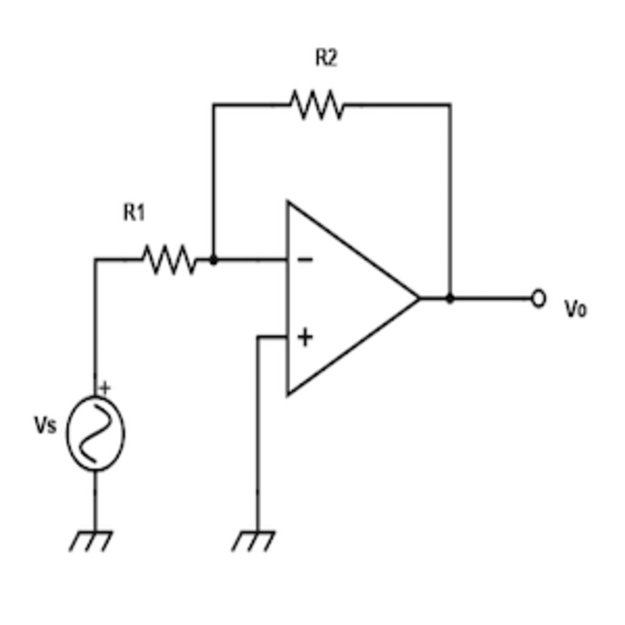
\includegraphics[width=.5\linewidth]{img/invertente.pdf}
\caption{Configurazione invertente}
\label{fig:invertente}
\end{subfigure}
\begin{subfigure}{.5\textwidth}
\centering
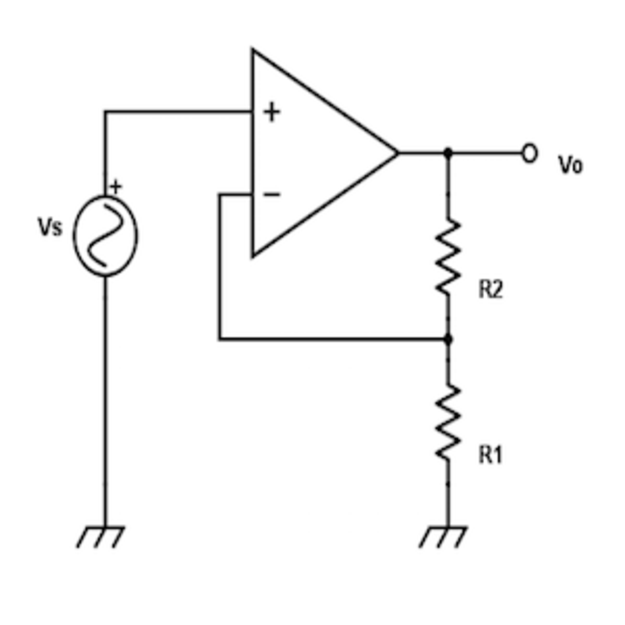
\includegraphics[width=.5\linewidth]{img/noninvertente.pdf}
\caption{Configurazione non invertente}
\label{fig:noninvertente}
\end{subfigure}
\begin{subfigure}{.5\textwidth}
\centering
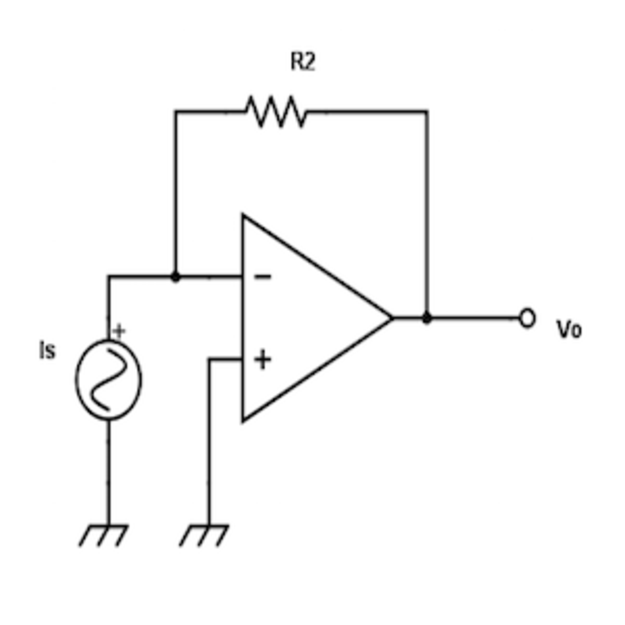
\includegraphics[width=.5\linewidth]{img/transresistenza.pdf}
\caption{Configurazione in transresistenza}
\label{transresistenza}
\end{subfigure}
\begin{subfigure}{.5\textwidth}
\centering
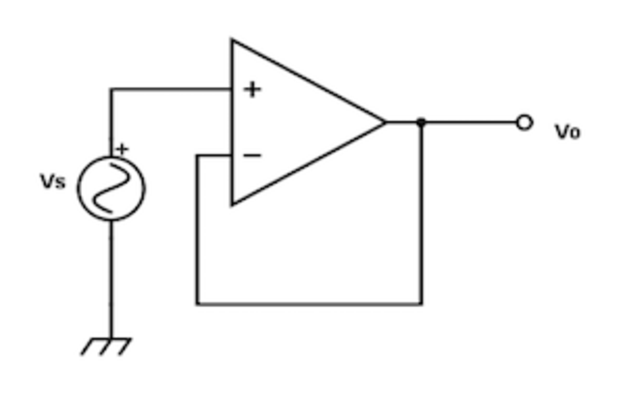
\includegraphics[width=.5\linewidth]{img/bufferunitario.pdf}
\caption{Buffer a guadagno unitario}
\label{fig:bufferunitario}
\end{subfigure}
\begin{subfigure}{.5\textwidth}
\centering
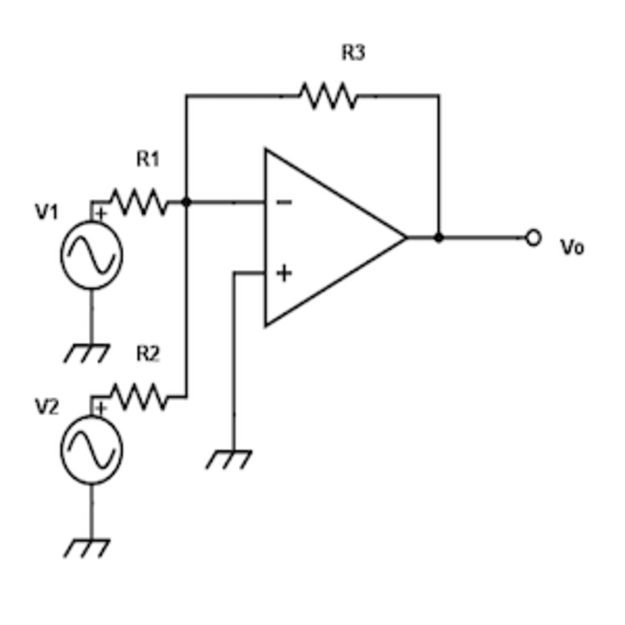
\includegraphics[width=.5\linewidth]{img/sommatore.pdf}
\caption{Configurazione sommatore}
\label{fig:sommatore}
\end{subfigure}
\begin{subfigure}{.5\textwidth}
\centering
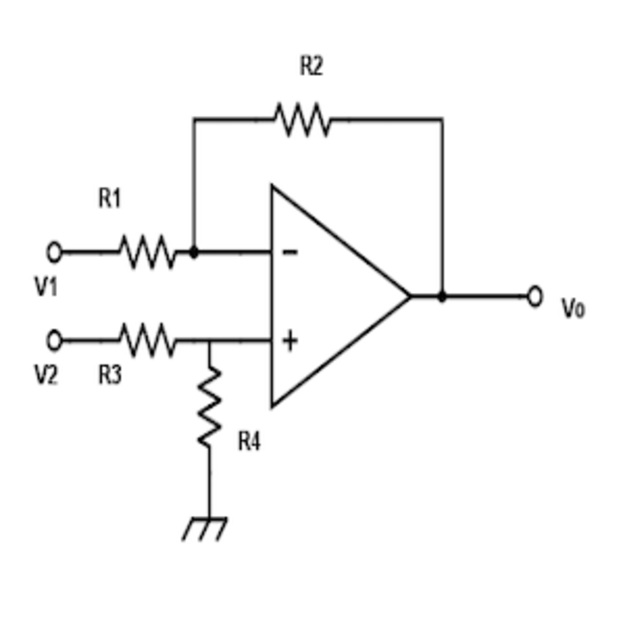
\includegraphics[width=.5\linewidth]{img/sottrattore.pdf}
\caption{Configurazione sottrattore}
\label{fig:sottrattore}
\end{subfigure}
\caption{Configurazioni di amplificatori}
\end{figure}

\section{Filtri}
Alcune considerazioni sui filtri che si possono realizzare con un OpAmp, un condensatore e qualche resistore. 
Ecco le impedenze dei tre principali componenti. La variabile complessa $s$ vale $s = \omega j$.

\begin{table}[H]
\begin{center}
\begin{tabular}{|l|l|}
\hline resistore & $Z_R = R$\\
\hline condensatore & $Z_C = 1/sC$\\
\hline induttore & $Z_L = sL$\\
\hline
\end{tabular}
\end{center}
\end{table}

Le funzioni di trasferimento delle configurazioni non invertente e invertente sono rispettivamente:
\begin{center}
$W(s) = {V_o(s) \over V_s(s)} = 1 + {Z_2 \over Z_1}$ \qquad $W(s) = -{Z_2 \over Z_1}$
\end{center}

\begin{table}[H]
\begin{center}
\begin{tabular}{|l|l|}
\hline
\hline & funzione di trasferimento\\
\hline
\hline \rule[-4mm]{0mm}{1cm} integratore & $-{1 \over sCR_1}$\\
\hline derivatore & $-sCR_2$\\
\hline
\end{tabular}
\end{center}
\end{table}

\textbf{Integratore.} Relazioni da ricordare:
\begin{center}
$i_c = C\frac{dv_c}{ dt}$ \qquad $v_o(t) = -{1 \over RC}\int_0^tv_s(\tau)d\tau + v_o(0)$
\end{center}

\textbf{Derivatore.} Relazioni da ricordare:
\begin{center}
$i_s = C\frac{dv_s}{ dt}$ \qquad $v_o = -RC\frac{dv_s}{dt}$
\end{center}

\begin{figure}[H]
\begin{subfigure}{.5\textwidth}
\centering
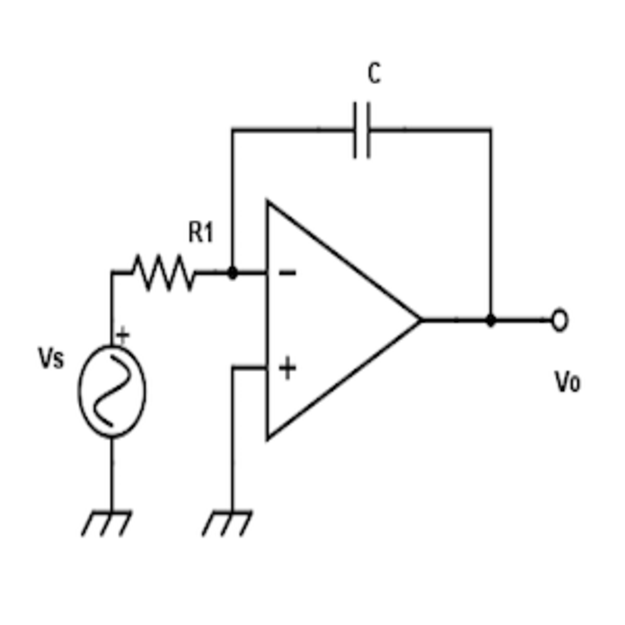
\includegraphics[width=.5\linewidth]{img/integratore.pdf}
\caption{Filtro integratore}
\label{fig:integratore}
\end{subfigure}
\begin{subfigure}{.5\textwidth}
\centering
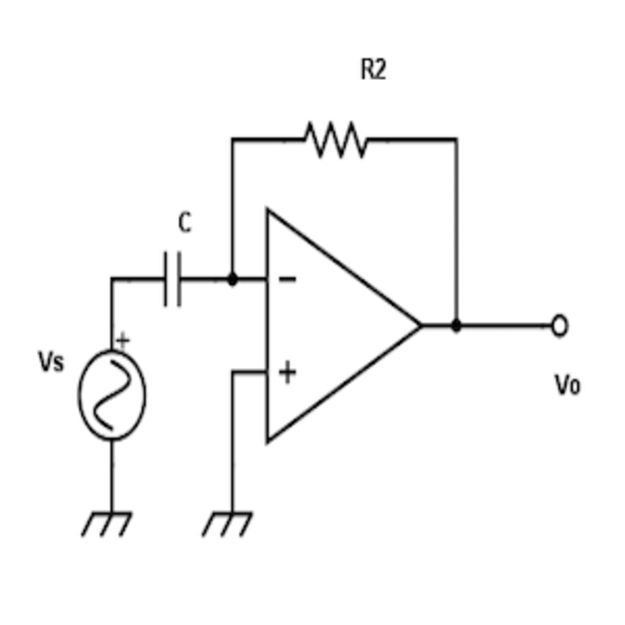
\includegraphics[width=.5\linewidth]{img/derivatore.pdf}
\caption{Filtro derivatore}
\label{fig:derivatore}
\end{subfigure}
\end{figure}

\begin{table}[H]
\begin{center}
\begin{tabular}{|l|l|}
\hline
\hline & funzione di trasferimento\\
\hline
\hline \rule[-4mm]{0mm}{1cm} passa basso & $-{R_2 \over R_1}{1 \over 1 + sCR_2}$\\
\hline \rule[-4mm]{0mm}{1cm} passa alto & $-{R_2 \over R_1}{s \over s + {1 \over CR_1}}$\\
\hline \rule[-4mm]{0mm}{1cm} passa banda & $-{C_1R_2 \over (1 + sC_1R_1)(1 + sC_2R_2)}$\\
\hline
\end{tabular}
\end{center}
\end{table}

\textbf{Passa Basso.} L'impedenza $Z_2$ è realizzata con il parallelo di condensatore e resistenza. 
Caratterizzato da guadagno a bassa frequenza $A_0 = -R_2 / R_1$ e frequenza di taglio $\omega_H = {1 
\over CR_2}$. Amplifica le frequenze al di sotto di $\omega_H$ per le quali si comporta come un amplificatore 
invertente di guadagno $A_0$.
\bigskip

\textbf{Passa Alto.} L'impedenza $Z_1$ è realizzata con la serie di un condensatore e resistenza. 
Caratterizzato da guadagno ad alta frequenza $A_0 = -R_2/R_1$ e frequenza di taglio $\omega_L = {1 \over 
CR_1}$. Amplifica le frequenze al di sopra di $\omega_L$.
\bigskip

\textbf{Passa Banda.} La fusione del passa basso e del passa alto.
\bigskip

\begin{figure}[H]
\begin{subfigure}{.5\textwidth}
\centering
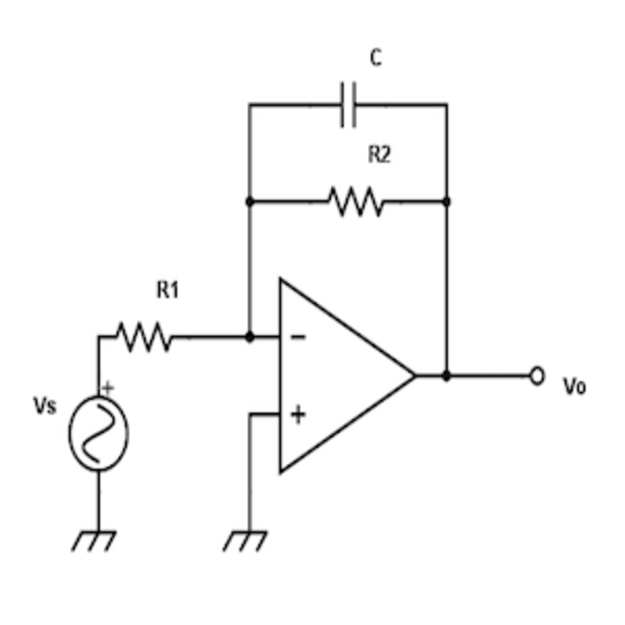
\includegraphics[width=.5\linewidth]{img/passabasso.pdf}
\caption{Filtro passa basso}
\label{fig:passabasso}
\end{subfigure}
\begin{subfigure}{.5\textwidth}
\centering
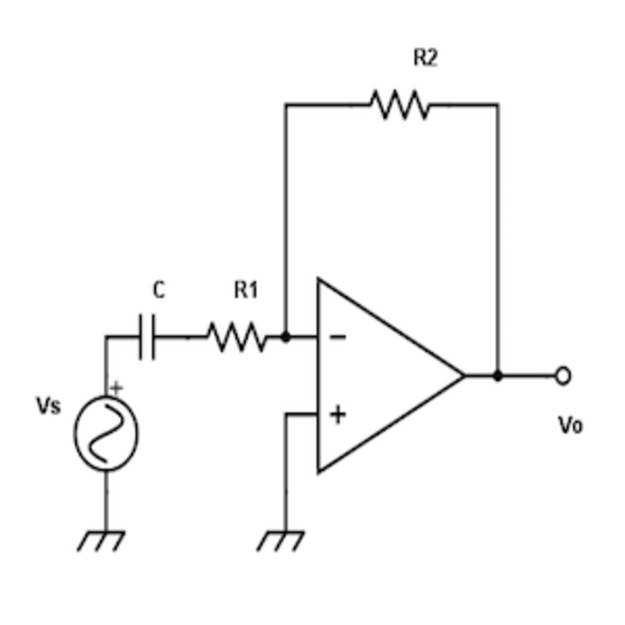
\includegraphics[width=.5\linewidth]{img/passaalto.pdf}
\caption{Filtro passa alto}
\label{fig:passaalto}
\end{subfigure}
\begin{subfigure}{.5\textwidth}
\centering
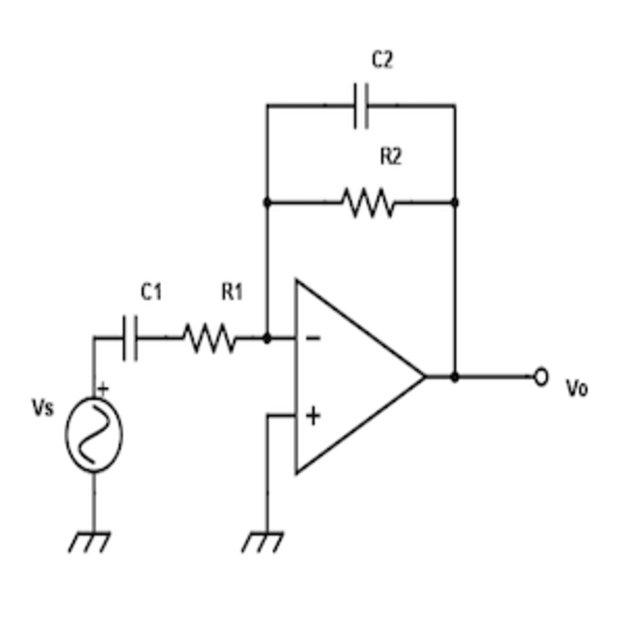
\includegraphics[width=.5\linewidth]{img/passabanda.pdf}
\caption{Filtro passa banda}
\label{fig:passabanda}
\end{subfigure}
\caption{Principali tipi di filtro}
\end{figure}

\section{Circuiti a retroazione positiva}

\textbf{Comparatore.}
\textbf{Trigger di Schmitt.}

\begin{figure}[H]
\begin{subfigure}{.5\textwidth}
\centering
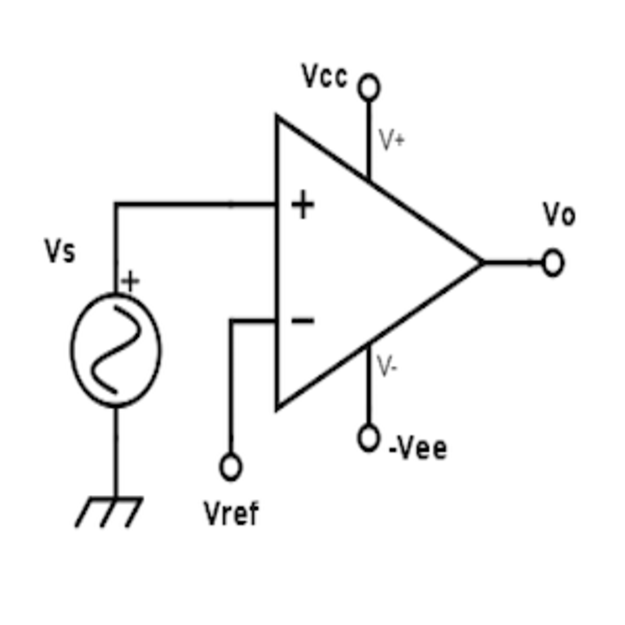
\includegraphics[width=.5\linewidth]{img/comparatore.pdf}
\caption{Circuito comparatore}
\label{fig:comparatore}
\end{subfigure}
\begin{subfigure}{.5\textwidth}
\centering
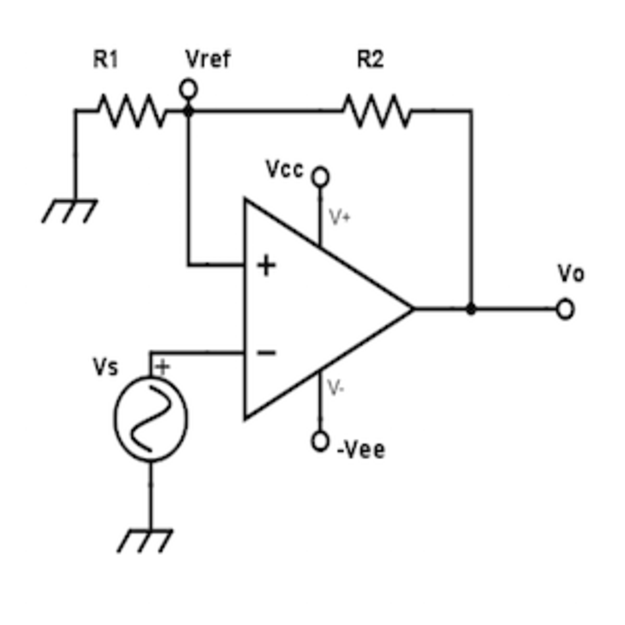
\includegraphics[width=.5\linewidth]{img/triggerschmitt.pdf}
\caption{Circuito trigger di Schmitt}
\label{fig:triggerschmitt}
\end{subfigure}
\end{figure}

\section{Semiconduttori}
\begin{center}
\textit{"La struttura atomica del silicio non gli consente di condurre elettricità, ma lui si droga e 
conduce ugualmente."} 
\end{center}
\hfill Antico detto ingegneristico\footnote{Taluni sostengono che il detto giunga 
dai dipartimenti di fisica. Questi "taluni" farebbero meglio a tacere, senza rancore.}\footnote{Le 
citazioni in questa forma vengono sempre inspiegabilmente attribuite ad A. Einstein.}.
\bigskip

\textbf{Materiali.} In base al parametro della \textit{resistività}, indicato con
$\rho$ e misurato in $\Omega \cdot cm$, si possono distinguere tre tipi di materiale: conduttori, 
semiconduttori e isolanti.
Si possono avere semiconduttori elementari (formati da atomi di un solo elemento) oppure semiconduttori 
composti. I più importanti semiconduttori elementari sono:
\textit{Boro} (B), \textit{Silicio} (Si), \textit{Fosforo} (P), \textit{Gallio} (Ga), \textit{Germanio} 
(Ge), \textit{Arsenico} (As), \textit{Indio} (In).\\Il Boro, appartenendo al III gruppo della tavola 
periodica, possiede \textit{3 elettroni di valenza nell'orbitale più esterno}, Silicio e Germanio ne 
hanno 4 mentre Fosforo e Arsenico 5.

\begin{table}[H]
\begin{center}
\begin{tabular}{|l|l|l|}
\hline
\hline Materiale & Resistività & Energy Gap\\
\hline 
\hline Isolanti & $\rho > 10^5$ & $E_G > 5\,eV$\\
\hline Semiconduttori & $ 10^{-3} < \rho < 10^5 $ & $ 0,5\,eV < E_G < 4\,eV$\\
\hline Conduttori & $ \rho < 10^{-3}$ & $E_G << kT$\\
\hline
\end{tabular}
\end{center}
\end{table} 

Nella forma cristallina, ogni atomo di Silicio forma 4 \textit{legami coovalenti} con altrettanti atomi e 
per temperature prossime allo 0 assoluto gli elettroni del livello più esterno se ne stanno al loro posto. 
Con l'aumentare della temperatura alcuni legami possono rompersi liberando elettroni. La densità di 
elettroni liberi è detta
\textit{concentrazione intrinseca}, indicata con $n_i$ e misurata in $cm^{-3}$, segue la relazione
\begin{center}
$n_i^2 = B T^3 \exp{-E_G \over k T}$
\end{center}
dove abbiamo:
\begin{itemize}
\item $E_G$ : \textit{energy gap}, ampiezza della banda proibita del semiconduttore ($1,12\,eV$ per il 
Silicio)
\item $k$ : costante di Boltzmann $8,62 \cdot 10^{-5} eV/K$ o  $1,38 \cdot 10^{-23} J/K$
\item $T$ : temperatura assoluta [K]
\item $B$ : parametro caratteristico del materiale ($1,08 \cdot 10^{31} K^{-3}cm^{-6}$ per il Silicio)
\end{itemize}
L'\textit{ampiezza della banda proibita} $E_G$ rappresenta la quantità di energia necessaria a rompere un 
legame covalente liberando un elettrone. Per un semiconduttore intrinseco (senza impurità) si ha che la 
densità di elettroni di conduzione $n$ e la densità di lacune $p$ è uguale a $n_i$.
\bigskip

\textbf{Semiconduttori drogati.} Se nel reticolo cristallino del Silicio vengono inseriti atomi di Boro 
oppure Fosforo o Arsenico abbiamo un semiconduttore drogato. Con Fosforo e Arsenico (che hanno 5 elettroni 
nel livello più esterno) si parla di
\textit{donatori} perchè questi forniscono un elettrone
e abbiamo un drogaggio di tipo $n$. Mentre con il Boro (che ha 3 elettroni) si parla di \textit{accettore} 
perchè fornisce una lacuna (uno spazio dove può stare un elettrone) e abbiamo un drogaggio di tipo $p$.\\

A temperatura ambiente $T = 300K$ e con $N_D >> n_i$ atomi donatori abbiamo $n \cong N_D$, similmente con 
$N_A >> n_i$ atomi accettori nel reticolo cristallino abbiamo $p \cong N_A$ dove $n$ e $p$ sono 
rispettivamente il numero di elettroni liberi (di conduzione) e il numero di lacune.\\

Sia EHP : electron/hole pair, il tasso di generazione G di EHP è funzione della temperatura quindi
$G = f_1(T)$ e il tasso di ricombinazione R è dato da
$R = n\,p\,f_2(T)$. All'equilibrio termodinamico $R = G$, si ottiene quindi la \textit{legge di azione di 
massa} e a seguire l'equazione di neutralità della carica:
\begin{center}
(AM) : $n\,p = n_i^2$ \quad (NC) : $q(N_D - p + N_A - n) = 0$
\end{center}
dalle quali si possono ricavare le concentrazioni di elettroni liberi e lacune in presenza di entrambe le 
specie droganti:
\begin{center}
Sostituendo $p = {n_i^2 \over n}$ in (NC) si ha $n = {(N_D - N_A) \pm \sqrt{(N_D - N_A)^2 + 4n_i^2} \over 
2}$
\end{center} 

\textbf{Corrente di deriva.} In inglese \textit{drift} è la corrente delle cariche mosse da un campo 
elettrico. Il moto complessivo degli elettroni ha componenti date da agitazione 
termica e campo elettrico, la velicità termica media è nulla. La velictà oltre una certa soglia tende a 
saturare, per il silicio $v_{sat} \cong 10^7 cm/s$. Alcune formule importanti da Fisica II:
\begin{center}
$v = -{q\,E \over m}t$,\quad$\mu_n = {q\,t \over m}$ da cui si ricava $I = -N_D\,\mu_n\,E\,q\,A = -J_n\,A$ 
\end{center}
Dove abbiamo:
\begin{itemize}
\item $v$ : velocità \textit{di deriva} dei portatori di carica (elettroni)
\item $\mu$ : mobilità dei portatori di carica (nel silicio
$\mu_n = 1350\,cm^2/Vs$ e $\mu_p = 500\,cm^2/Vs$) 
\item $I$ : corrente attraverso sezione A
\end{itemize}
Si ottiene quindi la densità di corrente di deriva totale e conducibilità del materiale:
\begin{center}
$j_T^{drift} = j_n + j_p = q(n\mu_n + p\mu_p)\,E$ \quad $\sigma = q(n\mu_n + p\mu_p)$ con $\sigma = 1/\rho$
\end{center}

\textbf{Corrente di diffusione.} Il drogaggio di solito non è costante (distribuzione non uniforme) e i 
portatori di carica liberi 
tendono a diffondere da zone a maggiore concentrazione verso altre dove questa è più bassa.
Gli elettroni diffondono infatti dove la carica è maggiore, per le lacune vale il contrario. La corrente 
di diffusione è data da:
\begin{center}
$j_n^{diff} = +q\,D_n{\partial n \over \partial x}$ \qquad $j_n^{diff}=-q\,D_p{\partial p\over \partial x}$
\end{center}
dove $D_n$ è la diffusività degli elettroni.
Diffusività e mobilità sono legate dalla
\textit{relazione di Einstein}
\begin{center}
${D_n \over \mu_n} = {k\,T \over q} = {D_p \over \mu_p}$ con $V_T = {k\,T \over q}$
\end{center}
dove $V_T$ è la tensione termica.
\bigskip

\textbf{Corrente totale.} La corrente totale (per lacune e elettroni) è data dalla somma della componente 
per diffusione e dalla componente di deriva (per le lacune cambia solo il segno $-$):
\begin{center}
$J_n(x) = q(n(x)\,E(x) + D_n{\partial n(x) \over \partial x})$
\end{center}

\textbf{Conclusioni.} Consideriamo la variazione nel tempo della concentrazione di elettroni (e similmente 
anche per le lacune, salvo segni) in un volume di area infinitesimale $A\,dx$ data dall'equazione
\begin{center}
${dn \over dt}A\,dx = -{1\over q}(J_n(x) - J_n(x + dx))A + (G-R)A\,dx$ che porta a
${dn \over dt} = {1\over q}{dJ_n\over dx} + (G-R)$
\end{center}
dalla quale, sostituendo $J_n$ si ottiene l'\textit{equazione di continuità}
\begin{center}
${dn \over dt} = \mu_nn{dE\over dx} + \mu_nE{dn\over dx} + D_n{d^2n\over dx^2} + (G-R)$
\end{center}

(vedere esempi di risoluzione equazione)


\section{Giunzione PN}

Cosa accade se si pongono due semiconduttori drogati \textit{p} e \textit{n} l'uno accanto all'altro? Per
rispondere a questa domanda potrebbe tornare utile pensare a cosa accadrebbe se ci fossero due feste, 
una del dipartimento di ingegneria e l'altra del dipartimento di psicologia, in due locali adiacenti. Bene,
all'ora x si aprono gli accessi che mettono in comunicazione i due locali e \textit{ovviamente} gli elettroni,
cioè i ragazzi \textit{liberi}, diffondono da un locale a maggior concentrazione maschile verso il locale
con il maggior numero di lacune da colmare (associazione $ragazze \to lacune$ è del tutto casuale, non vi è
alcun riferimento anatomico in tutto ciò). Allo stesso modo possiamo pensare che anche le ragazze preferiscano
fluire dalla loro noiosa festa dipartimentale verso la festa di ingegneria (e così avviene, anche se solo 
virtualmente).\\
 
Cercando di rispondere alla domanda iniziale, ponendo un semiconduttore \textit{p} accanto ad uno drogato 
\textit{n}, si genera una 
corrente di diffusione: gli elettroni in \textit{n} finiscono in \textit{p} e le lacune in \textit{p} 
finiscono in \textit{n}. Questo genera un campo elettrico \textit{E}, nei pressi della giunzione, che si 
oppone alla corrente di diffusione. Si raggiunge un equilibrio dinamico: $J^{drift} = J^{diff}$.
Il risultato è una regione di carica spaziale (RCS) compresa tra due regioni quasi neutre (RQN). Tuttavia 
nella RCS si hanno due diverse densità di carica
\begin{center}
$\rho(x) = -qN_A$ per $-x_p<x<0$ \quad e \quad $\rho(x) = qN_D$ per $0<x<x_n$.
\end{center}
Con l'equazione di Poisson si ottiene
\begin{center}
(Poisson) ${d\,E \over d\,x} = {\rho \over \epsilon_s}$ \quad e \quad $E = -{d\,V \over d\,x}$
\end{center}
All'equilibrio la corrente totale (paragrafo precedente) è nulla, quindi vale:
\begin{center}
$q\,\mu_n(x)\,n\,E(x) = -q\,D_n\,{dn \over dx}$ \quad (con eq. Einstein) \quad $dV = V_T{1 \over n}dn$
\end{center}
conoscendo le concentrazioni di elettroni e lacune nelle RQN, date da
regione \textit{p}: $n_p = {n_i^2 \over N_A}$, regione \textit{n}: $n_n = N_D$, si ottiene
\begin{center}
$V_2 - V_1 = V_T \ln({n_2 \over n_1})$
\end{center}
La lunghezza della regione di svuotamento si ottiene dall'equazione
\begin{center}
$W_{dep} = x_p + x_n = \sqrt{{2\,\epsilon_s \over q}({1\over N_A} + {1\over N_D})V_0}$ \quad ${x_n \over 
x_p} = {N_A \over N_D}$
\end{center}

\textbf{Giunzione PN polarizzata.} Si collega un generatore di tensione $V_A$ collegando polo $+$ alla 
regione $p$ e polo $-$ alla regione $n$. Se $V_A < 0$ si è in regime di polarizzazione inversa e la 
tensione  di sbarramento aumenta. Se $V_A > 0$ si è in polarizzazione diretta e la tensione di 
sbarramento diminuisce.


\section{Diodo}

Il diodo é un componente elettronico che funziona come una valvola: se la tensione applicata ai suoi capi 
è positiva, il diodo fa passare corrente, altrimenti non conduce. Modificando la tensione ai capi di un
diodo si modifica infatti il \textit{potenziale di giunzione} indicato con $\Phi_j$, la barriera che
limita lo spostamento delle cariche.\\
Per tensioni inferiori a $-0,1 V$ la corrente non è zero ma tende ad un valore constante, la corrente di
saturazione $-I_S$. L'equazione che permette di modellizzare questo comportamento è
\begin{center}
$i_D = I_S (\exp({v_D \over V_T} - 1))$
\end{center}
dove:
\begin{itemize}
\item $I_S$ : corrente di saturazione inversa del diodo $[A]$
\item $v_D$ : tensione ai capi del diodo $[V]$
\end{itemize}
\bigskip

\textbf{Polarizzazione del diodo.} Un diodo può trovarsi in sole due regioni di funzionamento, la \textit{
polarizzazione inversa} per $v_D < 0$ e la \textit{polarizzazione diretta} per $v_D > 0$.
\begin{itemize}
\item in inversa solo una piccola quantità di corrente (approssimabile a $I_S$) fluisce attraverso il diodo
	che viene considerato spento.
\item in diretta la corrente attraverso il diodo cresce esponenzialmente rispetto alla tensione e si può
	assumere $i_D \approx I_S \exp{v_D / V_T}$.
\end{itemize}

\begin{figure}[H]
\centering
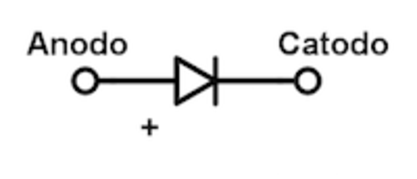
\includegraphics[width=.3\linewidth]{img/diodo.pdf}
\caption{Simbolo circuitale del diodo}
\label{fig:diodo}
\end{figure}

\textbf{Modelli circuitali.} Ci sono tre modelli per semplificare il funzionamento di un diodo nei circuiti:
\begin{itemize}
\item \textit{diodo ideale}, quando il diodo è in conduzione lo si sostituisce con un cortocircuito;
\item \textit{caduta di tensione costante}, quando il diodo è in conduzione lo si sostituisce con un 
	generatore di tensione ideale $V_{on}$;
\item \textit{caduta di tensione con resistore}, quando il diodo è in conduzione lo si sostituisce con la
	serie generatore di tensione ideale e resistore.
\end{itemize}
Il diodo è in conduzione quando $V_D > 0$, in caso contrario in tutti i modelli lo si sostitisce con un 
cirtuito aperto.
\bigskip

\textbf{Circuito raddrizzatore a semionda.} Questo semplice circuito è molto diffuso e viene utilizzato negli
alimentatori che convertono una tensione ac (sinusoidale) in una dc. Il diodo "raddrizza" la sinusoide e un
filtro capacitivo stabilizza poi la tensione.\\
Il raddrizzatore a semioda è una serie di generatore di tensione $v_S = V_P \sin (\omega t)$, diodo $D_1$ e
resistenza $R$. Può capitare che la tensione di polarizzazione $V_{on}$ del diodo sia significativa, la 
tensione di uscita diventa quindi $v_O = V_P \sin (\omega t) - V_{on}$. La tensione in uscita non può essere
utilizzata da apparecchi elettronici, serve un condensatore di filtraggio.
\bigskip

\textbf{Raddrizzatore con filtro capacitivo.} Il circuito \textit{rilevatore di picco} è come il precedente,
ma al posto del resistore c'è un condensatore $C$. Una volta che la tensione raggiunde il picco $V_P$ 
resta costante a questo valore poichè non c'è nulla che scarichi il condensatore (il diodo è sempre in 
interdizione perché la tensione su $C$ è più elevata di $v_S$).
\bigskip

\textbf{Raddrizzatore con carico RC.} In questo caso la tensione d'uscita non è costante ma caratterizzata da
una tensione di ondulazione, \textit{ripple voltage}, $V_r$ e il diodo conduce per un intervallo di tempo
$\Delta T$. Con l'equazione della scarica del condensatore si ha:
\begin{center}
$V_r = (V_P - V_{on}) v_O(t') = (V_P - V_{on}) \left(1-\exp(-{T - \Delta T \over RC})\right)$.
\end{center}
Per quanto riguarda l'intervallo di conduzione del diodo $\Delta T$, questo si ricava con l'intersezione
delle curve della tensione in entrata (sinusoide, ricordando $\sin(t' + T - \Delta T) = \cos(T - \Delta T)$) 
e della scarica del condensatore (esponenziale) quindi:
\begin{center}
$(V_P-V_{on})\exp(-{T-\Delta T \over RC})=V_P\cos(\omega(T-\Delta T)) - V_{on}$.
\end{center}
Con le semplificazioni di Taylor e assumendo $\Delta T \ll T$ la tensione di ondulazione, l'intervallo di 
e l'angolo di conduzione valgono:
\begin{center}
$V_r \cong {V_P - V_{on} \over R}{T \over C}$ \quad $\Delta T \cong {1 \over \omega}\sqrt{{2V_r \over V_P}}$
\quad $\theta_c = \omega \Delta T = \sqrt{{2V_r \over V_P}}$.
\end{center}
\bigskip

\textbf{Corrente di picco.} Il diodo è attraversato da corrente solamente durante il breve periodo $\Delta T$
Il valore massimo che assume (tralasciando il valore iniziale, detto \textit{corrente di spunto}) viene
detto \textit{corrente di picco}. Questa ha forma di un triangolo di altezza $I_P$ e base $\Delta T$ la cui
area corrisponde alla carica $Q = I_{dc} T$ (da $dq = i\,dt$), quindi
\begin{center}
$I_P = I_{dc} {2T \over \Delta T}$ \quad dove \quad $I_{dc} = {V_P - V_{on} \over R}$.
\end{center}
\bigskip

\begin{figure}[H]
\begin{subfigure}{.5\textwidth}
\centering
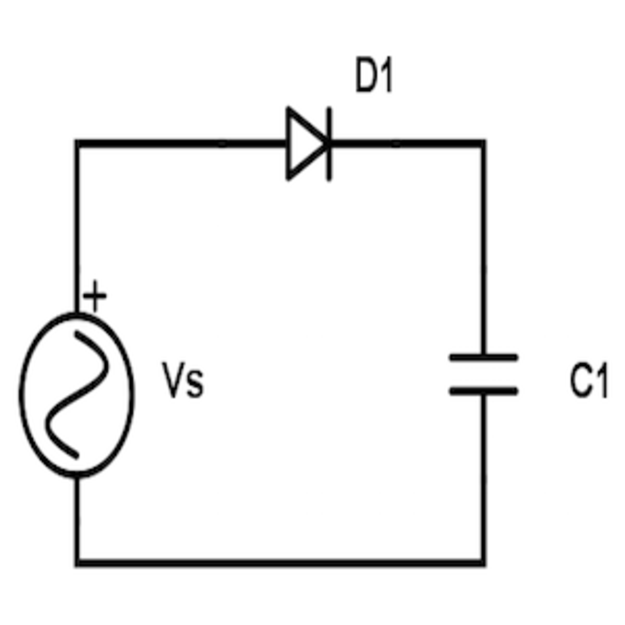
\includegraphics[width=.5\linewidth]{img/raddcap.pdf}
\caption{Circuito raddrizzatore con filtraggio}
\label{fig:integratore}
\end{subfigure}
\begin{subfigure}{.5\textwidth}
\centering
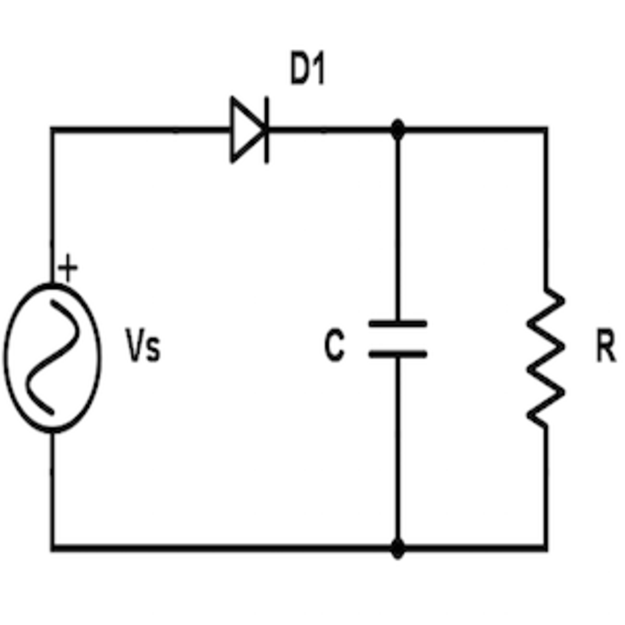
\includegraphics[width=.5\linewidth]{img/raddRC.pdf}
\caption{Circuito raddrizzatore con carico RC}
\label{fig:derivatore}
\end{subfigure}
\begin{subfigure}{.5\textwidth}
\centering
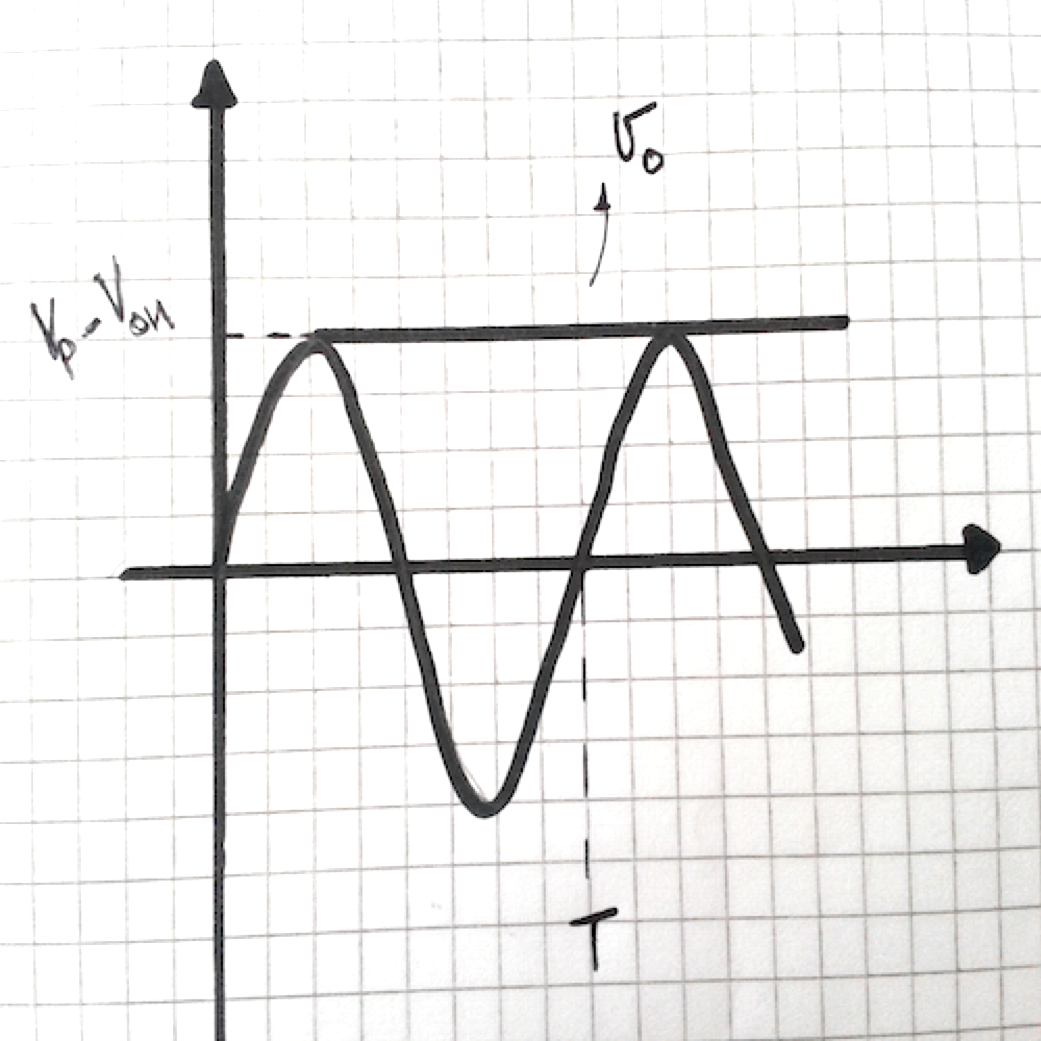
\includegraphics[width=.5\linewidth]{img/uscitaraddcap.pdf}
\caption{Tensione di uscita raddrizzatore con filtraggio}
\label{fig:integratore}
\end{subfigure}
\begin{subfigure}{.5\textwidth}
\centering
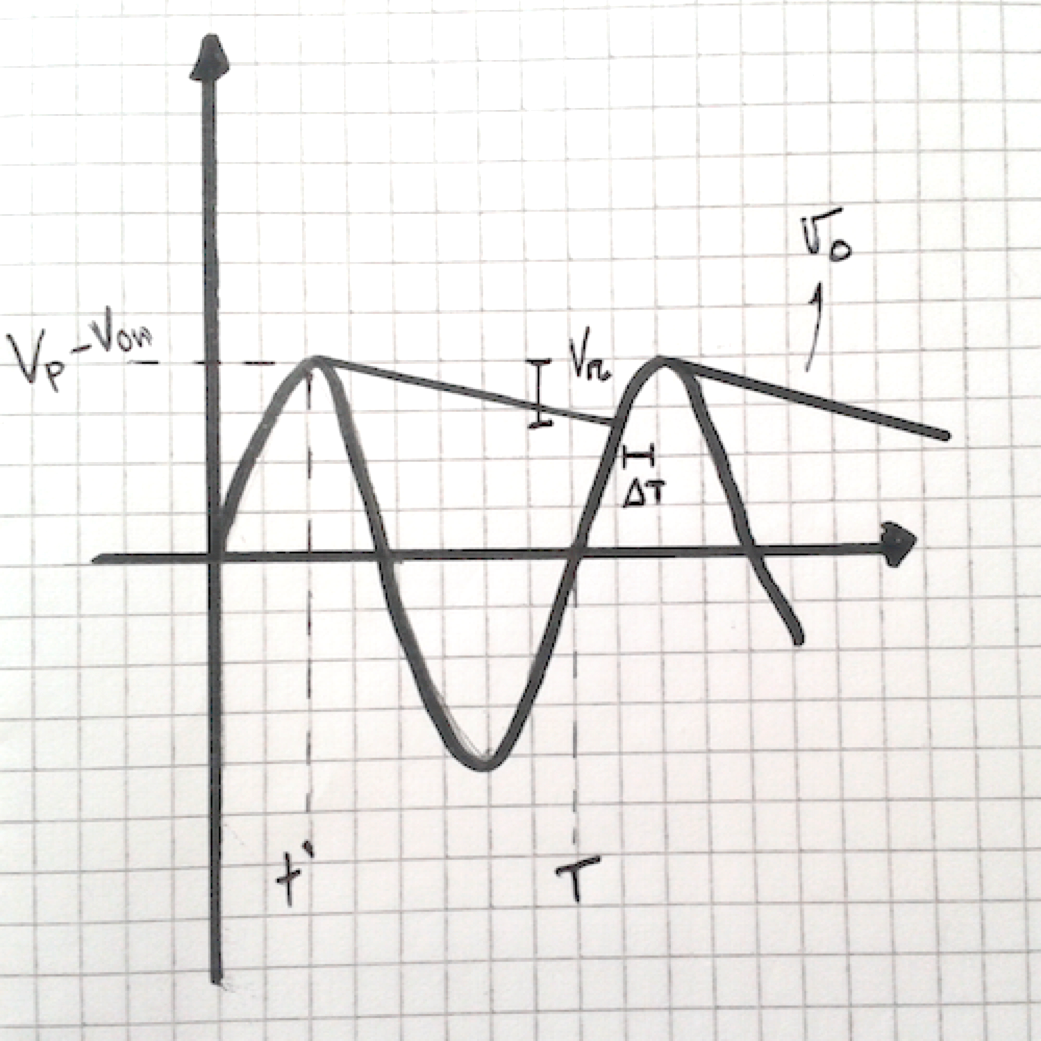
\includegraphics[width=.5\linewidth]{img/uscitaraddRC.pdf}
\caption{Tensione di uscita raddrizzatore con carico RC}
\label{fig:integratore}
\end{subfigure}
\end{figure}

\textbf{Raddrizzatore a doppia semionda.} Utilizzando un trasformatore a presa centrale che genera due 
sinusoidi sfasate di $180^{\circ}$ e due diodi, si può realizzare un circuito che dimezza il tempo di 
scarica del condensatore. Infatti per $v_S > 0$, $D_1$ è in conduzione mentre per $v_S < 0$ lo è $D_2$. 
Si ha quindi che $V_r = {V_P - V_{on} \over RC}{T \over 2}$.
\bigskip

\textbf{Raddrizzatore a ponte a doppia semionda.} Con l'aggiunta di due diodi allo schema precedente si 
può ottenere un \textit{ponte di diodi} che consente di utilizzare un trasformatore semplice per ottenere
lo stesso effetto. In questo caso per $v_S>0$, $D_1$ e $D_3$ conducono, per $v_S<0$ conducono $D_2$ e $D_4$.
\bigskip

\begin{figure}[H]
\begin{subfigure}{.5\textwidth}
\centering
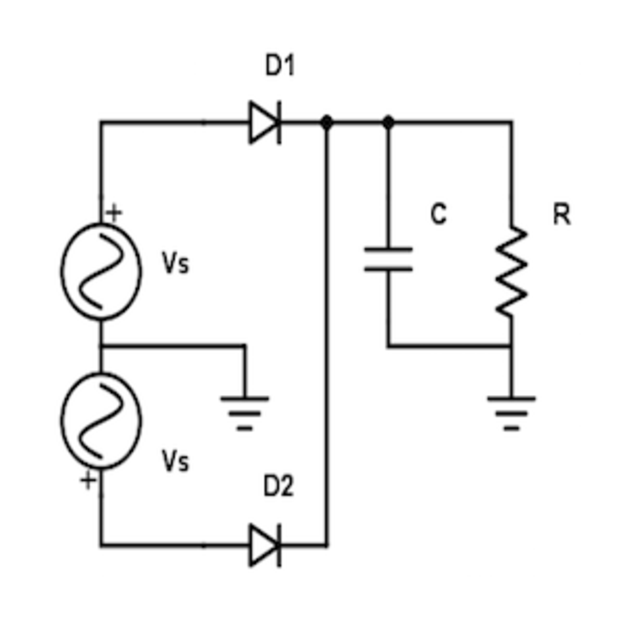
\includegraphics[width=.5\linewidth]{img/radd.pdf}
\caption{Circuito raddrizzatore a doppia semionda}
\label{fig:integratore}
\end{subfigure}
\begin{subfigure}{.5\textwidth}
\centering
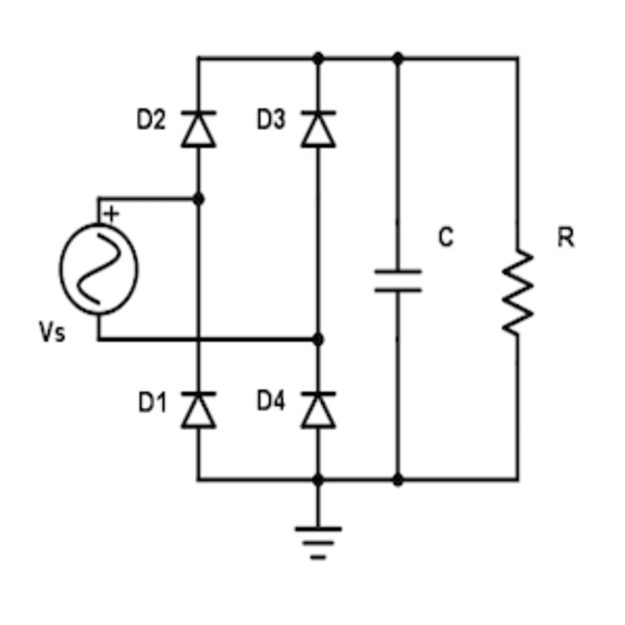
\includegraphics[width=.5\linewidth]{img/raddponte.pdf}
\caption{Circuito raddrizzatore a ponte a doppia semioda}
\label{fig:derivatore}
\end{subfigure}
\end{figure}


\section{Transistor a effetto di campo}

La tecnologia FET (Field Effect Transistor) più diffusa è la MOS (Metal-Oxide Transistor), utilizzata 
soprattutto per i circuiti VLSI (Very Large Scale Integration). Tuttavia i tradizionali NMOS e PMOS, dissipano
molta poteza e per questo si è passati ad una tecnologia CMOS (ovvero una strutture composta da un NMOS e un
PMOS), più costosa e complessa da realizzare ma che porta ad una riduzione della potenza dissipata.
\bigskip

\textbf{Condensatore MOS.} Il condensatore MOS è il cuore della tecnologia: è composto da uno strato isolante,
tipicamente diossido di silicio $SiO_2$, frapposto ad un elettrodo metallico (di solito alluminio) chiamato
\textit{Gate}, ed un supporto drogato $p$ o $n$, chiamato \textit{Body}.\\
A seconda di quanto vale la tensione applicata al Gate $V_G$, in relazione ad una tensione di soglia detta
$V_{TN}$ si possono distinguere i seguenti casi (assumendo un substrato $p$):
\begin{itemize}
\item \textit{regione di accumulazione}, quando $V_G \ll V_{TN}$ e $V_G$ negativa rispetto al substrato, 
	allora si forma uno strato di accumulazione di lacune al di sotto dell'isolante;
\item \textit{regione di svuotamento}, per $V_G < V_{TN}$, con l'aumentare della tensione $V_G$ si forma
	una regione di svuotamento;
\item \textit{regione di inversione}, per $V_G > V_{TN}$, allora, superata la tensione di soglia, si forma 
	uno strato di elettroni (detto di inversione), al di sotto dell'isolante.
\end{itemize} 
\bigskip

\textbf{NMOS.} Un MOSFET a canale $n$ si realizza aggiungendo ai lati di un condensatore MOS due regioni con 
forte drogaggio $n$, quindi $n^+$, chiamate \textit{Drain} e \textit{Source}. Due parametri importanti del 
transistor sono la lunghezza del canale $L$ e la larghezza del Body $W$.\\
Allo stesso modo di come funziona il condensatore MOS, così funziona il transistor con l'aggiunta che quando
ci si trova in inversione e si applica una tensione $v_{DS}$ positiva si crea una correte di elettroni dal
Source al Drain. Questo dispositivo viene detto transistor NMOS ad \textit{arricchimento} 
(\textit{Enhancement}).    
\bigskip

\textbf{Regione di triodo del NMOS.} La regione di triodo, che viene spesso chiamata regione lineare, è la
regione di funzionamento in cui $V_{GS} > V_{TN}$ e $V_{DS} < V_{GS} - V_{TN}$, ovvero si è formato il canale
$n$ perché si è superata la tensione di soglia e questo non viene strozzato da un'eccessiva corrente di Drain.
In queste condizioni si ha (dalla formula del condensatore)
\begin{center}
$i_S = i_D$ \quad e \quad $dq(x) = -C_{OX}''Wdx (V_{GS} - V(x) - V_{TN})$
\end{center}
dove
\begin{itemize}
\item $C_{OX} = {\epsilon_{OX} \over T_{OX}}$ è la capacità relativa all'ossido per unità di area $[F]/[cm]^2$;
\item $\epsilon_{OX}$ è la permettività dell'ossido in $[F]/[cm]$;
\item $T_{OX}$ è lo spessore dell'ossido;
\item $W$ è la larghezza del canle.
\end{itemize}
Sapendo che il campo elettrico lungo il canale vale $E = - dV(x)/dx$ e che questo induce una velocità
di deriva pari a $dx/dt = - \mu_n E(x)$ derivando tutto rispetto al tempo e integrando sulla lunghezza $L$ 
si ottiene (ponendo $I = -I_D$)
\begin{center}
$I = -\mu_n C_{OX} W (V_{GS} - V(x) - V_{TN} {dV(x) \over dx})$ \quad $\int_0^L I_Ddx = 
\int_0^{V_{DS}} \mu_n C_{OX} W (V_{GS} - V(x) - V_{TN})dV(x)$.
\end{center}
Si ottengono quindi rispettivamente, la relazione valida nella zona di triodo e quella valida in saturazione
(ponendo $V_{DS} = V_{GS} - V_{TN}$)
\begin{center}
$I_D = \mu_n C_{OX} {W \over L} \left((V_{GS} - V_{TN}) V_{DS} - {V_{DS}^2 \over 2}\right)$.
\end{center}
\bigskip


\section{Transistor a giunzione bipolare}

\textbf{Struttura.} Il transistor a giunzione bipolare (BJT) è costituito da 3 parti: l'emettitore, la base
e il collettore. Ognuna di queste regioni è drogata \textit{n} o \textit{p} e si possono avere 2 
configurazioni: \textit{npn} e \textit{pnp}.
\bigskip

\textbf{Transistor NPN.} Dall'analisi delle caratteristiche in funzionamento diretto e inverso si ricavano
le seguenti equazioni, che forniscono un buon modello matematico del funzionamento di un transistor
(\textit{modello di trasporto}, versione semplificata del modello di Gummel-Poon).
\begin{center}
$i_C=I_s[\exp{{v_{BE} \over V_T}}-\exp{{v_{BC} \over V_T}}]-{I_s \over \beta_R}[\exp{{v_{BC} \over V_T}}-1]$\\
$i_E=I_s[\exp{{v_{BE} \over V_T}}-\exp{{v_{BC} \over V_T}}]+{I_s \over \beta_F}[\exp{{v_{BE} \over V_T}}-1]$\\
$i_B={I_s \over \beta_F}[\exp{{v_{BE} \over V_T}-1}]+{I_s \over \beta_R}[\exp{{v_{BC} \over V_T}}-1]$
\end{center}
dove compaiono i parametri:
\begin{itemize}
\item $\beta_F$: guadagno di corrente diretto a emettitore comune
\item $\beta_R$: guadagno di corrente inverso a emettirore comune 
\end{itemize}
Per il BJT pnp le equazioni sono le stesse ma le tensioni $v_{BE}$ e $v_{BC}$ vanno prese in senso
opposto e diventano quindi $v_{EB}$ e $v_{CB}$.
\bigskip

\textbf{Regioni di funzionamento.} Ciascuna delle regioni pn del BJT può essere polarizzata in modo diretto 
o in modo inverso, questo comporta che un transistor può trovarsi in quattro regioni di funzionamento.
Il \textit{punto di lavoro} determina la regione di funzionamento del BJT ed è definito dal valore di due
delle quattro possibili tensioni o correnti ai terminali, come ad esempio $(I_C,V_{CE})$. Le regioni sono:
\begin{itemize}
\item \textit{Interdizione}: entrambe le giunzioni sono polarizzate inversamente, il BJT si comporta come 
	un circuito aperto.\\ 
	Per semplificare il modello si assimono $v_{BE},v_{BC} \le 0$, spariscono tutti i termini con 
	esponenziale e si ottengono
	\begin{center}
	$i_C = {I_S \over \beta_R}$ \quad $i_E = -{I_S \over \beta_F}$ \quad 
	$i_B = -I_S({1 \over \beta_F} + {1 \over \beta_R)}$
	\end{center}
\item \textit{Saturazione}: entrambe le giunzioni sono polarizzate direttamente, il BJT si comporta come 
	un corto circuito. Queste due prime regioni vengono utilizzate nei circuiti digitali TTL (transistor-
	transistor logic) per rappresentare gli stati della logica binaria.\\
	Per semplificare il modelllo si assume $v_{BC} \le 0$ per cui spariscono tutti i termini 
	esponenziali con BC e si ottengono
	\begin{center}
	$i_C = I_S \exp{{V_{BE}\over V_T}} + {I_S \over \beta_R}$ \quad 
	$i_E = {I_S \over \alpha_F} \exp{{v_{BE} \over V_T}} + {I_S \over \beta_F}$ \quad
	$i_B = {I_S \over \beta_F} \exp{{v_{BE} \over V_T}} -I_S({1\over \beta_F}+{1\over \beta_R})$
	\end{center}
	Semplificando ulteriormente si possono togliere tutti i termini non esponenziali e si hanno le 
	relazioni
	\begin{center}
	$i_C = \alpha_F i_E$ \quad $i_C = \beta_F i_B$ \quad $i_E = (\beta_F + 1)i_B$
	\end{center}
\item \textit{Attiva diretta}: la giunzione BE è polarizzata direttamente mentre BC è in inversa. In questa
	regione il BJT ha ottimi guadagni in tensione, corrente e potenza e viene quindi polarizzato in
	questo modo nei circuiti analogici per amplificare.
\item \textit{Attiva inversa}: la giunzione BE è in inversa mentre BC è in diretta. Regione raramente 
	utilizzata. 
\end{itemize}
\bigskip


\section{Modelli a piccolo segnale}

\textbf{Circuiti equivalenti.} Per poter analizzare più facilmente circuiti con molti elementi sia per 
tensioni constanti che alternate si apportano delle semplificazioni:
\begin{itemize}
\item \textit{circuito equivalente in dc}: condensatori $\to$ circuiti aperti, induttori $\to$ cortocircuiti;
\item \textit{circuito equivalente in ac}: condensatori $\to$ cortocircuiti, induttori $\to$ circuiti aperti 
	(si assume $\omega \to \infty$).
\end{itemize}
I passi da seguire per analizzare un circuito sono quindi:
\begin{enumerate}
\item ottenere il circuito equivalente in dc;
\item deteminare il punto di lavoro con il modello ampli per il transistor;
\item ottenere il circuito equivalente in ac;
\item sostituire transistor con modello a piccolo segnale;
\item analizzare caratteristiche ac dell'ampli;
\item combinare risultati in ac e dc per ottenere i valori complessivi della tensione.
\end{enumerate}
\bigskip

\textbf{Diodo.} I parametri di cui bisogna tenere conto per descrivere un diodo al piccolo segnale sono:
\begin{itemize}
\item $i_D = I_D + g_d v_d$;
\item $i_d = g_d v_d$;
\item $g_d = {I_D + I_S \over V_T} \cong {I_D \over V_T} \cong 40 I_D$ essendo $V_T$ la tensione termica.
\end{itemize}
$g_d$ è la conduttanza per piccoli segnali o conduttanza differenziale. Affiché queste equazioni valgano 
si deve avere la \textit{condizione di piccolo segnale}
\begin{center}
$\left|v_d\right| < 5 mV$ \quad e \quad $\left|i_d\right| < 0.2 I_D$.
\end{center}
\bigskip

\textbf{BJT.} I parametri per descrivere un BJT a piccolo segnale sono i seguenti:
\begin{itemize}
\item $g_m = {I_C \over V_T} \cong 40 I_C$;
\item $g_m v_{be} = \beta_0 i_b$, può tornare utile vederlo in entrambi i modi;
\item $r_{\pi} = {\beta_0 \over g_m}$;
\item $r_o = {V_A + V_{CE} \over I_C} \cong {V_A \over I_C}$ dove $V_A$ è la tensione di Early.
\end{itemize}
Spesso $r_0$ può essere trascurata (sostituendola con un circuito aperto) per i calcolo del guadagno in 
tensione, se risulta $A_v \ll \mu_f$. Le condizioni di piccolo segnale per il BJT sono
\begin{center}
$\left|v_{be}\right| < 5 mV$ \quad e \quad $\left|i_c\right| < 0.2 I_C$.
\end{center}
\bigskip

\textbf{MOSFET.} Per quanto riguarda la descrizione a piccolo segnale di un MOSFET abbiamo:
\begin{itemize}
\item $r_o = {{1 \over \left|\lambda \right|} + \left|V_{DS}\right| \over I_D} \cong {1 \over \left|\lambda
	\right| I_D}$;
\item $g_m = {2 I_D \over V_{GS} - V_{TN}} = \sqrt{2 K_n I_D (1 - \lambda V_{DS})} = {2 \over \left|V_{TN}
	\right|} \sqrt{I_{DSS} I_D (1 + \lambda V_{DS})}$ essendo $I_{DSS} = {K_n V_{TN}^2 \over 2}$.
\end{itemize}
Queste relazioni valgono per
\begin{center}
$v_{gs} \le 0.2 (V_{GS} - V_{TN})$ \quad e \quad $i_d \le 0.4 I_D$.
\end{center}
\bigskip

\begin{figure}[H]
\begin{subfigure}{.5\textwidth}
\centering
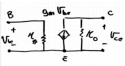
\includegraphics[width=.5\linewidth]{img/bjtpiccolo.pdf}
\caption{Circuito equivalente BJT a piccolo segnale}
\label{fig:integratore}
\end{subfigure}
\begin{subfigure}{.5\textwidth}
\centering
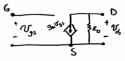
\includegraphics[width=.5\linewidth]{img/mospiccolo.pdf}
\caption{Circuito equivalente MOSFET a piccolo segnale}
\label{fig:derivatore}
\end{subfigure}
\end{figure}

\textbf{Amplificatore a emettitore comune.}
\bigskip

\section{Esercizi}

Esercizi di elettronica presi dal simulatore.


\subsection{Esercizio}

Difficoltà: ***\\

Il circuito di figura \ref{img:transdiodo1}, che utilizza un diodo considerato ideale, presenta una 
transcaratteristica $V_o = f(V_i)$ composta da due segmenti, ciascuno di equazione $V_o = m V_i + q$, con 
un punto di spezzamento in corrispondenza del valore della tensione d'ingresso $V_{iTH}$.\\ 

Determinare:
\begin{enumerate}
\item il valore della tensione di spezzamento $V_{iTH}$;
\item la pendenza $m_1$ del segmento della transcaratteristica per $V_i < V_{iTH}$;
\item il termine noto $q_1$ del segmento della transcaratteristica per $V_i < V_{iTH}$;
\item la pendenza $m_2$ del segmento della transcaratteristica per $V_i > V_{iTH}$;
\item il termine noto $q_2$ del segmento della transcaratteristica per $V_i > V_{iTH}$.
\end{enumerate}

Dati
\begin{itemize}
\item $R_1=0,5\,k\Omega$ 
\item $R_2=1\,k\Omega$ 
\item $R_3=0,5\,k\Omega$
\item $I_A=20\,mA$
\end{itemize}

RISPOSTE: $V_{iTH} = -10\,V$, $m_1 = 0,25$, $q_1 = 2,5\,V$, $m_2 = 0,5$, $q_2 = 5\,V$

\begin{figure}[H]
\centering
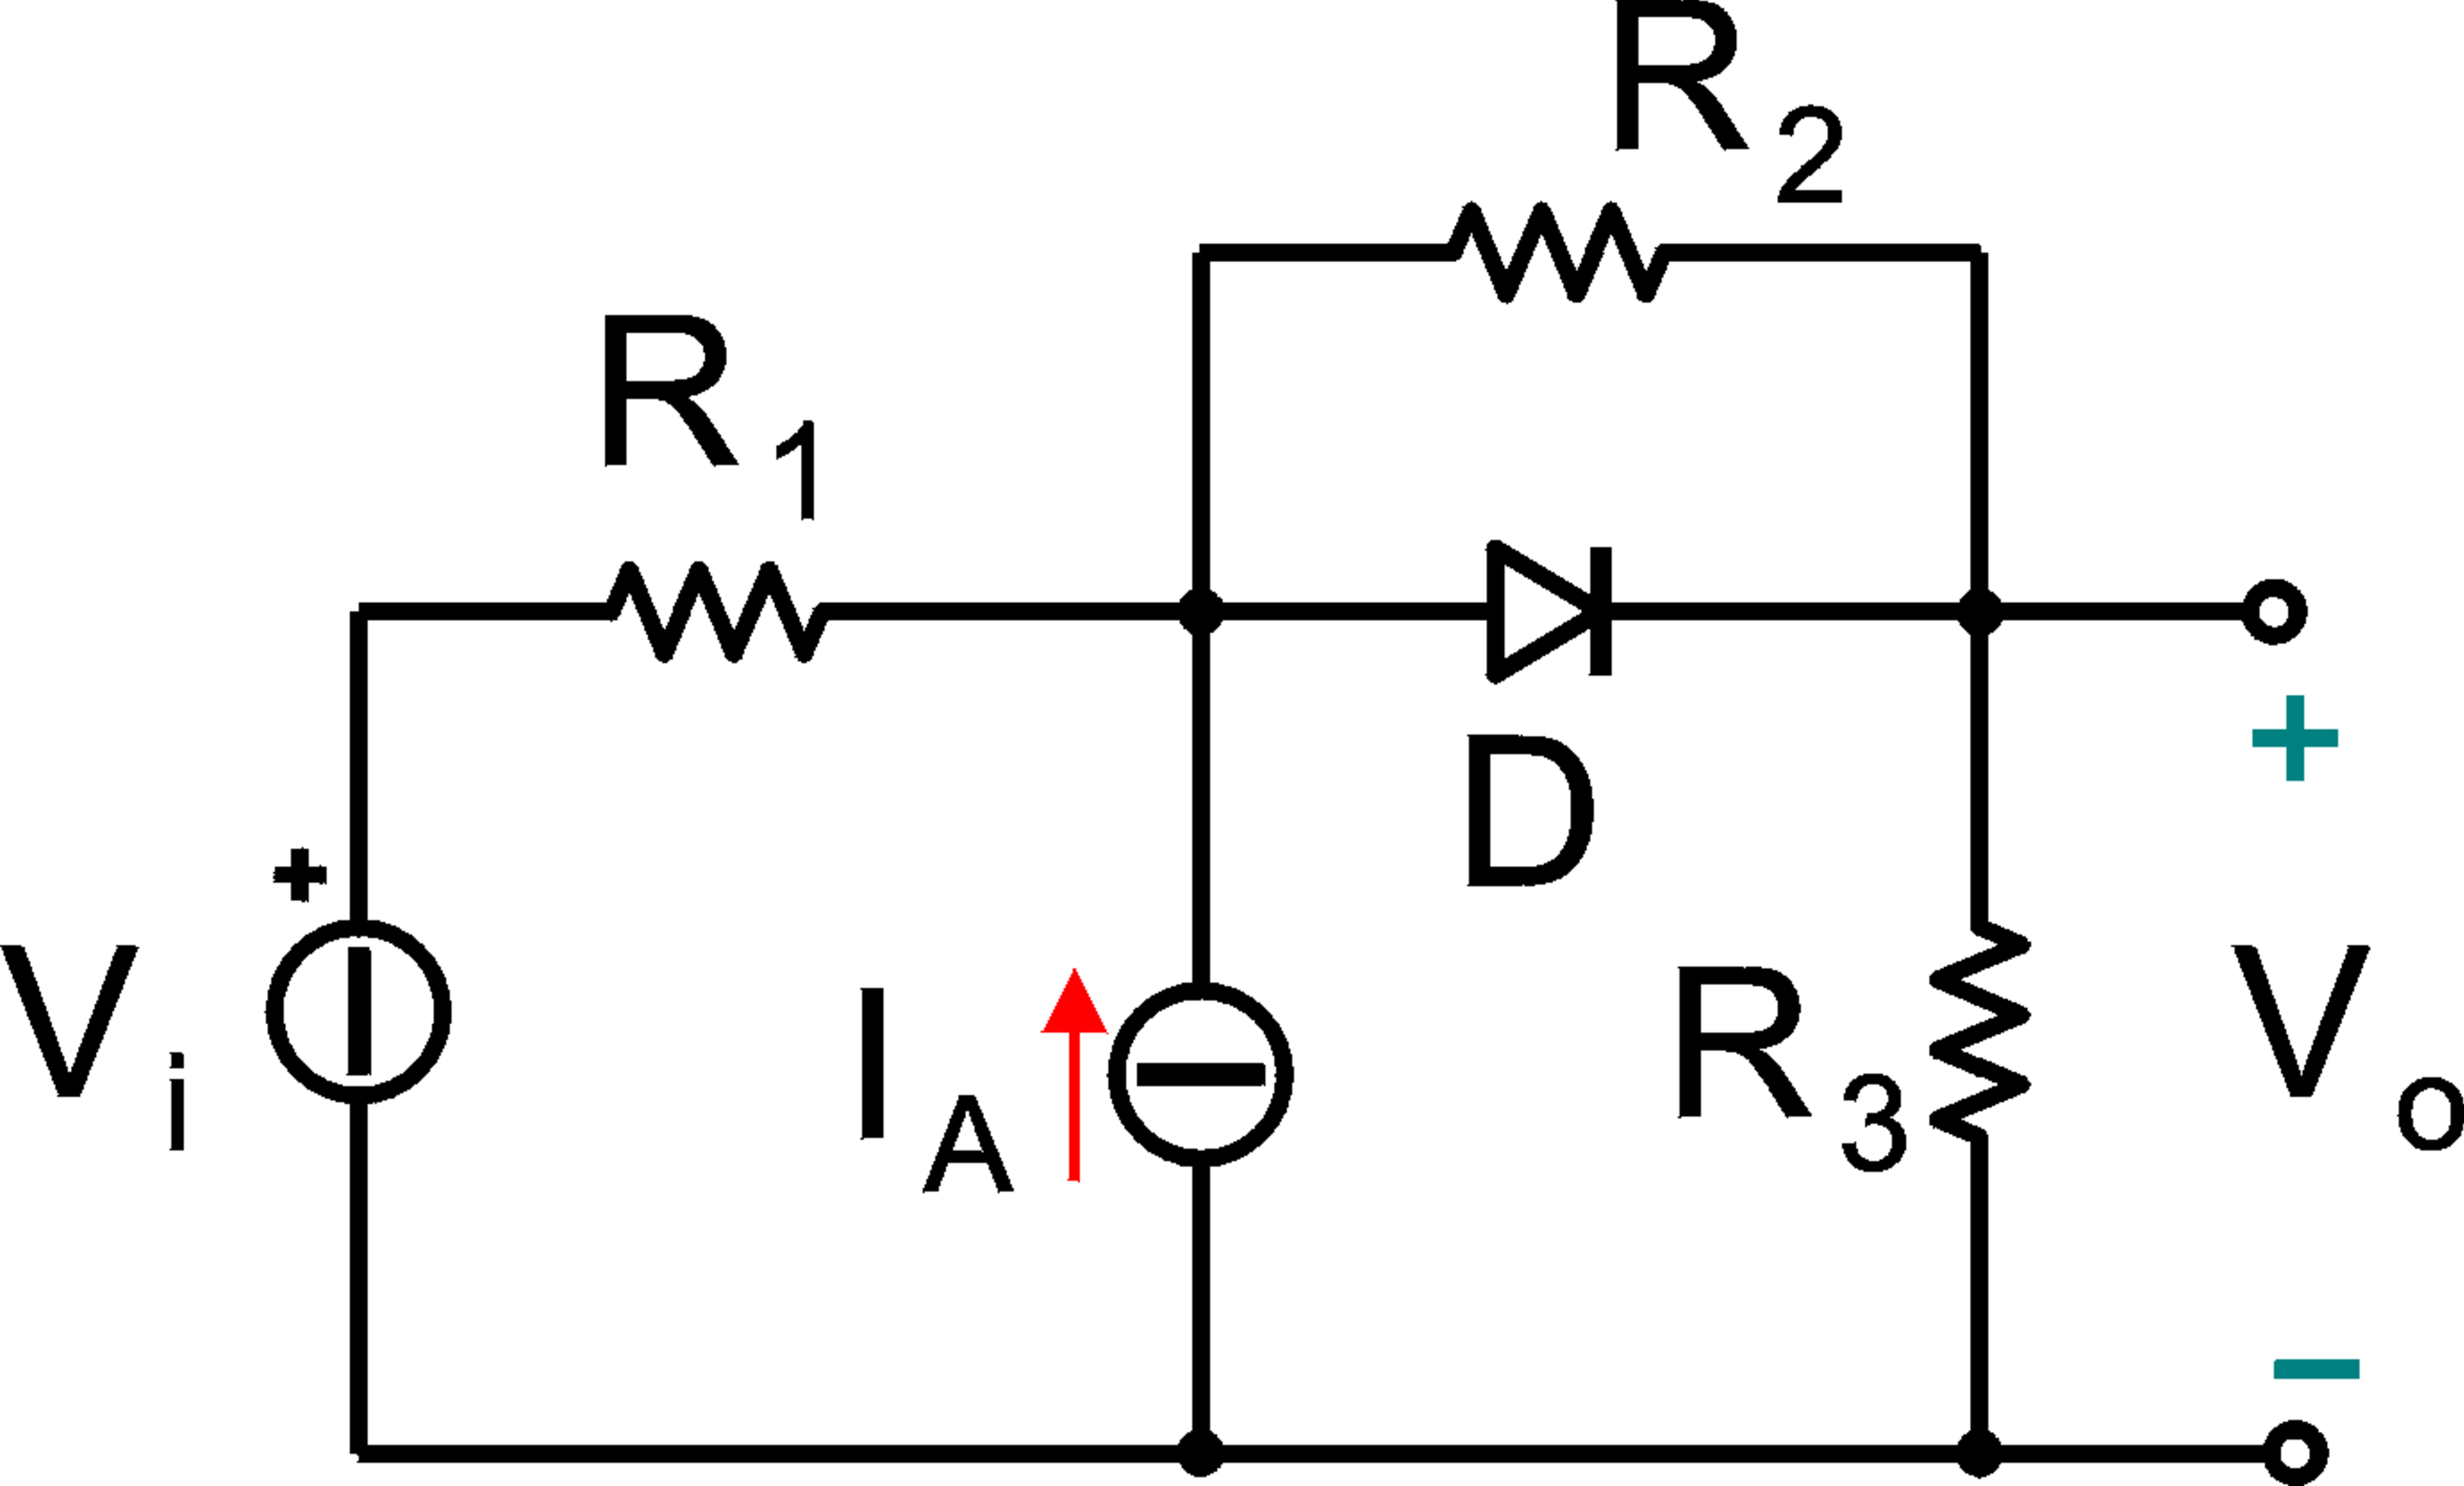
\includegraphics[width=.3\linewidth]{img/elettronicaEs/transdiodo1.pdf}
\caption{Trovare la transcaratteristica del circuito.}
\label{img:transdiodo1}
\end{figure}


\subsection{Esercizio}

Difficoltà: **\\

Il circuito di figura \ref{img:MOS1} rappresenta un transistore MOSFET a canale n polarizzato in zona di 
saturazione, con relativa transcaratteristica e retta di carico statica. Determinare, da tale grafico, i 
valori della resistenza di source $R_S$ e della tensione di alimentazione $V_{DD}$.\\

Dati
\begin{itemize}
\item $R_1=400\,k\Omega$
\item $R_2=500\,k\Omega$
\end{itemize}

RISPOSTE: $R_S = 150\,\Omega$, $V_{DD} = 9,9\,V$

\begin{figure}[H]
\centering
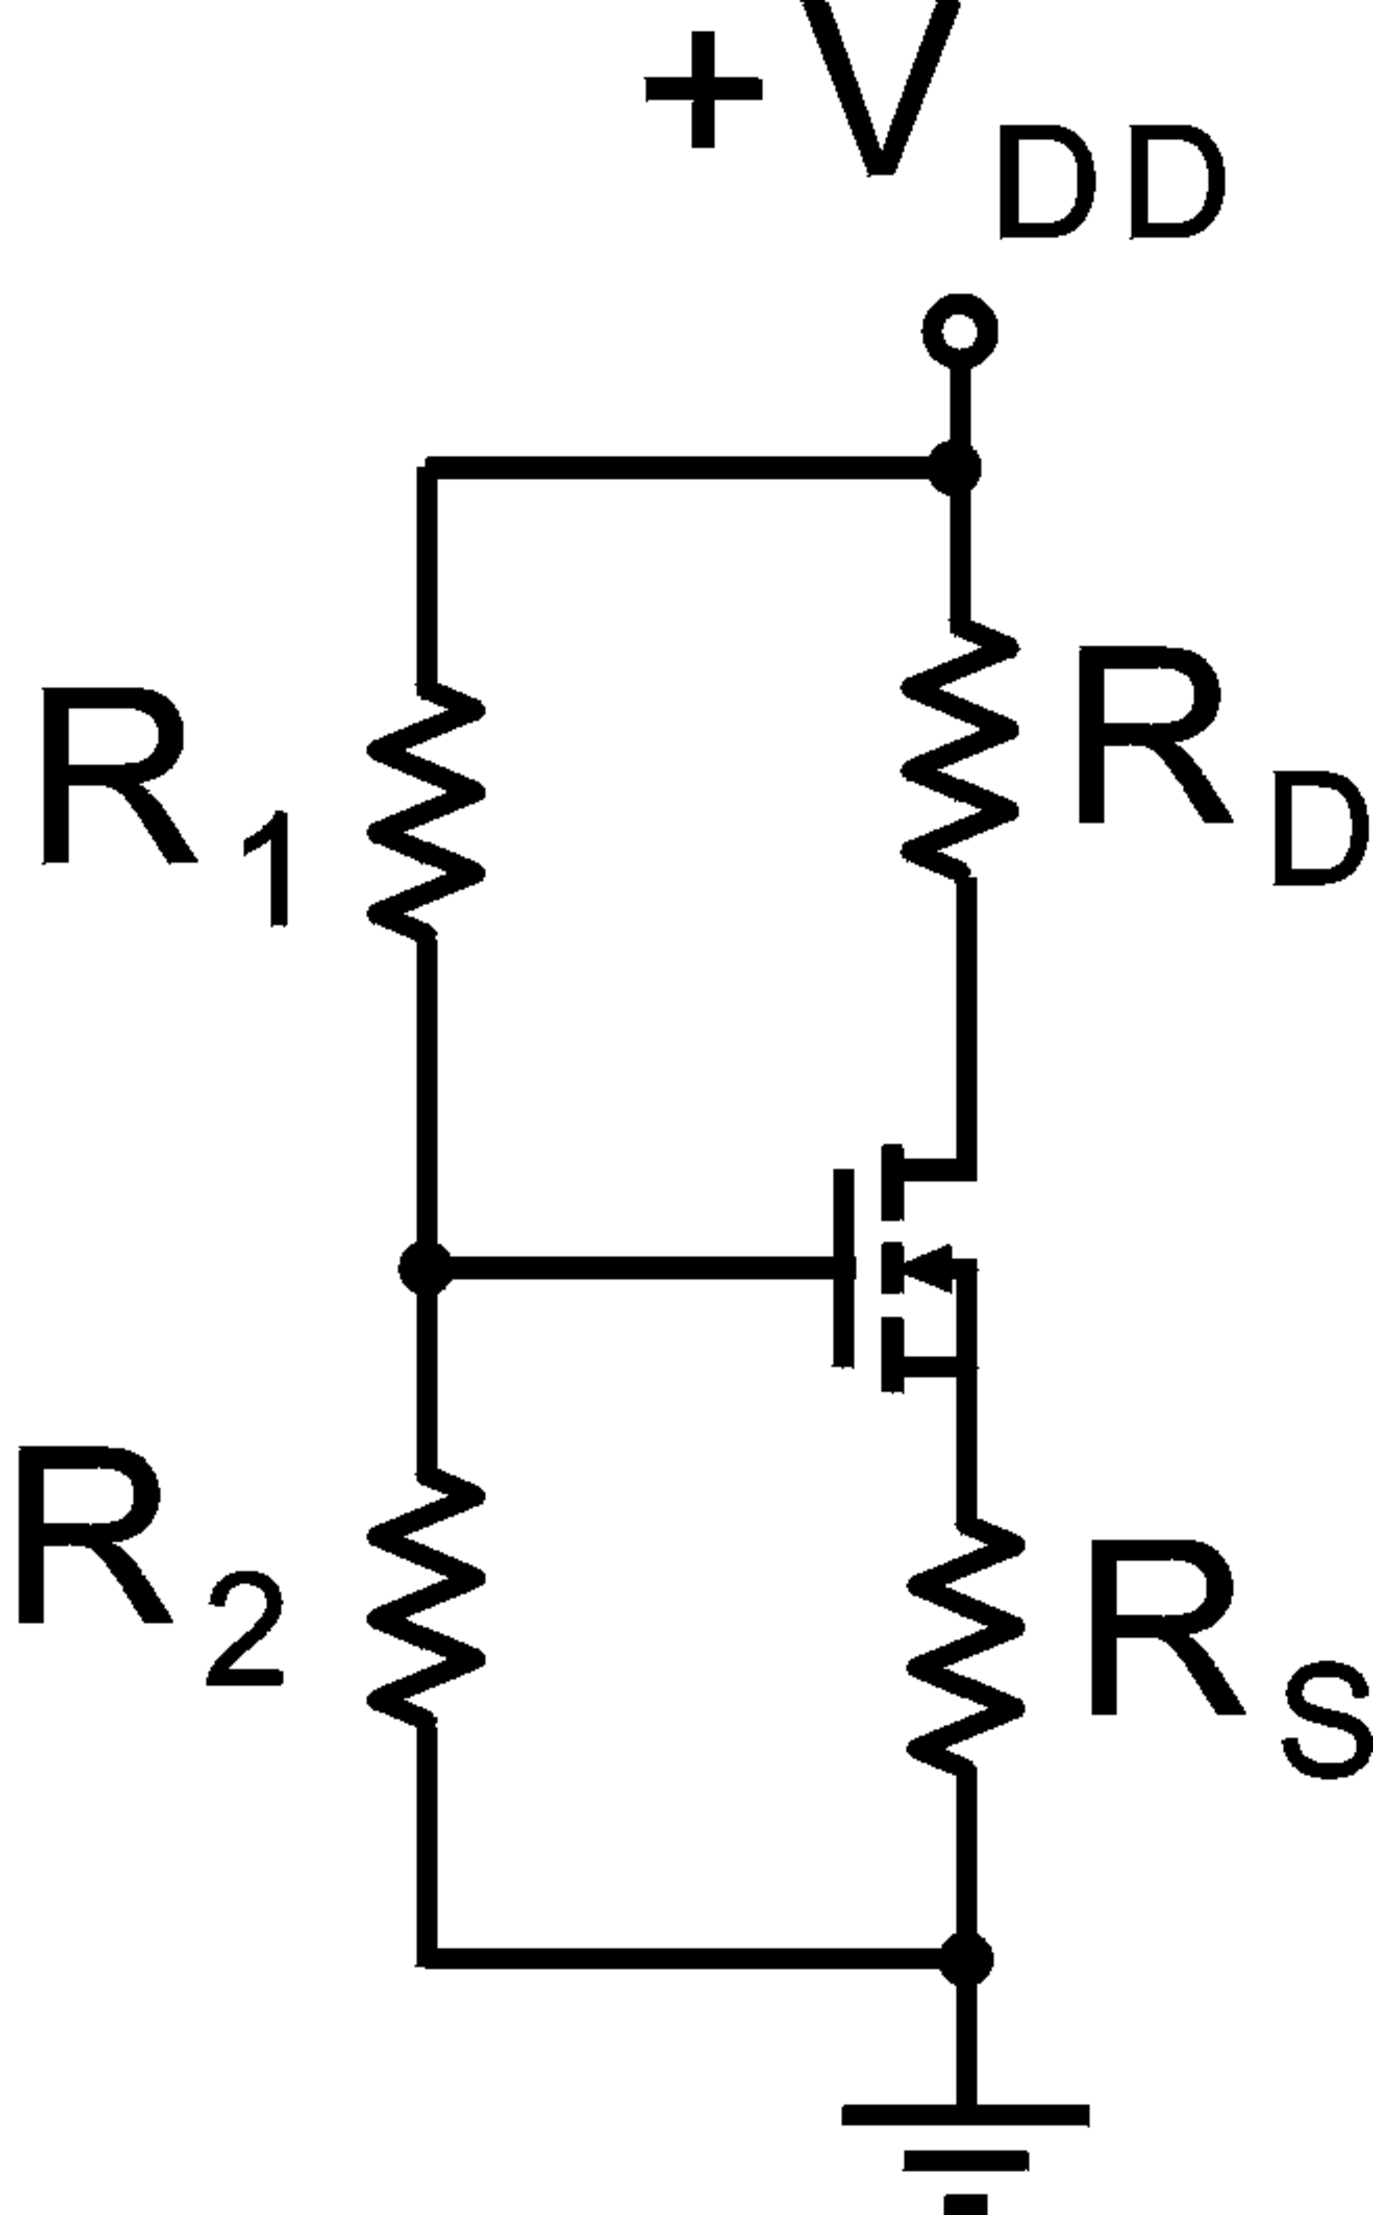
\includegraphics[width=.2\linewidth]{img/elettronicaEs/MOS1.pdf}
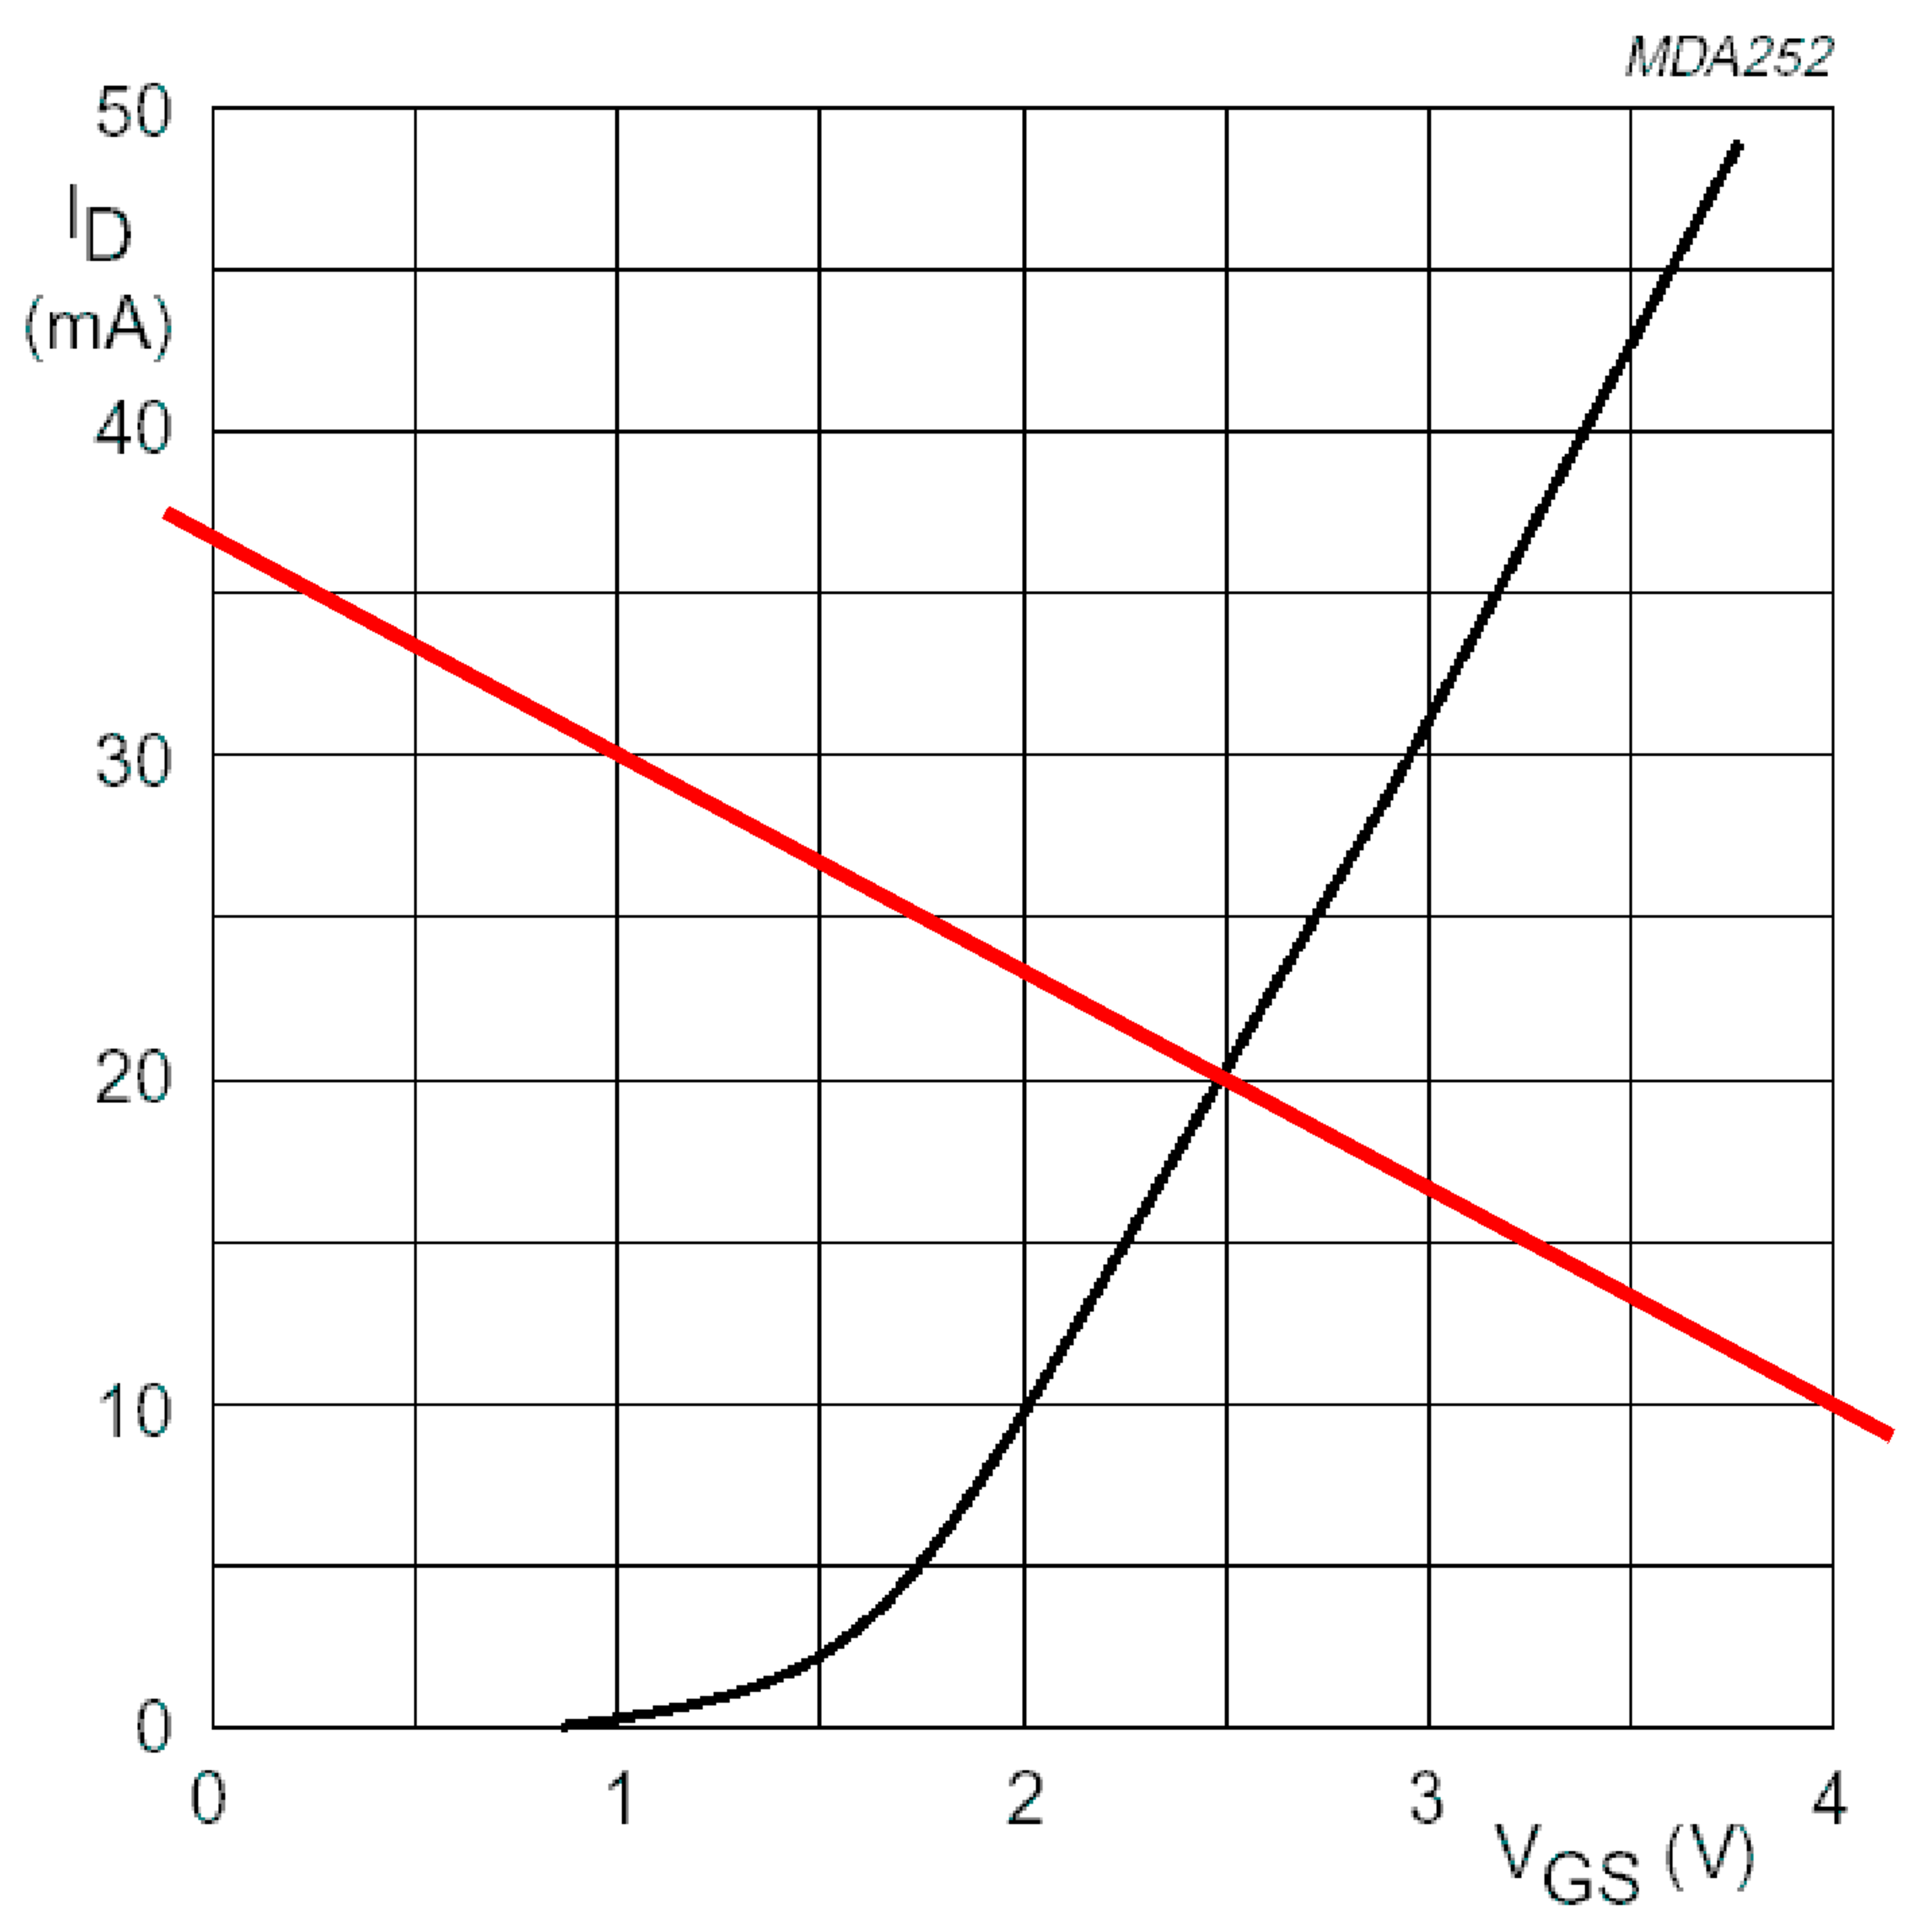
\includegraphics[width=.3\linewidth]{img/elettronicaEs/VGS.pdf}
\caption{Circuito di polarizzazione con MOSFET e relativa transcaratteristica e retta di carico.}
\label{img:MOS1}
\end{figure}


\subsection{Esercizio}

Difficoltà: **\\

Dato il circuito di figura \ref{img:MOS2}, determinare il valore della tensione gate-source 
$V_{GS}$ a riposo.\\

RISPOSTE: $V_{GS} = 7,85\,V$

Dati
\begin{itemize}
\item $R_G=40\,k\Omega$ 
\item $R_D=2200\,\Omega$
\item $V_{DD}=15\,V$ 
\item $V_T=5\,V$
\item $I_{DSS}=V_T2\mu C_{ox}{W\over 2L}=10\,mA$
\end{itemize}

\begin{figure}[H]
\centering
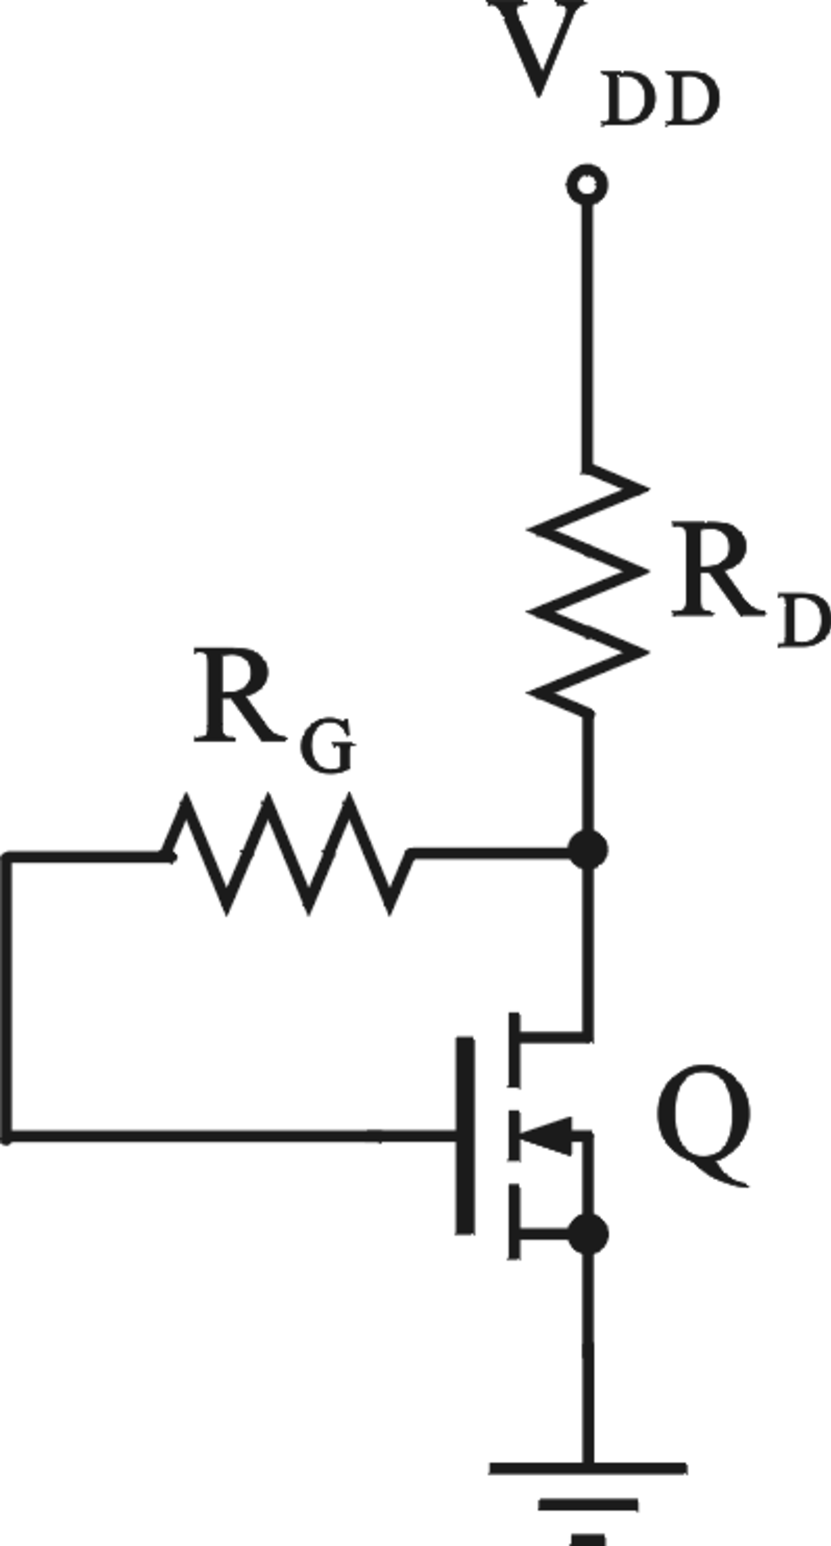
\includegraphics[width=.2\linewidth]{img/elettronicaEs/MOS2.pdf}
\caption{Circuito di polarizzazione con MOSFET.}
\label{img:MOS2}
\end{figure}


\subsection{Esercizio}

Difficoltà: **\\

Nel circuito di figura \ref{img:filtrointegratore} $R = 1\,k\Omega$, $C=1\,\mu F$. Qual'è il valore in modulo 
dell'amplificazione di tensione alla frequenza angolare $\omega_0$ di $120\,rad/s$?\\

RISPOSTA: $\left|A_v(\omega_0)\right| = 8,33$


\subsection{Esercizio}

Difficoltà: **\\

Nel circuito di figura \ref{img:filtrointegratore}, che usa un amplificatore operazionale ideale, $R = 10\, 
k\Omega$, $C = 10\,nF$. Determinare il valore (in Volt) cui si porta la tensione di uscita dopo $1\,ms$, se 
all'ingresso è applicata una tensione $V_I = 1\,V$. Si supponga la capacità $C$ inizialmente scarica.\\

RISPOSTA: $v_o(1\,ms) = -10\,V$


\subsection{Esercizio}

Difficoltà: **\\

Nel circuito di figura \ref{img:filtrointegratore}, che usa un amplificatore operazionale ideale, 
$R = 33\,k\Omega$, $C = 10\,nF$. Determinare il tempo $t_r$ (in $ms$) richiesto affinchè l'uscita si porti 
ad una tensione di $12\,V$, se all'ingresso è applicata una tensione $V_I = -2\,V$. Si supponga la capacità 
$C$ inizialmente scarica.\\

RISPOSTA: $1,98\,ms$.

\begin{figure}[H]
\centering
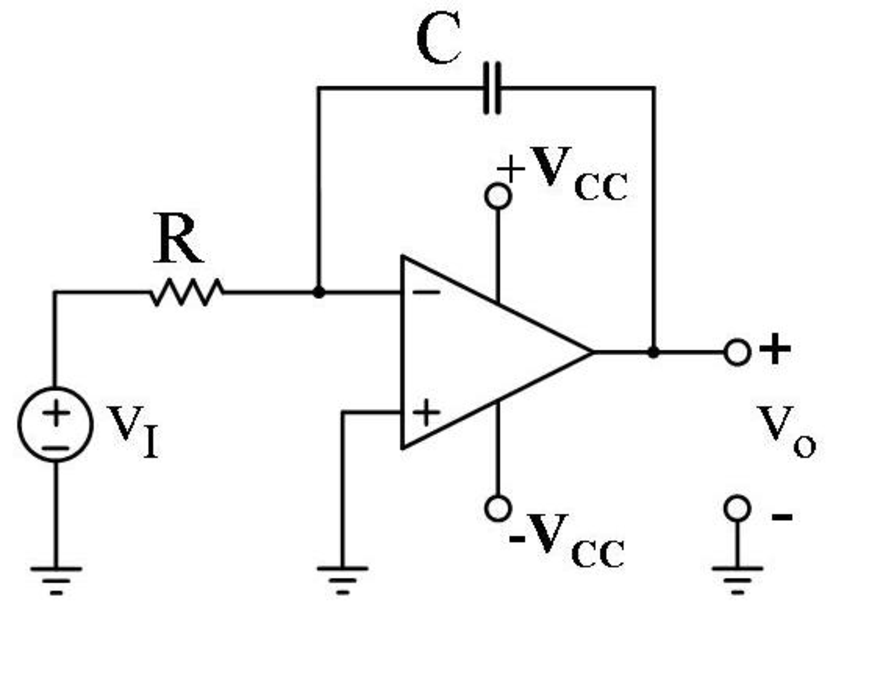
\includegraphics[width=.3\linewidth]{img/elettronicaEs/filtrointegratore.pdf}
\caption{Filtro integratore.}
\label{img:filtrointegratore}
\end{figure}


\subsection{Esercizio}

Difficoltà: ***\\

Dato il raddrizzatore ad una semionda riportato in figura \ref{img:raddrizzatore} con carico resistivo e 
filtro capacitivo, determinare la durata dell'intervallo di conduzione $T_c$ del diodo ed il valore di 
picco $I_{pk}$ della corrente nel diodo a regime. Si consideri ideale il diodo.\\

Dati
\begin{itemize}
\item $R_L=100\,\Omega$ 
\item $C=2000\,\mu F$ 
\item $V_p=150\,V$
\item $\omega = 314\,rad/s$
\end{itemize}

RISPOSTE: $T_c = 1,42\,ms$, $I_{pk} = 42,14\,A$


\subsection{Esercizio}

Difficoltà: ***\\

Dato il raddrizzatore ad una semionda riportato in figura \ref{img:raddrizzatore} con carico resistivo e 
filtro capacitivo, determinare il valore della resistenza di carico $R_L$ per avere una tensione di 
ondulazione (ripple voltage) $V_r$ pari al del $30\%$ della tensione a vuoto (cioè, con $R_L$ infinita). 
Determinare, inoltre, il valore di picco $I_{pk}$ della corrente nel diodo a regime nel caso in cui la 
resistenza di carico sia di $80\,\Omega$.\\

Dati
\begin{itemize}
\item $C=1200\,\mu F$ 
\item $V_p=50\,V$ 
\item $\omega=314\,rad/s$
\end{itemize}

RISPOSTE: $R = 55,58\,\Omega$, $I_{pk} = 12,17\,A$


\subsection{Esercizio}

Difficoltà: ***\\

Dato il raddrizzatore ad una semionda riportato in figura \ref{img:raddrizzatore} con carico resistivo e 
filtro capacitivo, determinare il valore della capacità di filtro $C$ per avere una tensione media di uscita 
(definita come media aritmetica dei valori massimo e e minimo della tensione sul carico) di $34\,V$. 
Determinare, inoltre, la durata dell'intervallo di conduzione $T_c$ del diodo. Si consideri ideale il diodo.

Dati
\begin{itemize}
\item $R_L=200\,\Omega$
\item $V_p=40\,V$ 
\item $\omega=314rad/s$
\end{itemize}

RISPOSTE: $C=333,5\,\mu F$, $T_c = 2,46\,ms$

\begin{figure}[H]
\centering
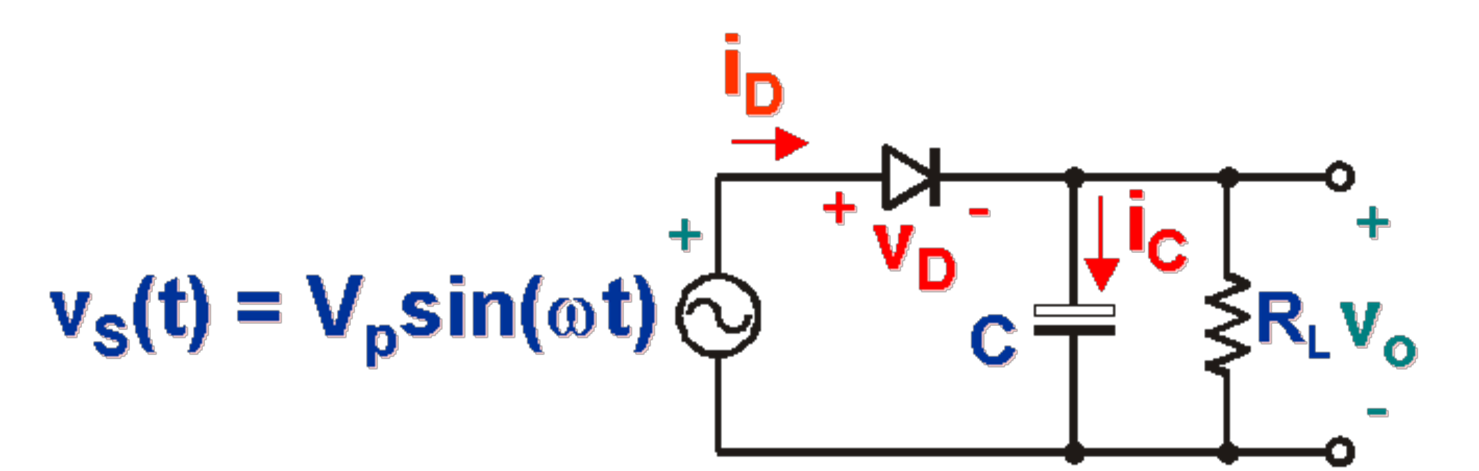
\includegraphics[width=.5\linewidth]{img/elettronicaEs/raddrizzatore.pdf}
\caption{Raddrizzatore a semionda.}
\label{img:raddrizzatore}
\end{figure}


\subsection{Esercizio}

Difficoltà: ***\\

Il circuito di figura \ref{img:EC}, rappresenta un amplificatore a singolo transistore che lavora a 
temperatura ambiente ($T_A = 25^{\circ}C$). Dopo aver disegnato il circuito dinamico equivalente e 
trascurando l'effetto Early, si determini:
\begin{enumerate}
\item la resistenza d'ingresso $R_{in}$ (la resistenza d'ingresso vista dal generatore di sorgente reale 
	cioè a valle della resistenza $R_g$);
\item il guadagno di tensione complessivo $A_v$ (il rapporto tra la tensione di uscita $v_o$ e la tensione 
	$v_g$ del generatore di segnale);
\item la potenza $P_A$ erogata dal generatore di corrente $I_A$.
\end{enumerate}

Dati
\begin{itemize}
\item $I_A = 1,5\,mA$
\item $V_{CC}=-5\,V$
\item $V_{EE}=-12\,V$ 
\item $R_1=330\,k\Omega$
\item $R_g=20\,k\Omega$
\item $R_L=18k\Omega$
\item $\beta_F=100$
\item $\beta_0=120$
\end{itemize}

RISPOSTE: $R_{in} = k\Omega$, $A_v = $, $P_A = mW$

\begin{figure}[H]
\centering
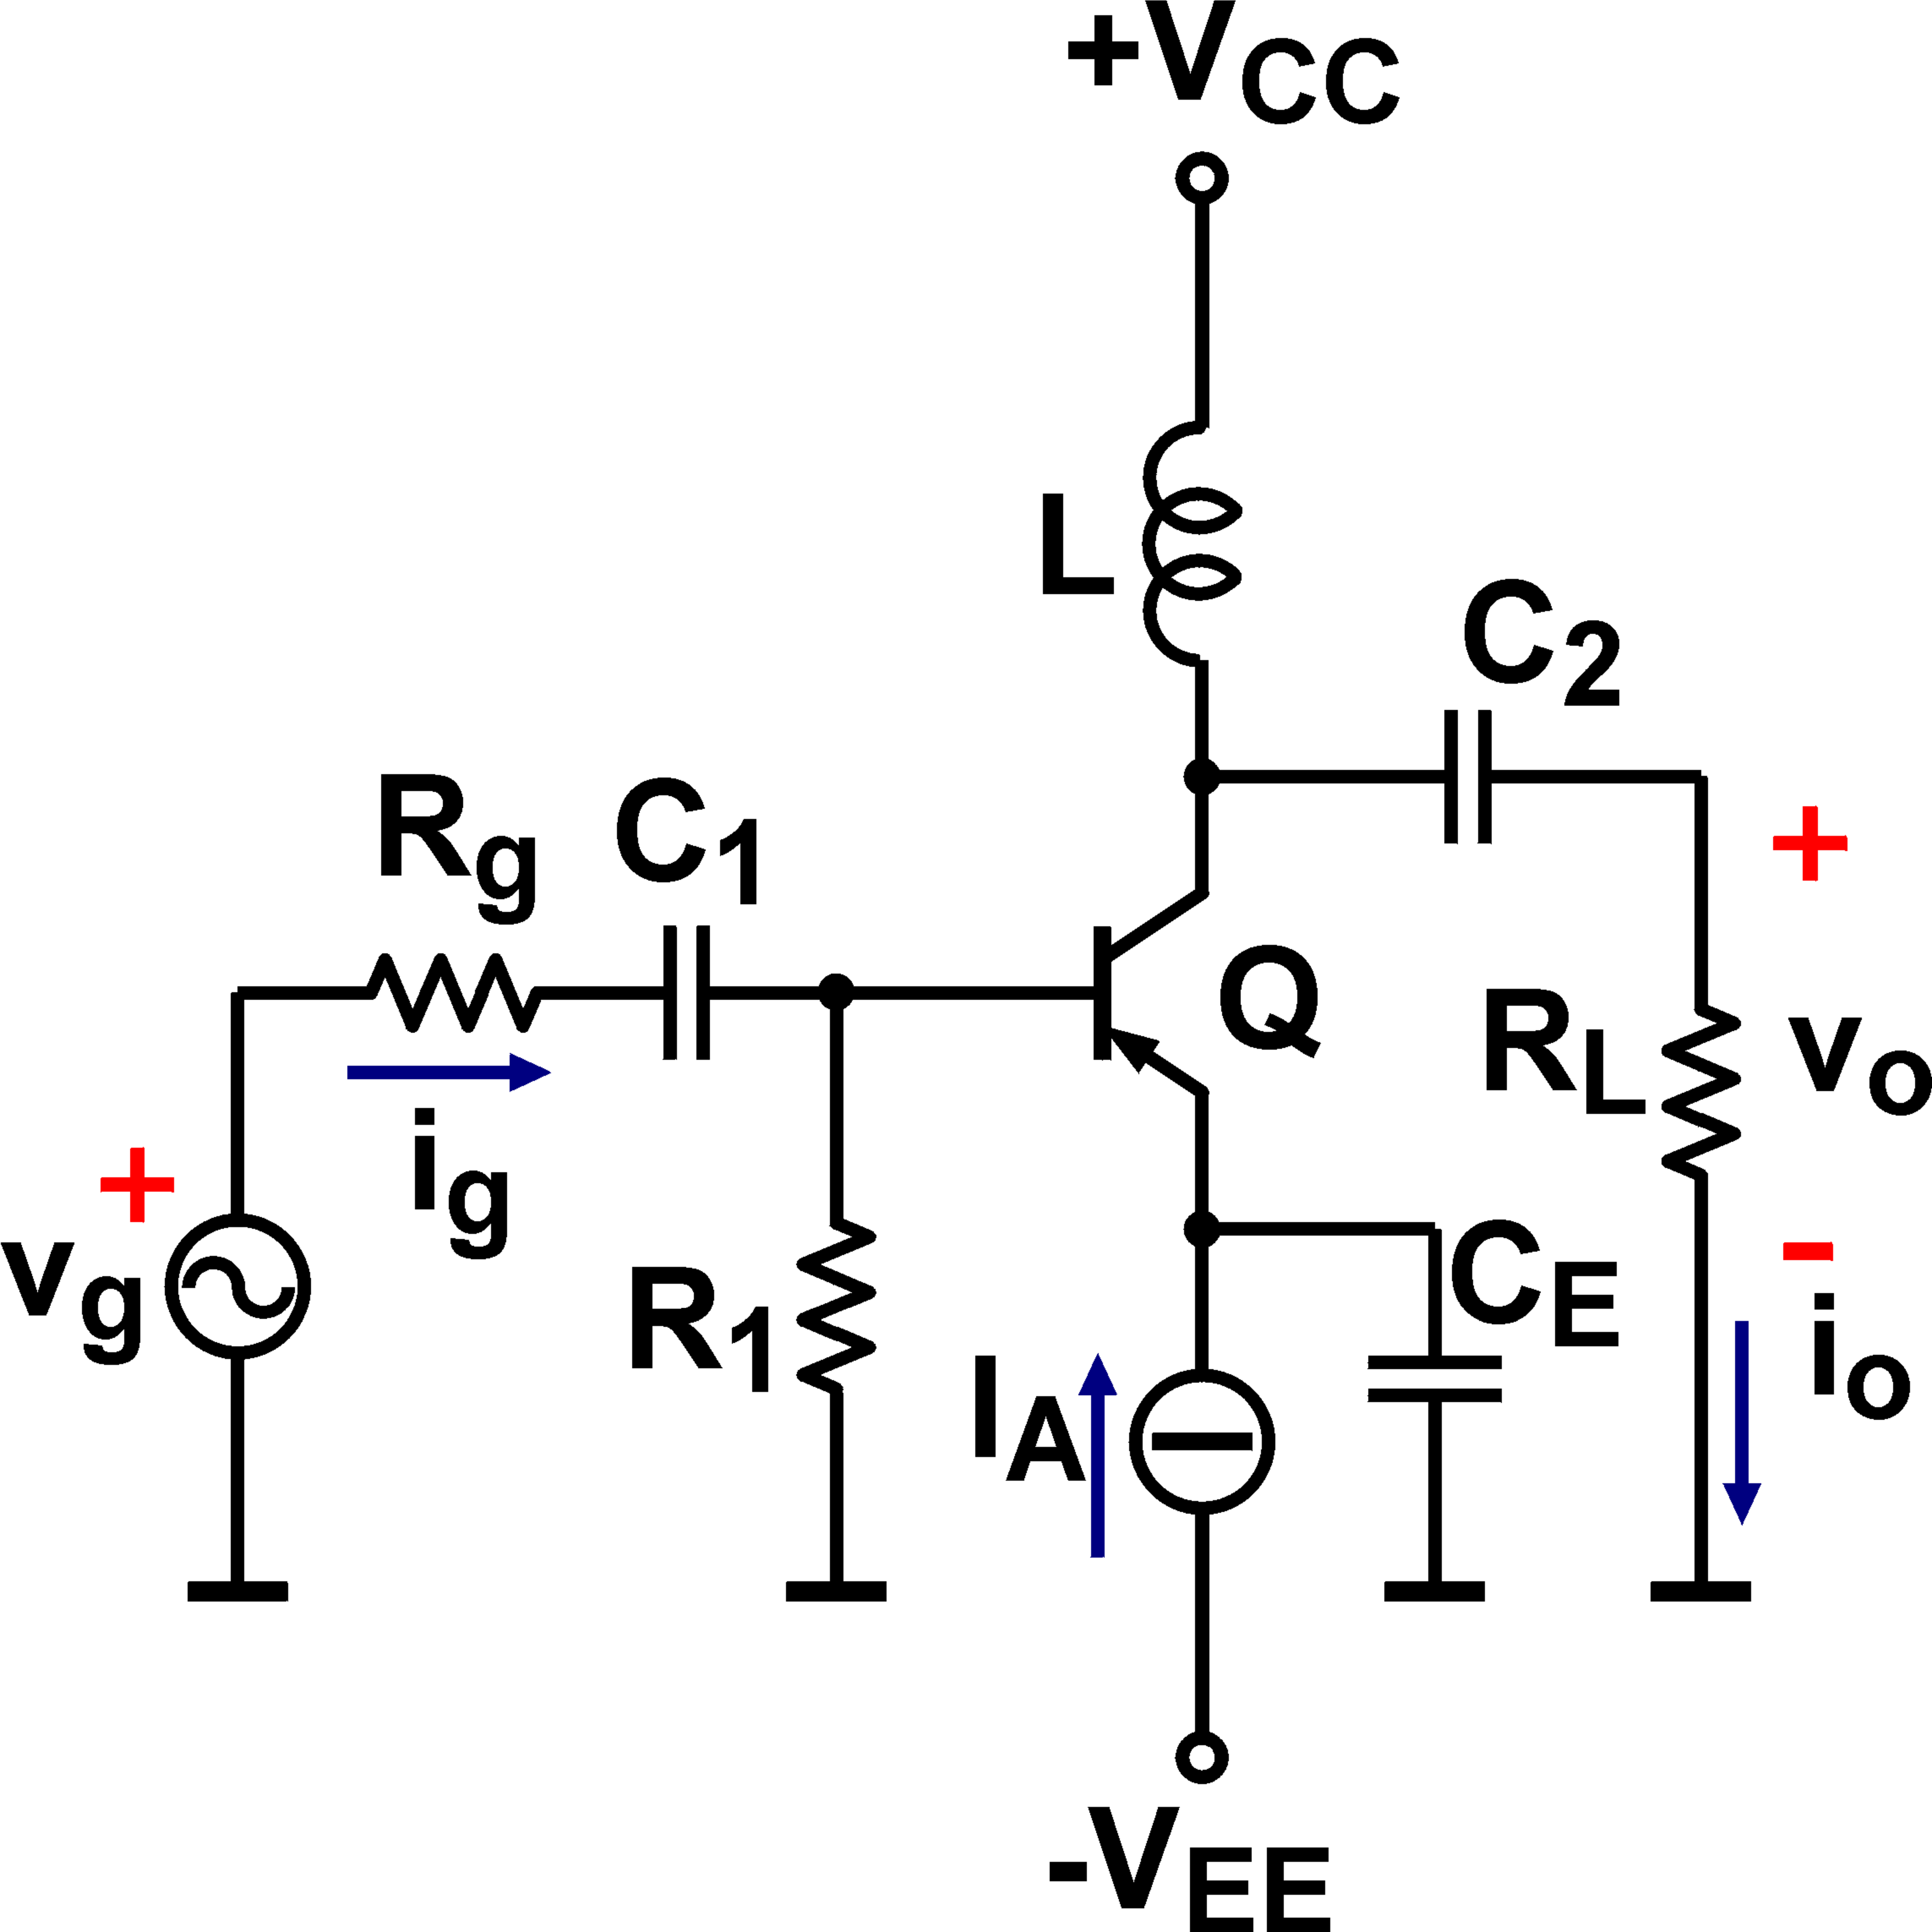
\includegraphics[width=.5\linewidth]{img/elettronicaEs/EC.pdf}
\caption{Schema BJT a emettitore comune.}
\label{img:EC}
\end{figure}


\subsection{Esercizio}

Difficoltà: ***\\

Il circuito di figura \ref{img:CC} rappresenta un amplificatore a singolo transistore che lavora a 
temperatura ambiente ($T_A = 25^{\circ}C$). Dopo aver disegnato il circuito dinamico equivalente valido a 
centro banda, e trascurando l'effetto Early, si determini:
\begin{enumerate}
\item la resistenza d'ingresso intrinseca $R_i$ (la resistenza d'ingresso vista tra Base e Massa nel circuito 
	dinamico equivalente);
\item il guadagno di tensione intrinseco $A_{vt}$ (il rapporto tra la tensione di uscita $v_o$ e la tensione 
	tra Base e Massa nel circuito dinamico equivalente);
\item l'attenuazione d'ingresso $\alpha$ (il rapporto tra la tensione tra Base e Massa nel circuito dinamico 
	equivalente e la tensione del generatore di segnale $v_g$).
\end{enumerate}

Dati
\begin{itemize}
\item $R_1=330\,k\Omega$ 
\item $R_g=10\,k\Omega$
\item $R_E=4.7\,k\Omega$
\item $R_L=1\,k\Omega$
\item $I_{CQ}=0.41\,mA$
\item $\beta_0=200$
\end{itemize}

RISPOSTE: $R_i = 177,9\,k\Omega$, $A_{vt} = 0,93$, $\alpha = 0,92$

\begin{figure}[H]
\centering
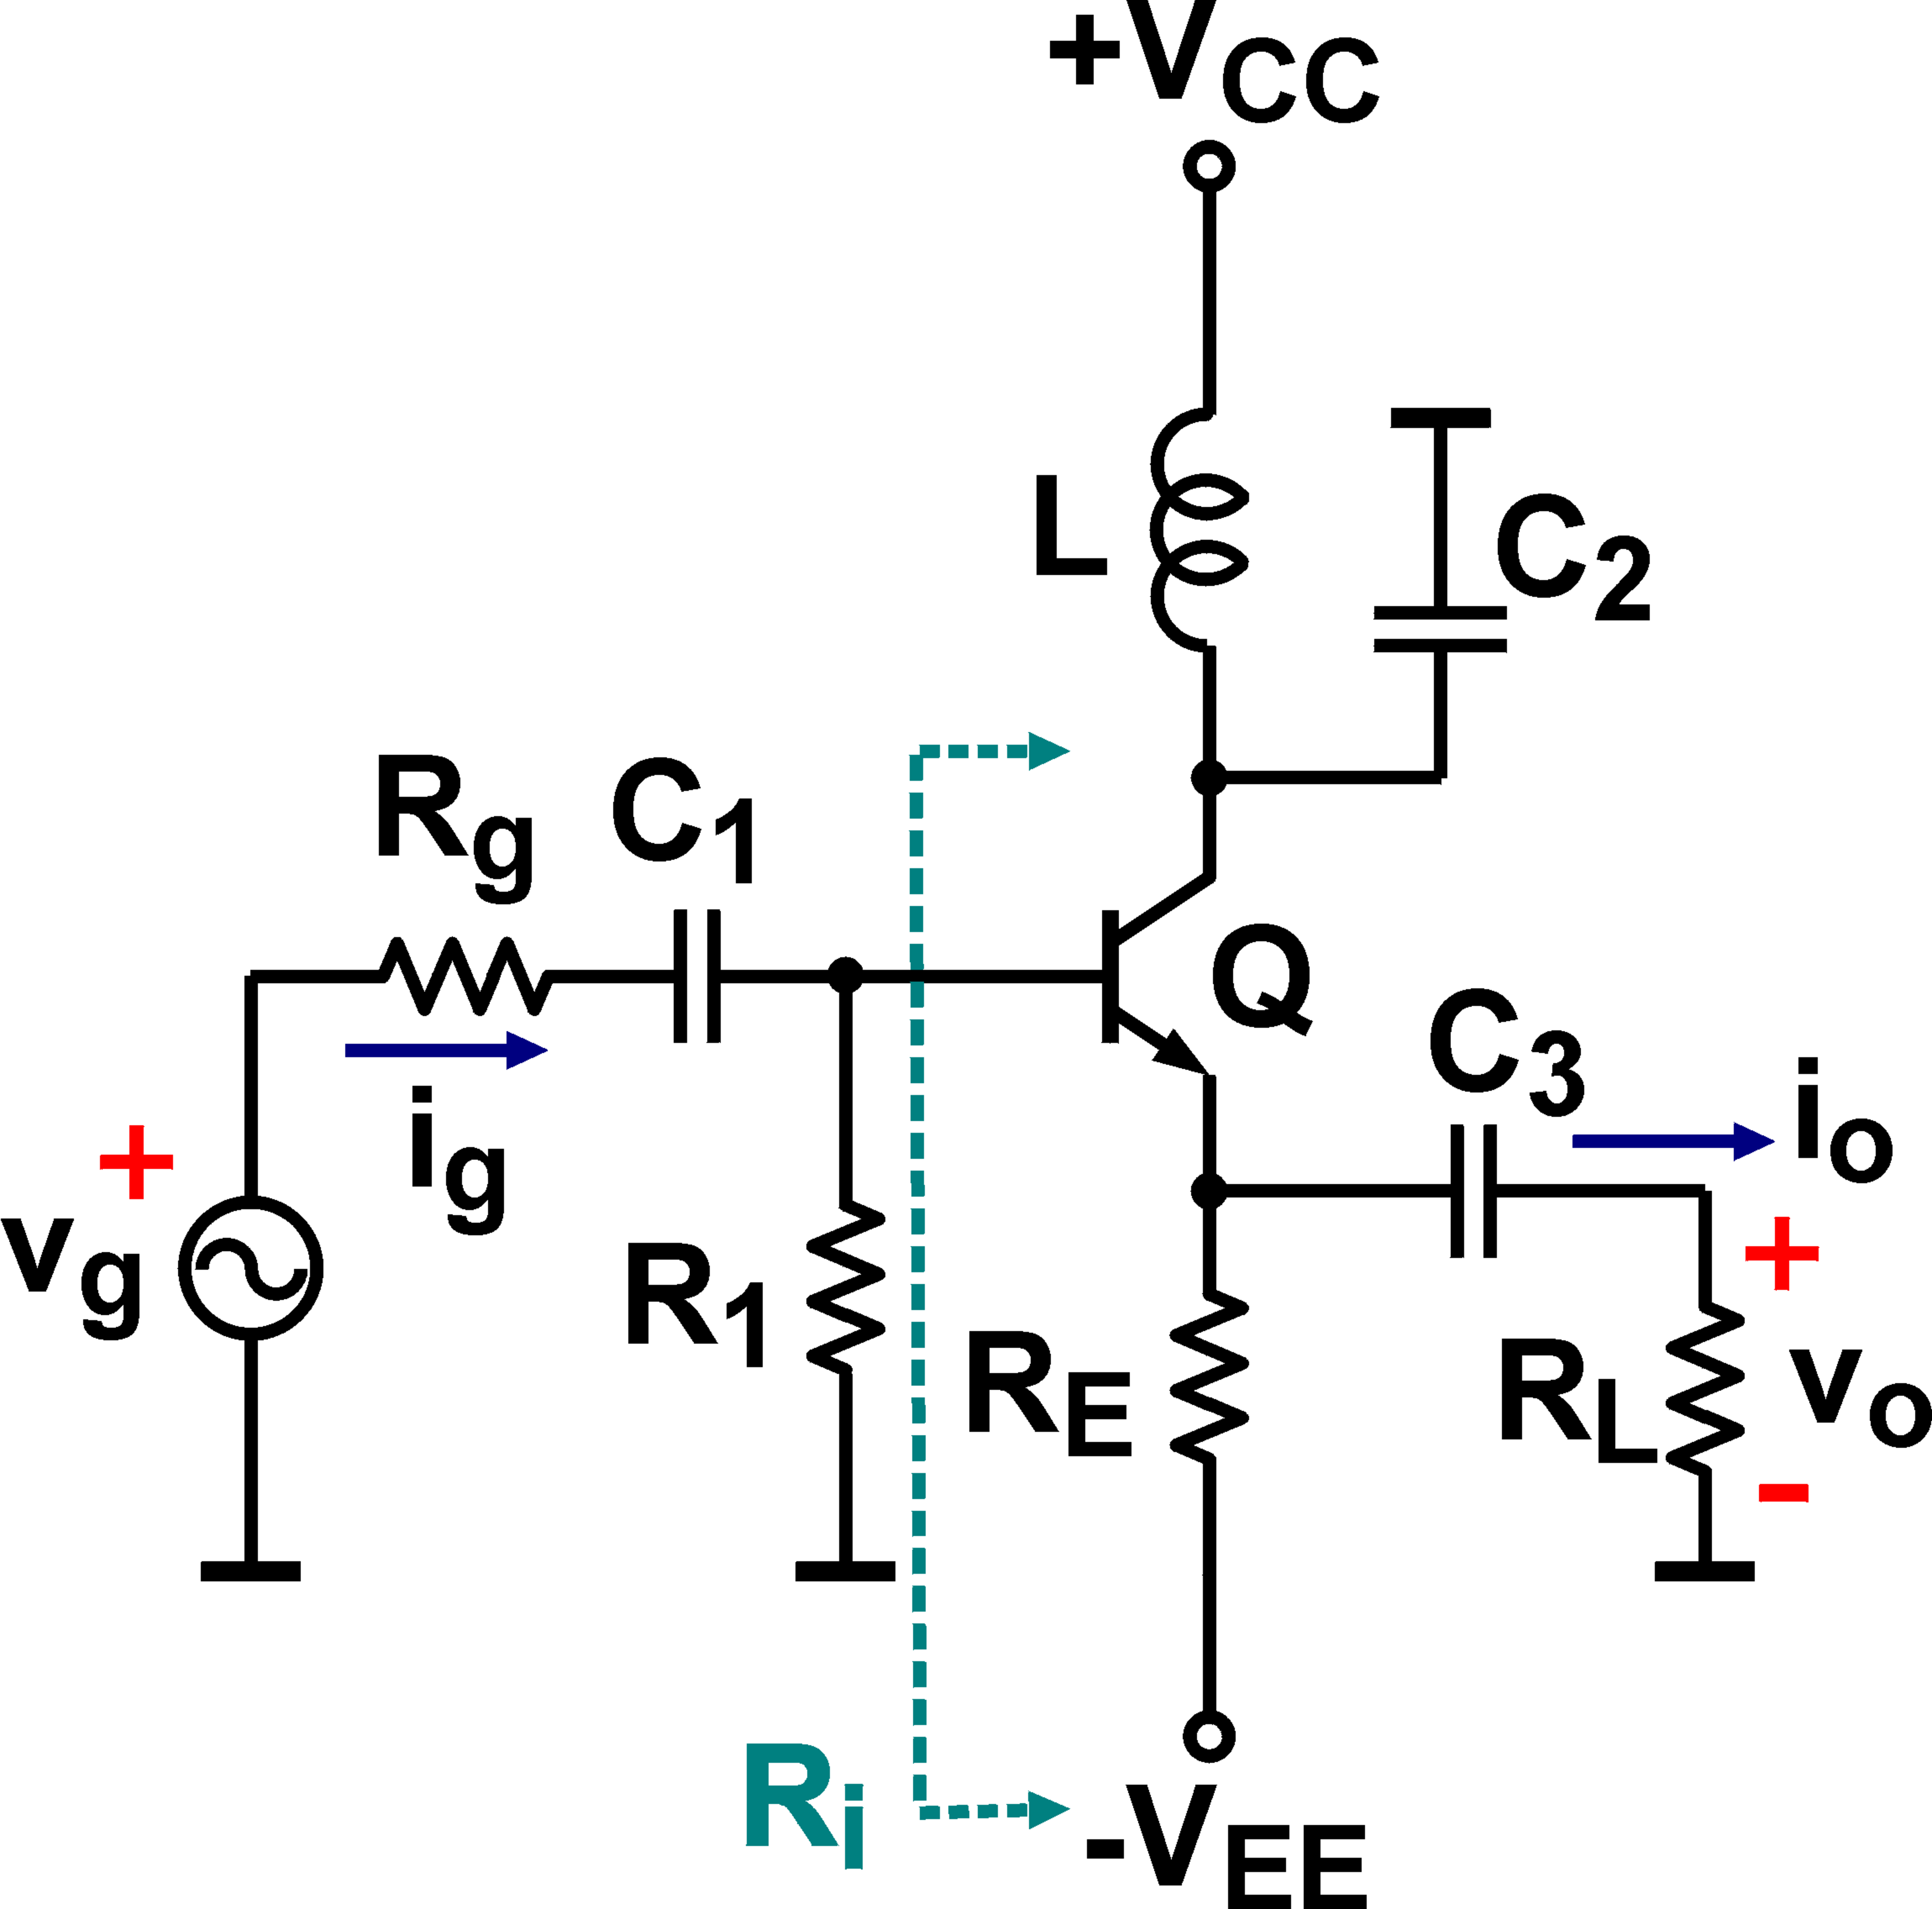
\includegraphics[width=.5\linewidth]{img/elettronicaEs/CC.pdf}
\caption{Schema BJT a collettore comune.}
\label{img:CC}
\end{figure}


\subsection{Esercizio}

Difficoltà: **\\

Dato il circuito di figura \ref{img:trasferimento}, che utilizza un amplificatore operazionale ideale, 
determinare la funzione di trasferimento tra $V_{in}$ e $V_o$ scegliendo tra quelle in figura.\\

RISPOSTA: a

\begin{figure}[H]
\centering
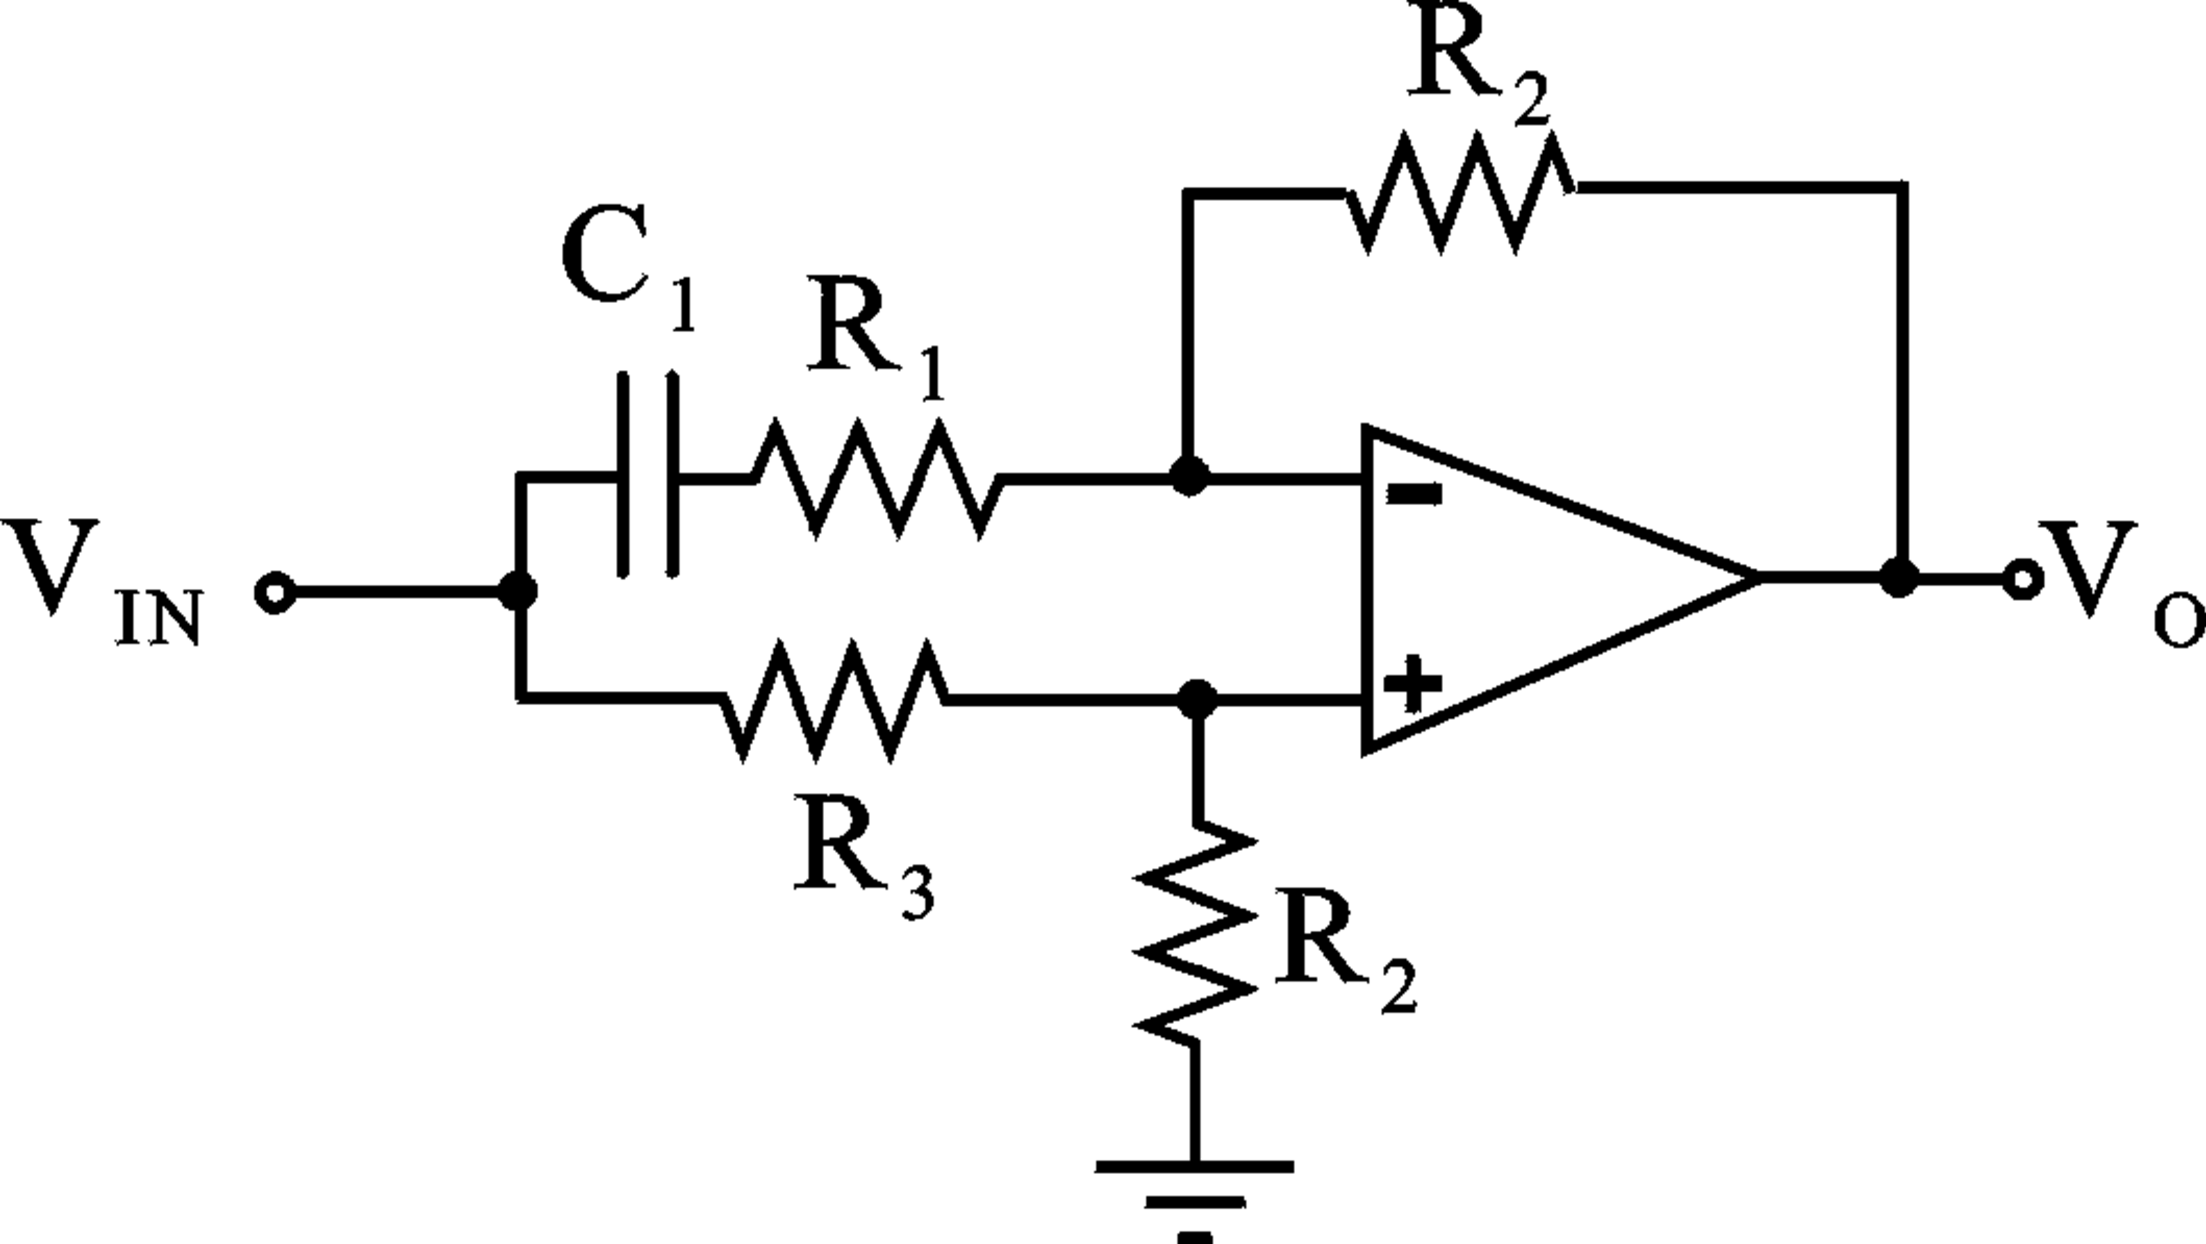
\includegraphics[width=.3\linewidth]{img/elettronicaEs/ampli.pdf}
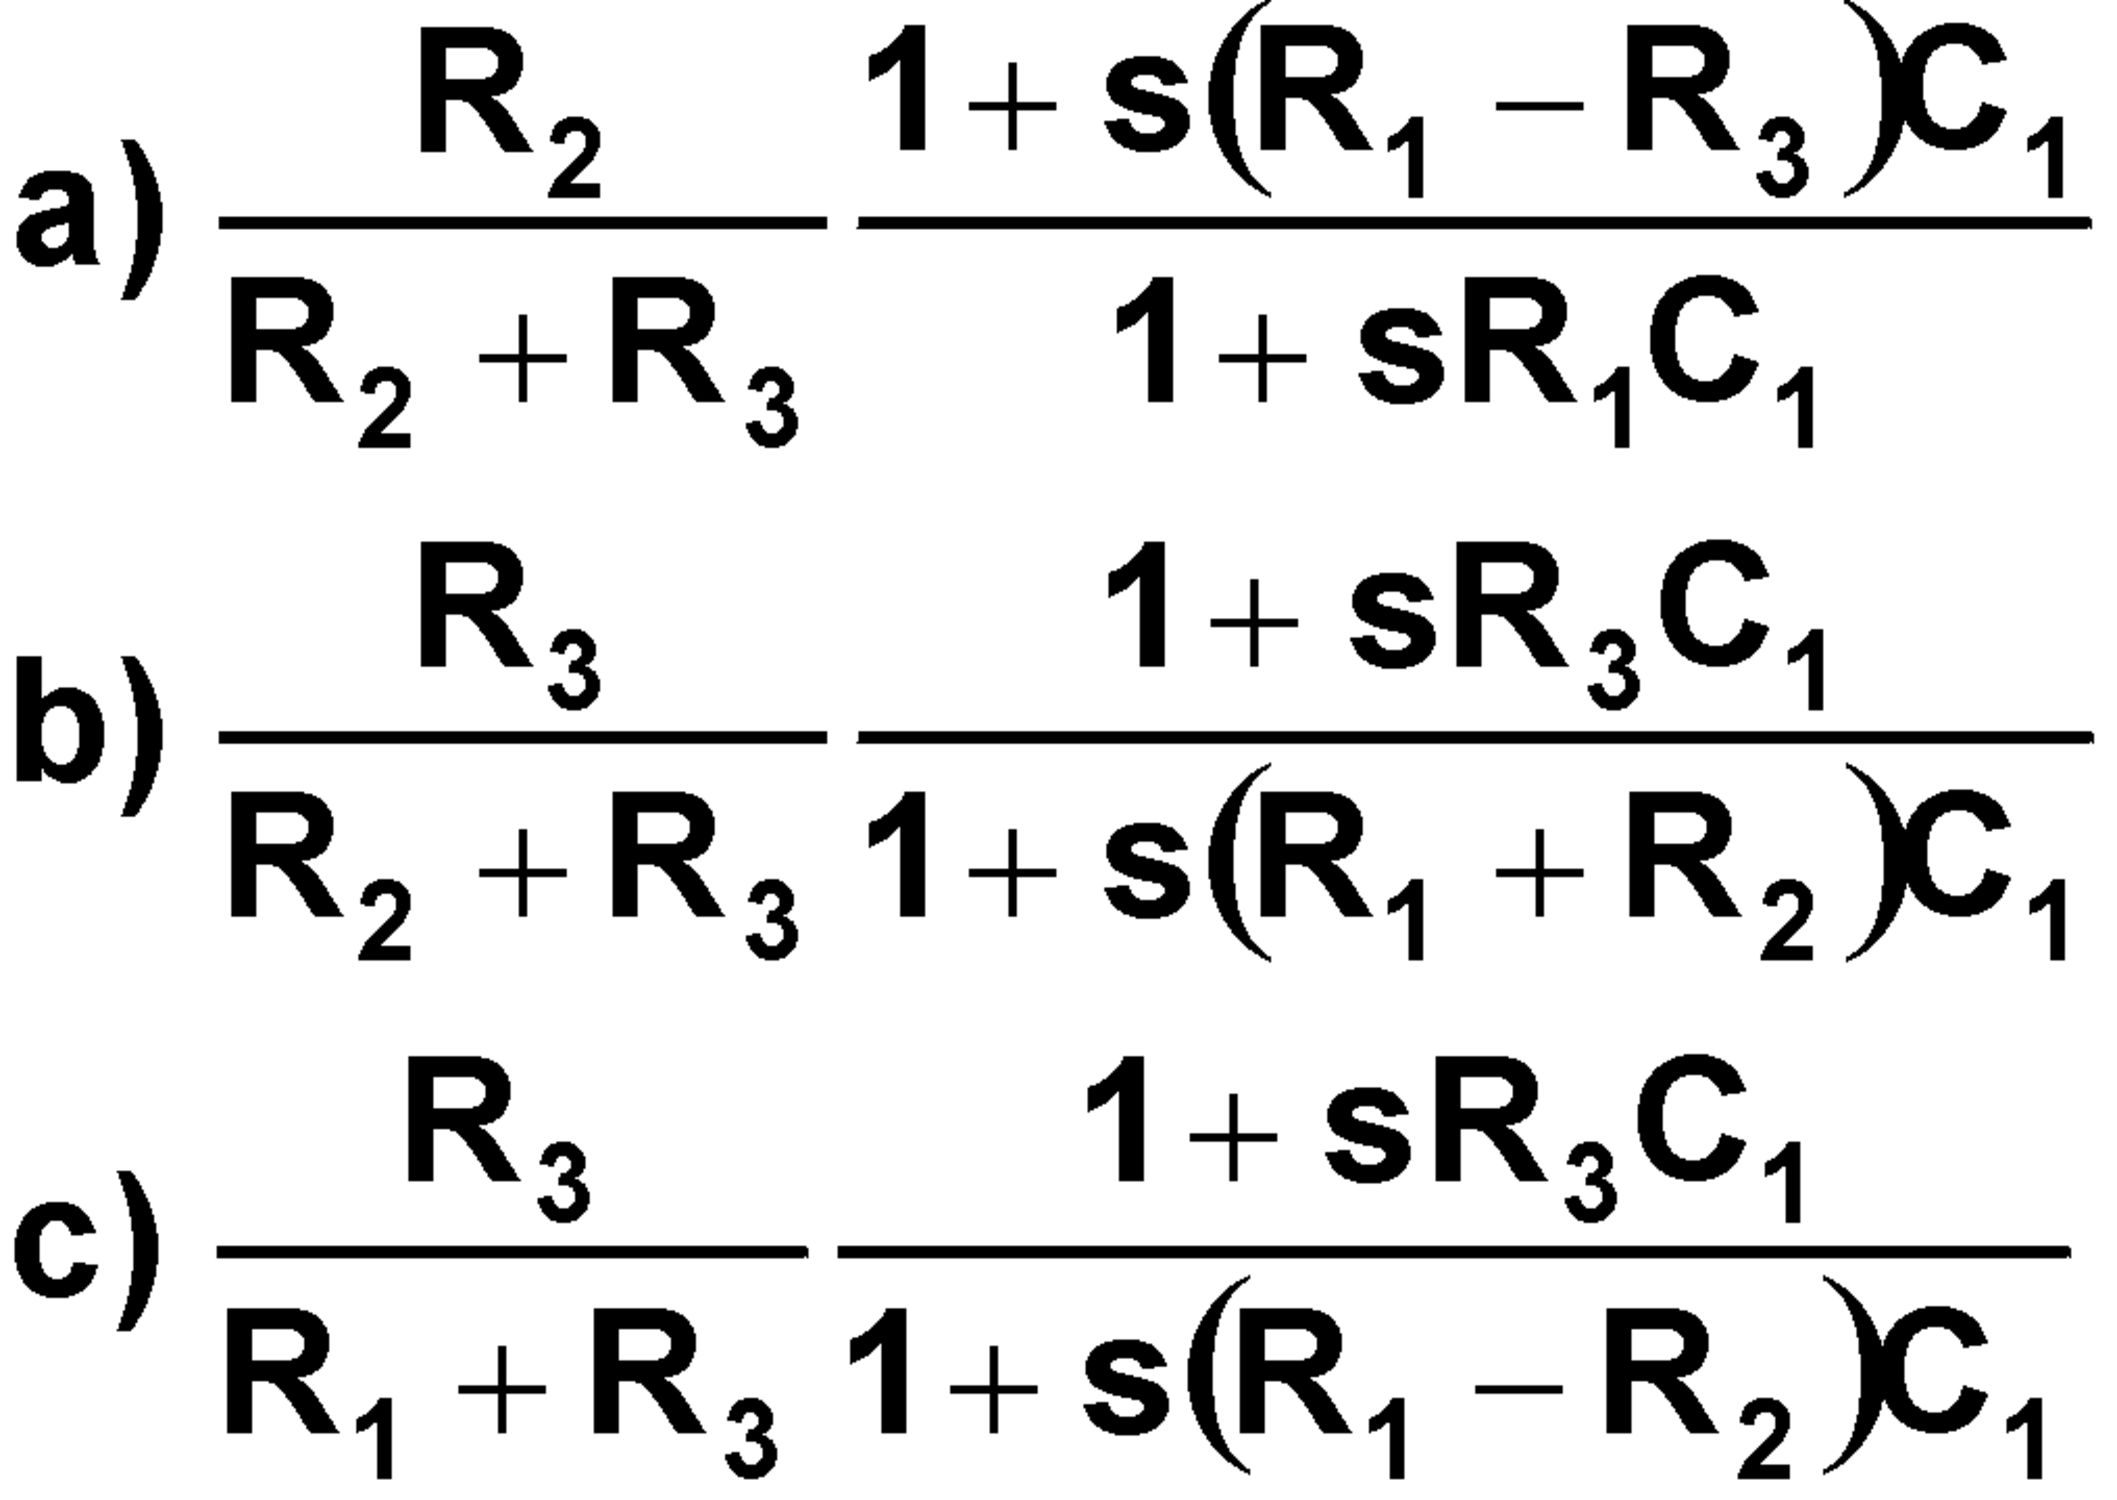
\includegraphics[width=.3\linewidth]{img/elettronicaEs/trasferimento.pdf}
\caption{Circuito con amplificatore invertente e possibili funzioni di trasferimento.}
\label{img:trasferimento}
\end{figure}


\subsection{Esercizio}

Difficoltà: ***\\

Dato il circuito di figura \ref{img:BJT1}, determinare il punto di lavoro $Q=(I_C, V_{CE})$ del BJT (si 
trascuri l'effetto Early).\\

Dati
\begin{itemize}
\item $R_B=270\,k\Omega$ 
\item $R_C=1,2\,k\Omega$ 
\item $V_{CC}=20\,V$ 
\item $V_{BE}=0,7\,V$
\item $\beta_F=150$
\end{itemize}

RISPOSTE: $I_C = 6,46\,mA$, $V_{CE} = 12,24\,V$

\begin{figure}[H]
\centering
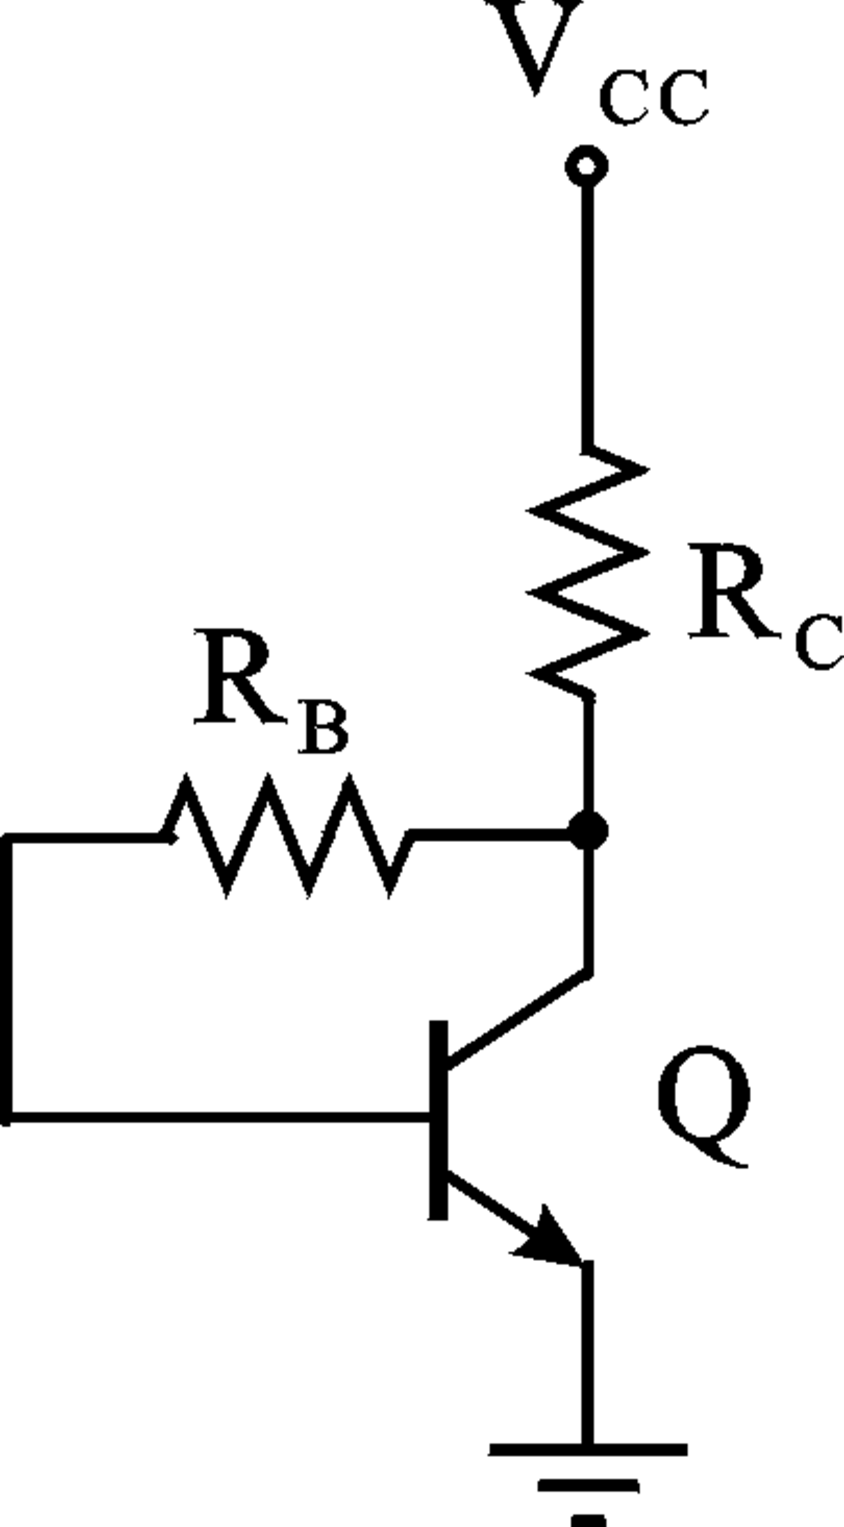
\includegraphics[width=.1\linewidth]{img/elettronicaEs/BJT1.pdf}
\caption{Circuito di polarizzazione con BJT.}
\label{img:BJT1}
\end{figure}


\subsection{Esercizio}

Difficoltà: **\\

Dato il circuito di figura \ref{img:MOSpiccolo1}, che rappresenta il modello dinamico equivalente di un 
amplificatore a transistore MOS polarizzato con una corrente di drain a riposo di $2\,mA$ (a $25^{\circ}C$), 
determinare il valore della resistenza di ingresso $R_{IN}$ indicata in figura (nel calcolo del $g_m$ si 
trascuri l'effetto di modulazione della lunghezza di canale).\\

Dati
\begin{itemize}
\item $R_1=100\,k\Omega$ 
\item $R_2=1\,k\Omega$
\item $R_3=100\,k\Omega$ 
\item $V_T=3\,V$ 
\item $I_{DSS}=V_T 2\mu C_{ox} {W \over 2L}=8\,mA$
\end{itemize}

RISPOSTA: $R_{IN} = 375,8\,\Omega$


\subsection{Esercizio}

Difficoltà: **\\

Dato il circuito di figura \ref{img:MOSpiccolo1}, che rappresenta il modello dinamico equivalente di un 
amplificatore a transistore MOS polarizzato con una corrente di drain a riposo di $2\,mA$ (a $25^{\circ}C$), 
determinare il valore della resistenza di ingresso $R_{IN}$ indicata in figura (nel calcolo del $g_m$ si 
trascuri l'effetto di modulazione della lunghezza di canale).\\

Dati
\begin{itemize}
\item $R_1=30\,k\Omega$ 
\item $R_2=165\,k\Omega$
\item $R_3=5\,k\Omega$ 
\item $V_T=2,5\,V$ 
\item $I_{DSS}=V_T 2\mu C_{ox} {W \over 2L}=8\,mA$
\end{itemize}

\begin{figure}[H]
\centering
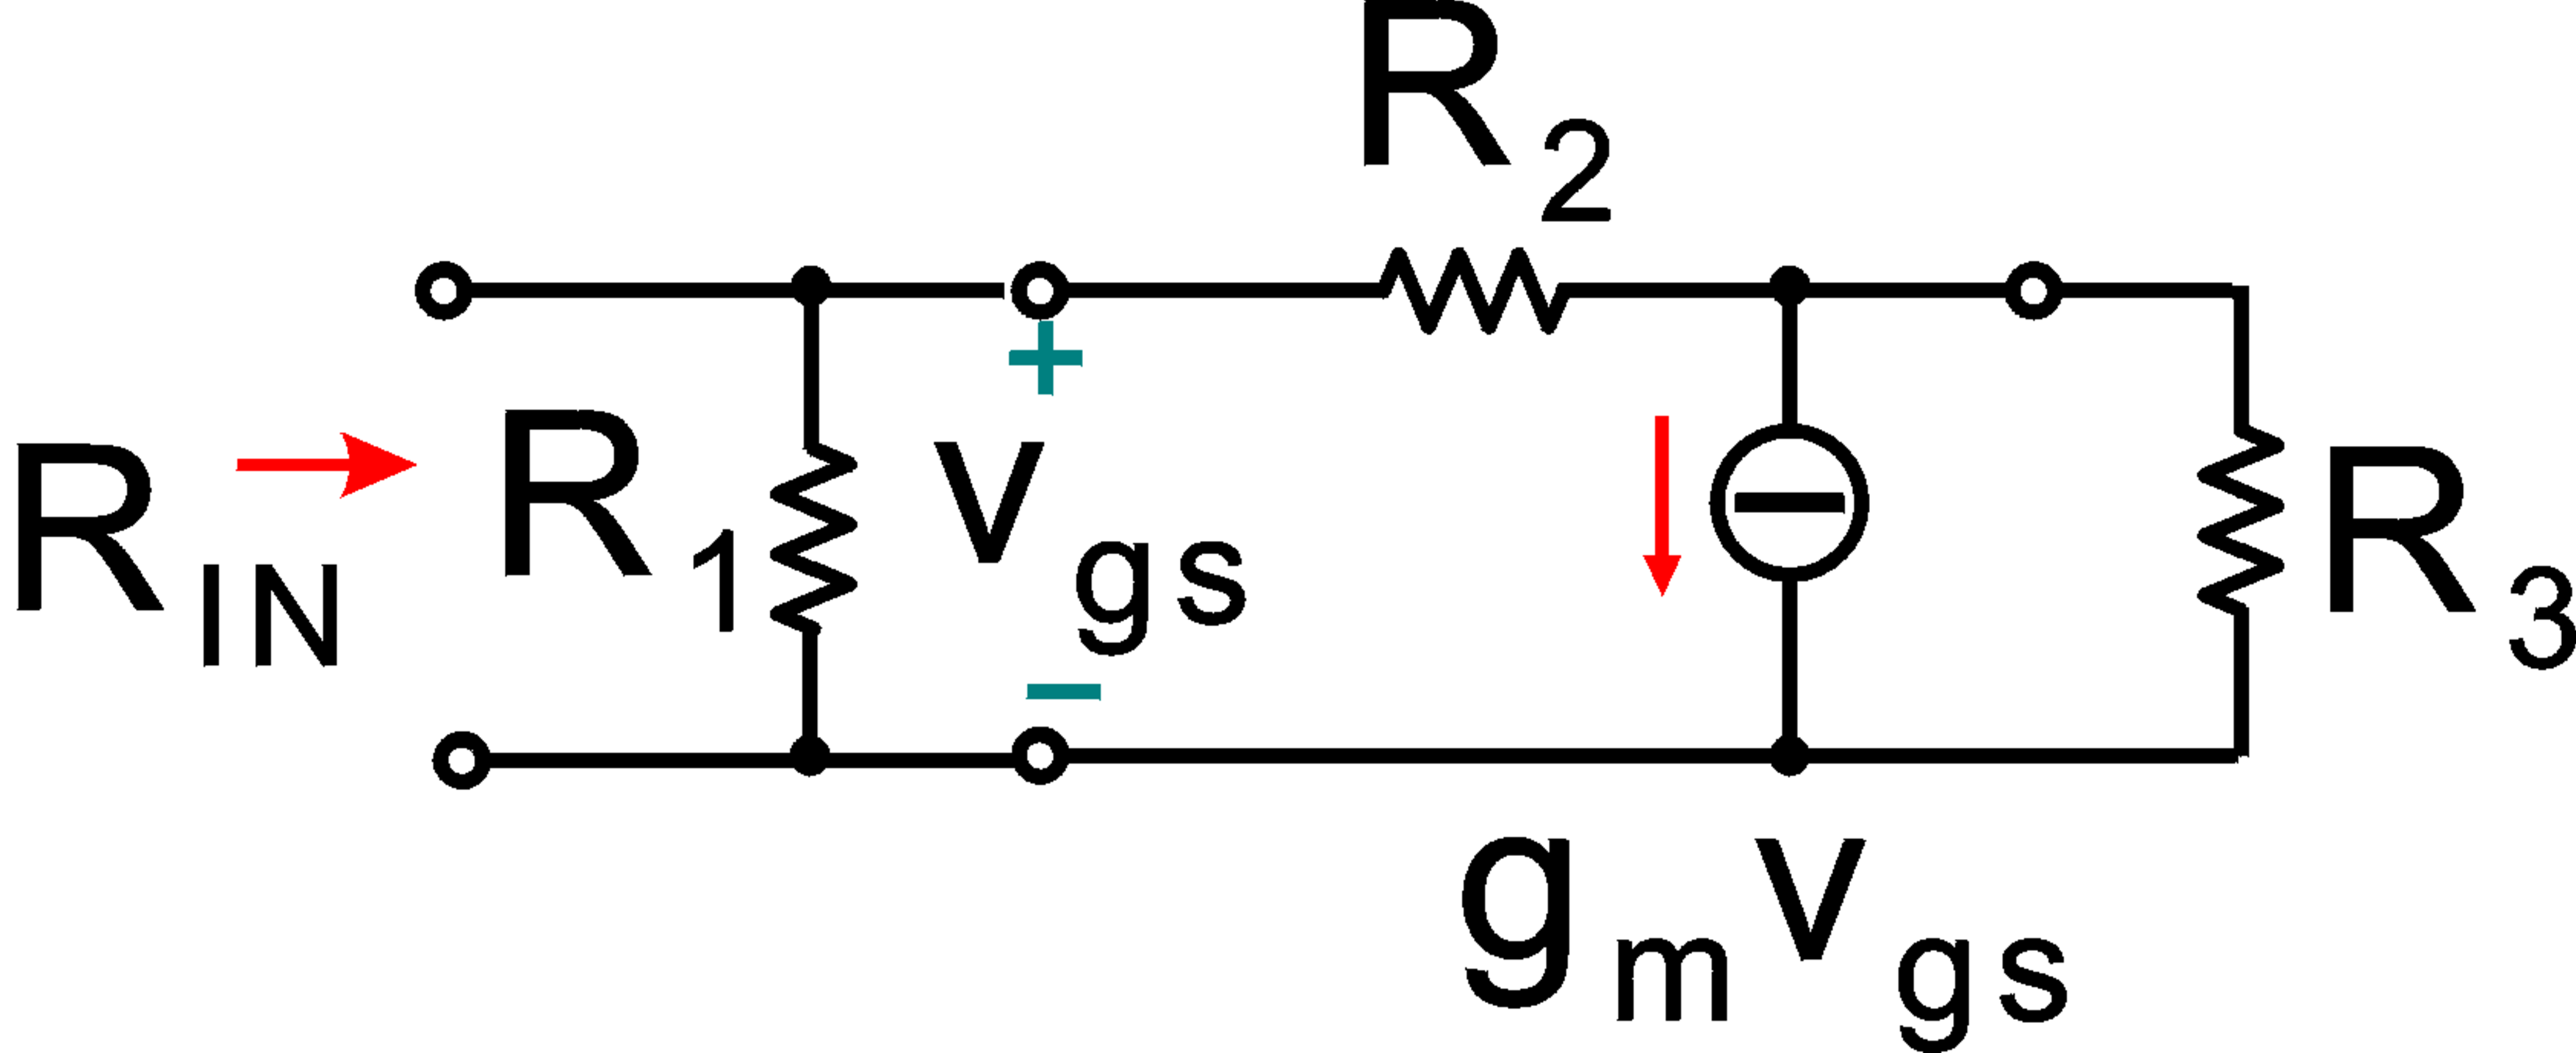
\includegraphics[width=.5\linewidth]{img/elettronicaEs/MOSpiccolo1.pdf}
\caption{Modello equivalente dinamico per MOSFET.}
\label{img:MOSpiccolo1}
\end{figure}

\subsection{Esercizio}

Difficoltà: **\\

Dato il circuito di figura \ref{img:MOSpiccolo2}, che rappresenta il modello dinamico equivalente di un 
amplificatore a transistore MOS polarizzato con una corrente di drain a riposo di $0,4\,mA$ (a $25^{\circ}C$),
determinare il valore della resistenza equivalente $R_{eq}$ indicata in figura (nel calcolo del $g_m$ si 
trascuri l'effetto di modulazione della lunghezza di canale).\\

Dati
\begin{itemize}
\item $R_1=50\,k\Omega$
\item $r_o=10\,k\Omega$
\item $V_T=6\,V$ 
\item $I_{DSS}=V_T2\mu C_{ox}{W\over 2L}=6\,mA$
\end{itemize}

\begin{figure}[H]
\centering
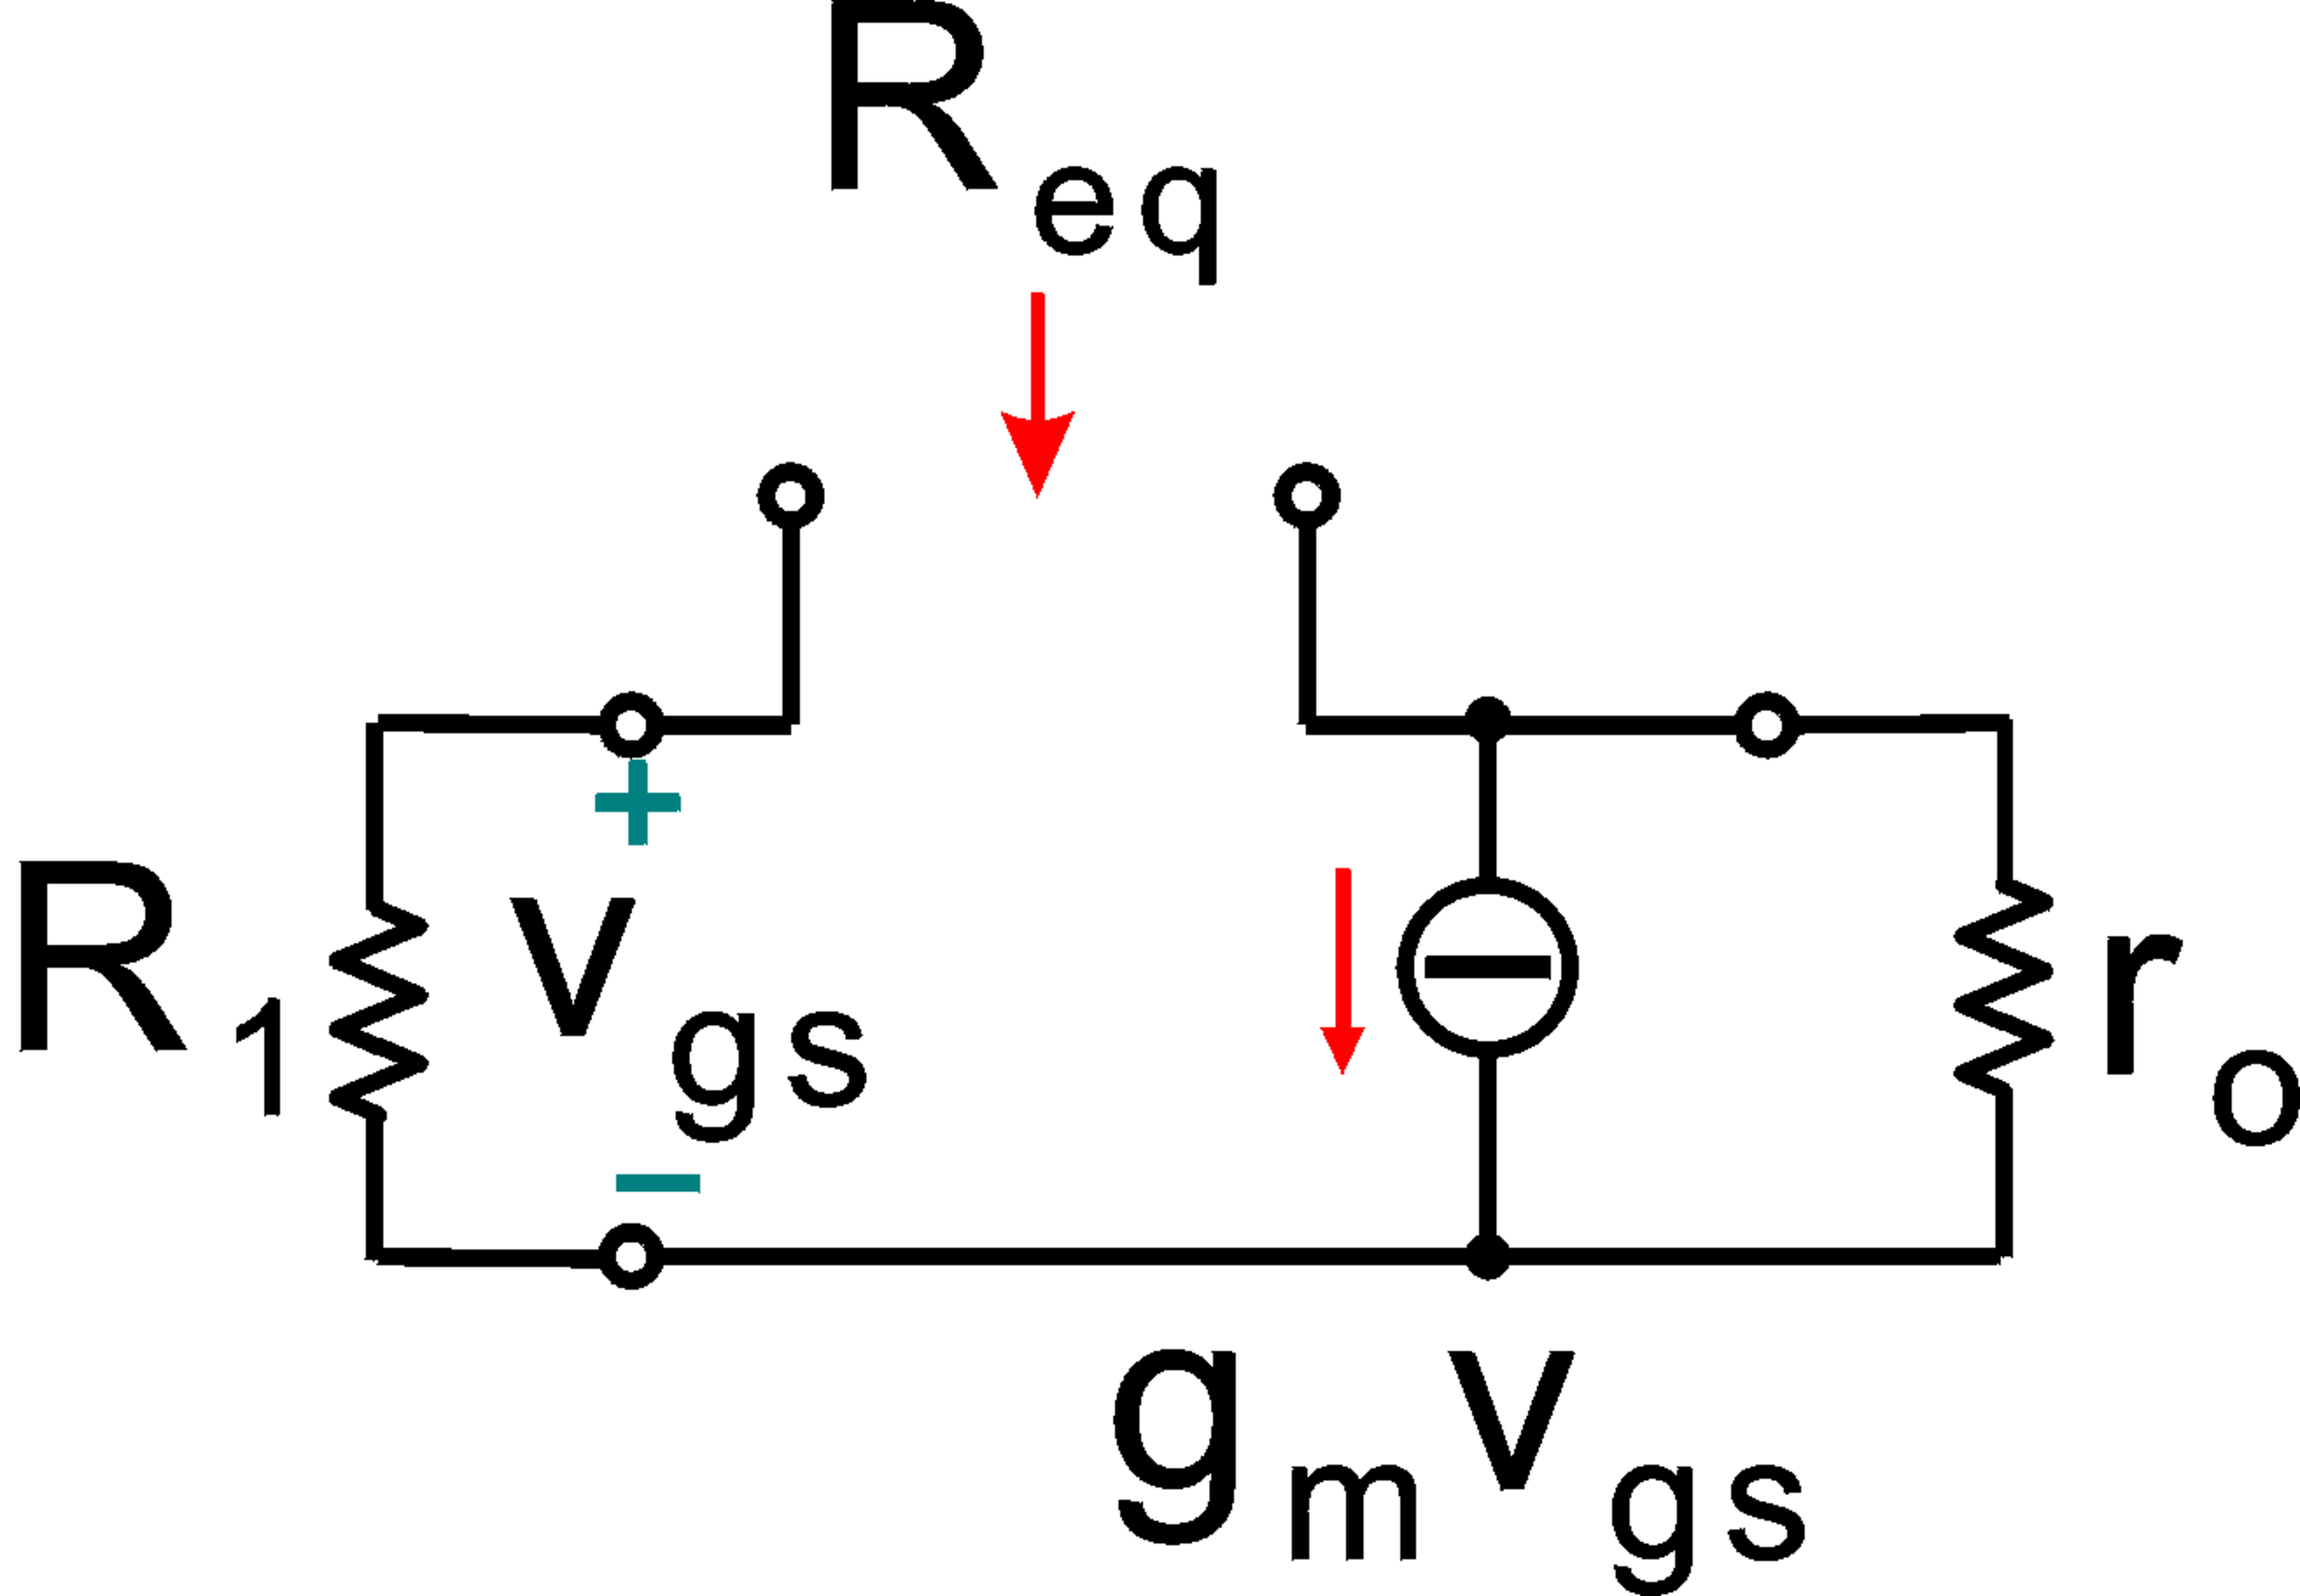
\includegraphics[width=.5\linewidth]{img/elettronicaEs/MOSpiccolo2.pdf}
\caption{Modello equivalente dinamico per MOSFET.}
\label{img:MOSpiccolo2}
\end{figure}


\subsection{Esercizio}

Difficoltà: ***\\

Dato il circuito di figura \ref{img:MOSampli}, che impiega un amplificatore operazionale ideale, sapendo 
che la corrente di drain $I_D$ a riposo del transistore $Q_1$ vale $0,8\,mA$ e che la tensione di uscita 
$V_o$ in continua vale $2\,V$, determinare il valore della tensione $V_R$ al morsetto non invertente 
dell'amplificatore operazionale ed il valore del generatore di corrente $I_A$.\\

Dati
\begin{itemize}
\item $R_G=220\,k\Omega$
\item $R_1=10\,k\Omega$
\item $R_S=5.6\,k\Omega$
\item $R_F=10\,k\Omega$
\item $V_{DD}=V_{SS}=18\,V$
\item $Q_1$ MOSFET n-channel ad arricchimento
\item $V_{TH}=2,5\,V$
\item $I_{DSS}={1\over 2L}\mu C_{ox}V_{TH}2W=6\,mA$
\end{itemize}

\begin{figure}[H]
\centering
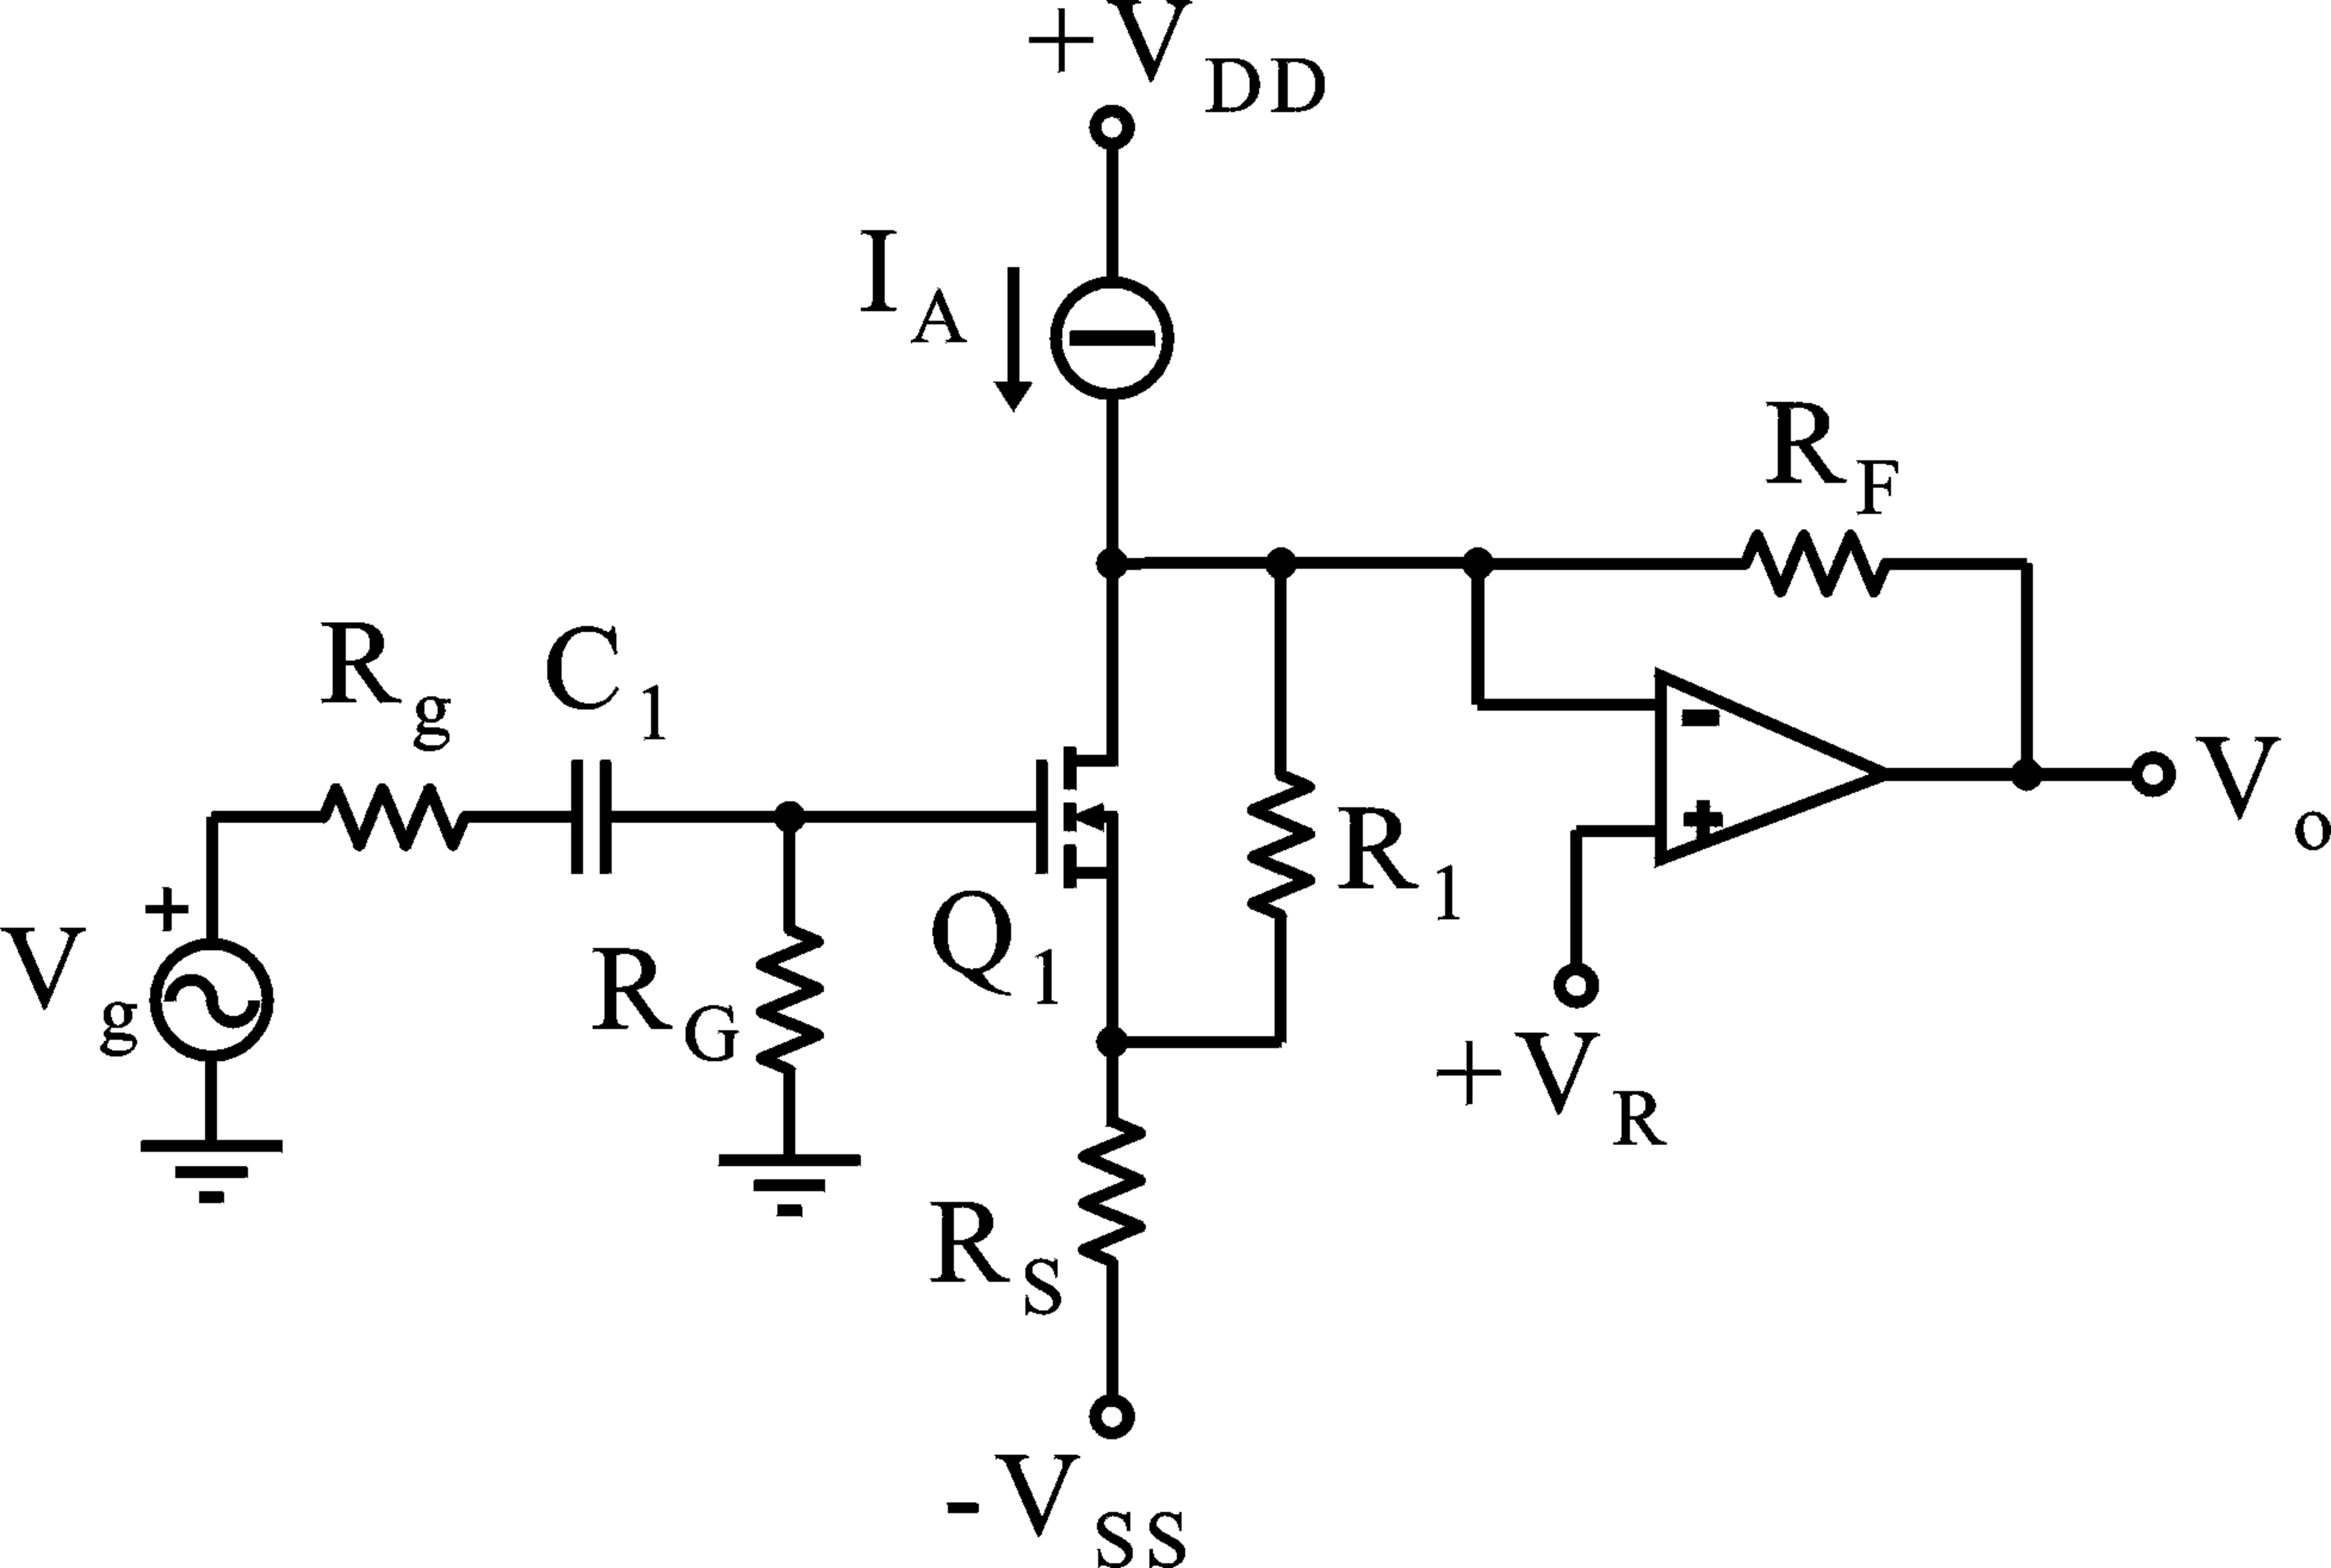
\includegraphics[width=.5\linewidth]{img/elettronicaEs/MOSampli.pdf}
\caption{MOSFET con amplificatore operazionale.}
\label{img:MOSampli}
\end{figure}


\subsection{Esercizio}

Difficoltà: ***\\

Il circuito di figura \ref{img:transdiodo2}, che utilizza un diodo considerato ideale, presenta una 
transcaratteristica $V_o = f(V_i)$ composta da due segmenti, ciascuno di equazione $V_o=m V_i+q$, con un 
punto di spezzamento in corrispondenza del valore della tensione d'ingresso $V_{iTH}$.\\ 

Determinare:
\begin{enumerate}
\item il valore della tensione di spezzamento $V_{iTH}$;
\item la pendenza $m_1$ del segmento della transcaratteristica per $V_i < V_{iTH}$;
\item il termine noto $q_1$ del segmento della transcaratteristica per $V_i < V_{iTH}$;
\item la pendenza $m_2$ del segmento della transcaratteristica per $V_i > V_{iTH}$;
\item il termine noto $q_2$ del segmento della transcaratteristica per $V_i > V_{iTH}$.
\end{enumerate}

Dati
\begin{itemize}
\item $R_1=1\,k\Omega$ 
\item $R_2=3\,k\Omega$
\item $R_3=6\,k\Omega$
\item $I_A=2\,mA$
\end{itemize}

RISPOSTE: $V_{iTH} = 8\,V$, $m_1 = $, $q_1 = 0\,V$, $m_2 = $, $q_2 = $

\begin{figure}[H]
\centering
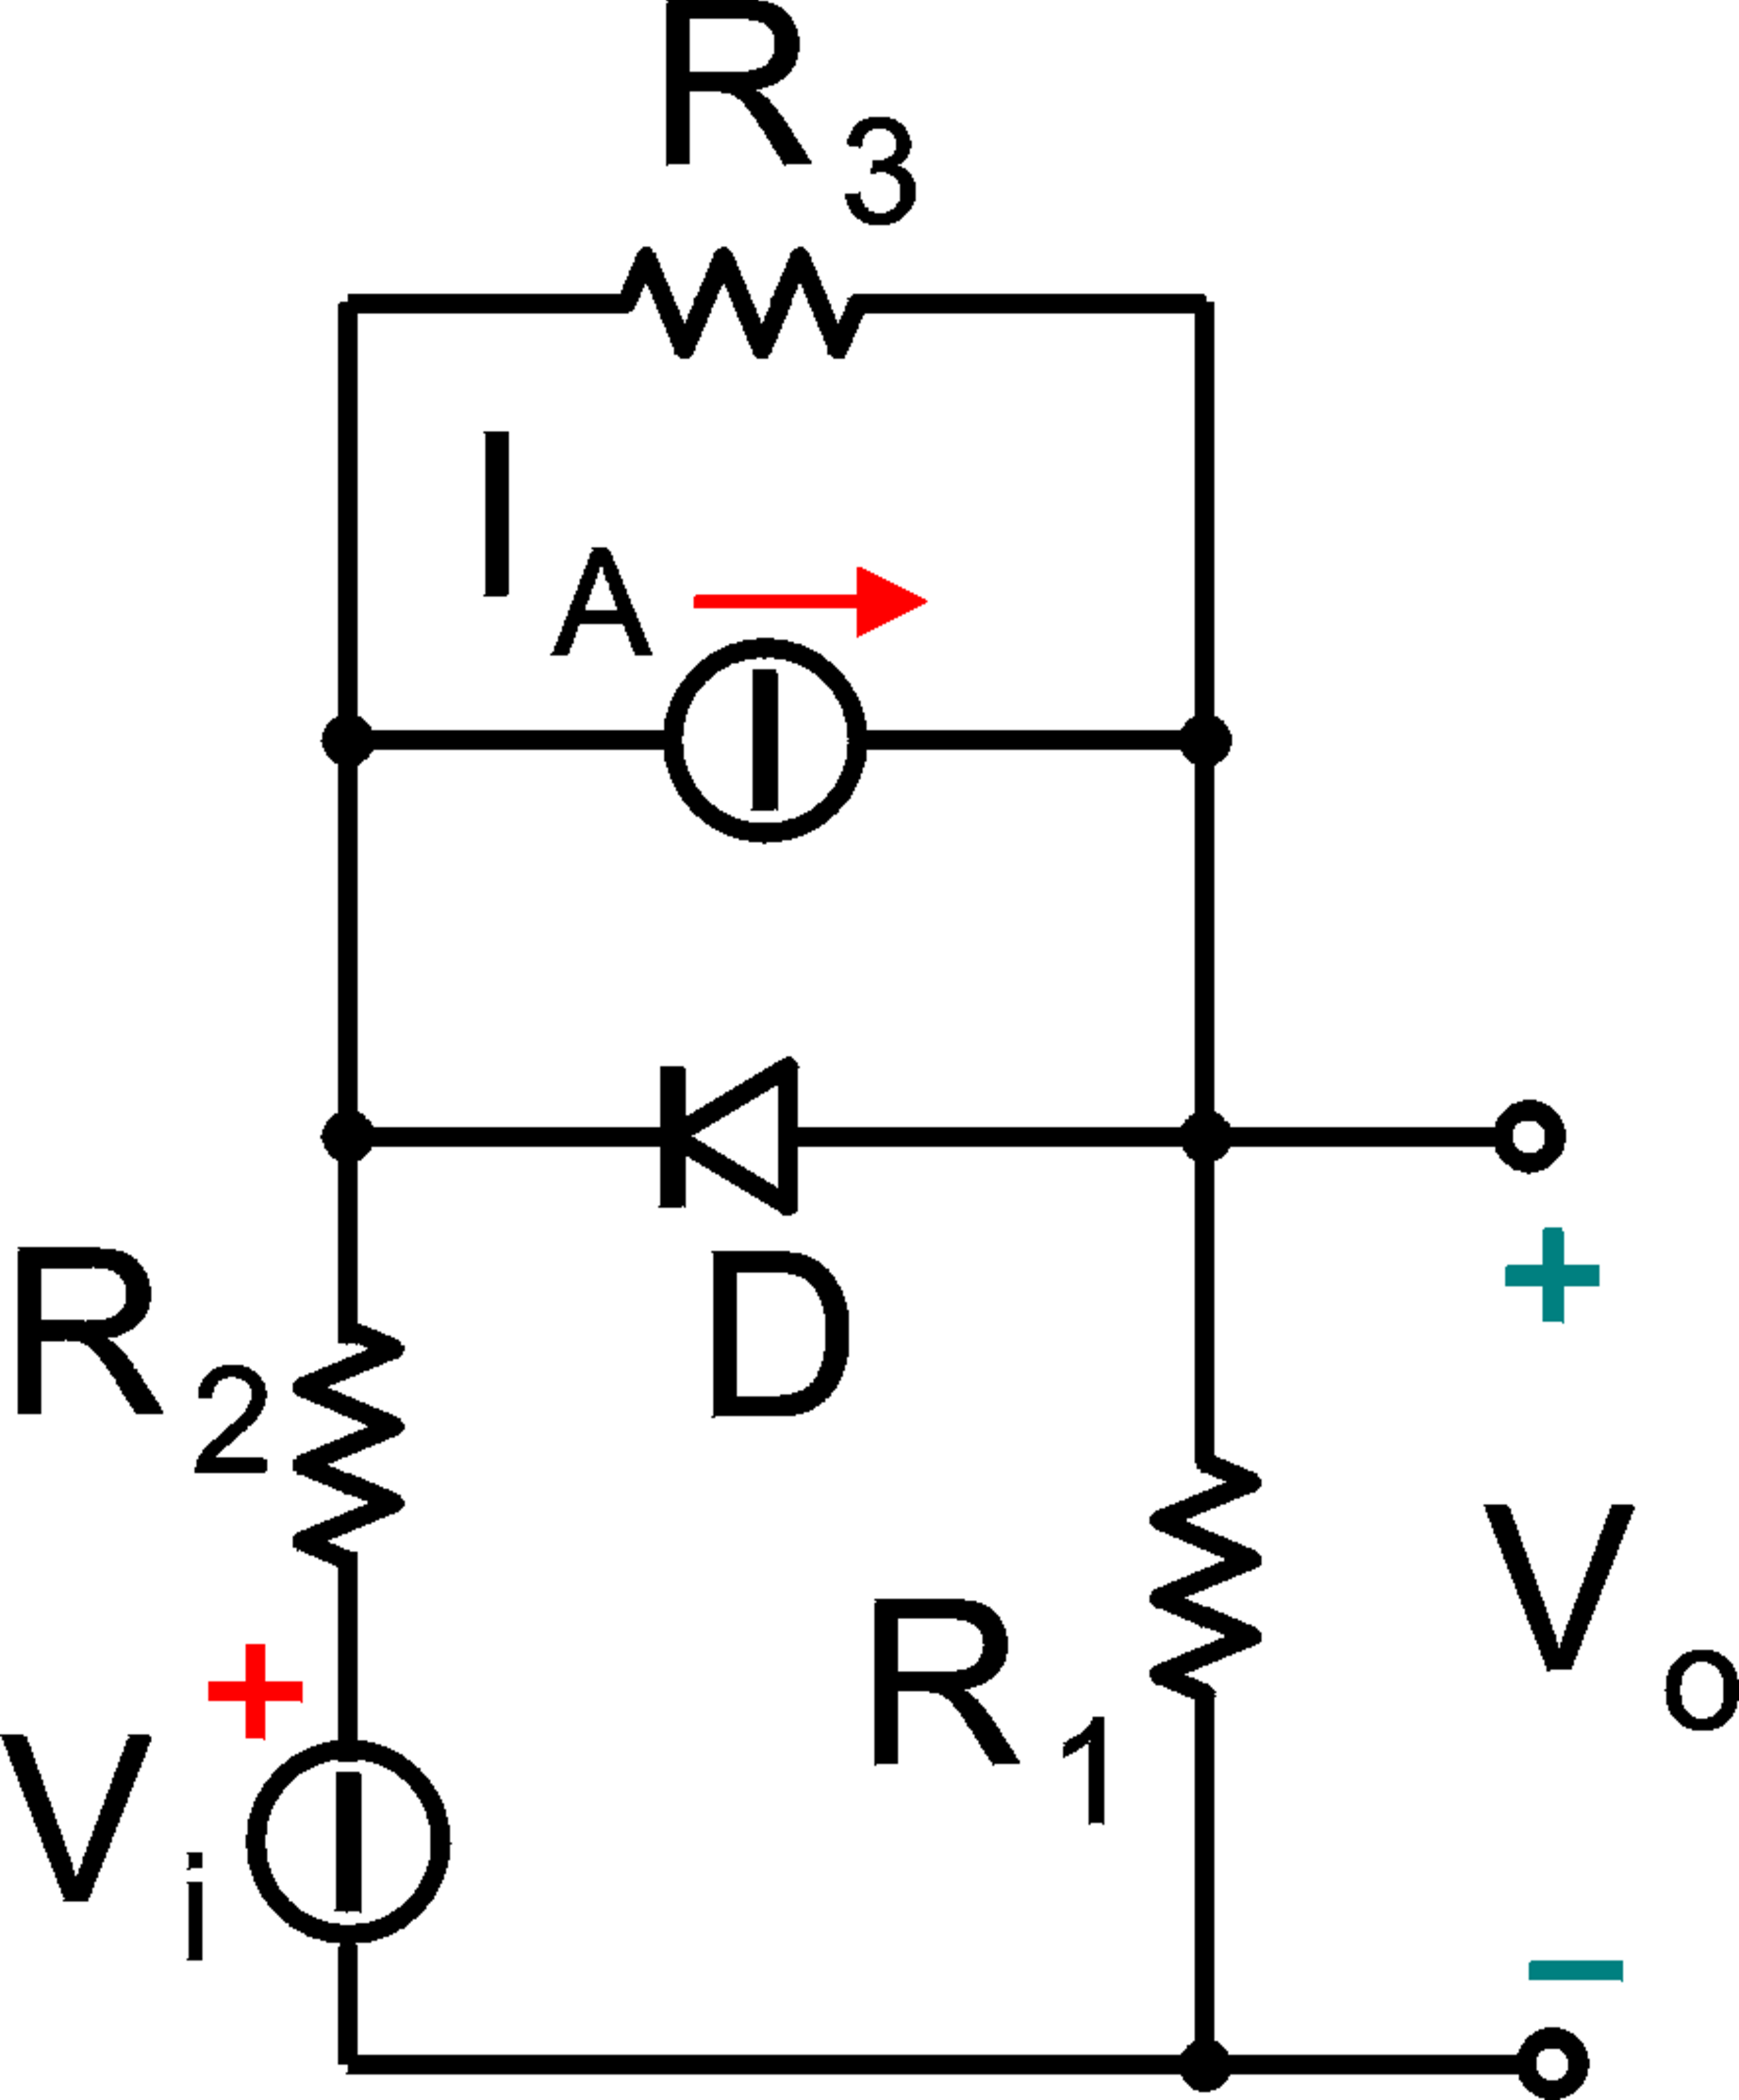
\includegraphics[width=.3\linewidth]{img/elettronicaEs/transdiodo2.pdf}
\caption{Trovare la transcaratteristica del circuito.}
\label{img:transdiodo2}
\end{figure}


\subsection{Esercizio}
 
Difficoltà: ***\\
 
Il circuito di figura \ref{img:transdiodo3}, che utilizza un diodo considerato ideale, presenta una
transcaratteristica $V_o = f(V_i)$ composta da due segmenti, ciascuno di equazione $V_o=m V_i+q$, con un
punto di spezzamento in corrispondenza del valore della tensione d'ingresso $V_{iTH}$.\\

Determinare:
\begin{enumerate}
\item il valore della tensione di spezzamento $V_{iTH}$;
\item la pendenza $m_1$ del segmento della transcaratteristica per $V_i < V_{iTH}$;
\item il termine noto $q_1$ del segmento della transcaratteristica per $V_i < V_{iTH}$;
\item la pendenza $m_2$ del segmento della transcaratteristica per $V_i > V_{iTH}$;
\item il termine noto $q_2$ del segmento della transcaratteristica per $V_i > V_{iTH}$.
\end{enumerate}

Dati
\begin{itemize}
\item $R_1=1\,k\Omega$ 
\item $R_2=3\,k\Omega$ 
\item $R_3=2\,k\Omega$ 
\item $I_A=2\,mA$
\end{itemize}

RISPOSTE: $V_{iTH} = \,V$, $m_1 = 0,33$, $q_1 = \,V$, $m_2 = 0$, $q_2 = \,V$

\begin{figure}[H]
\centering
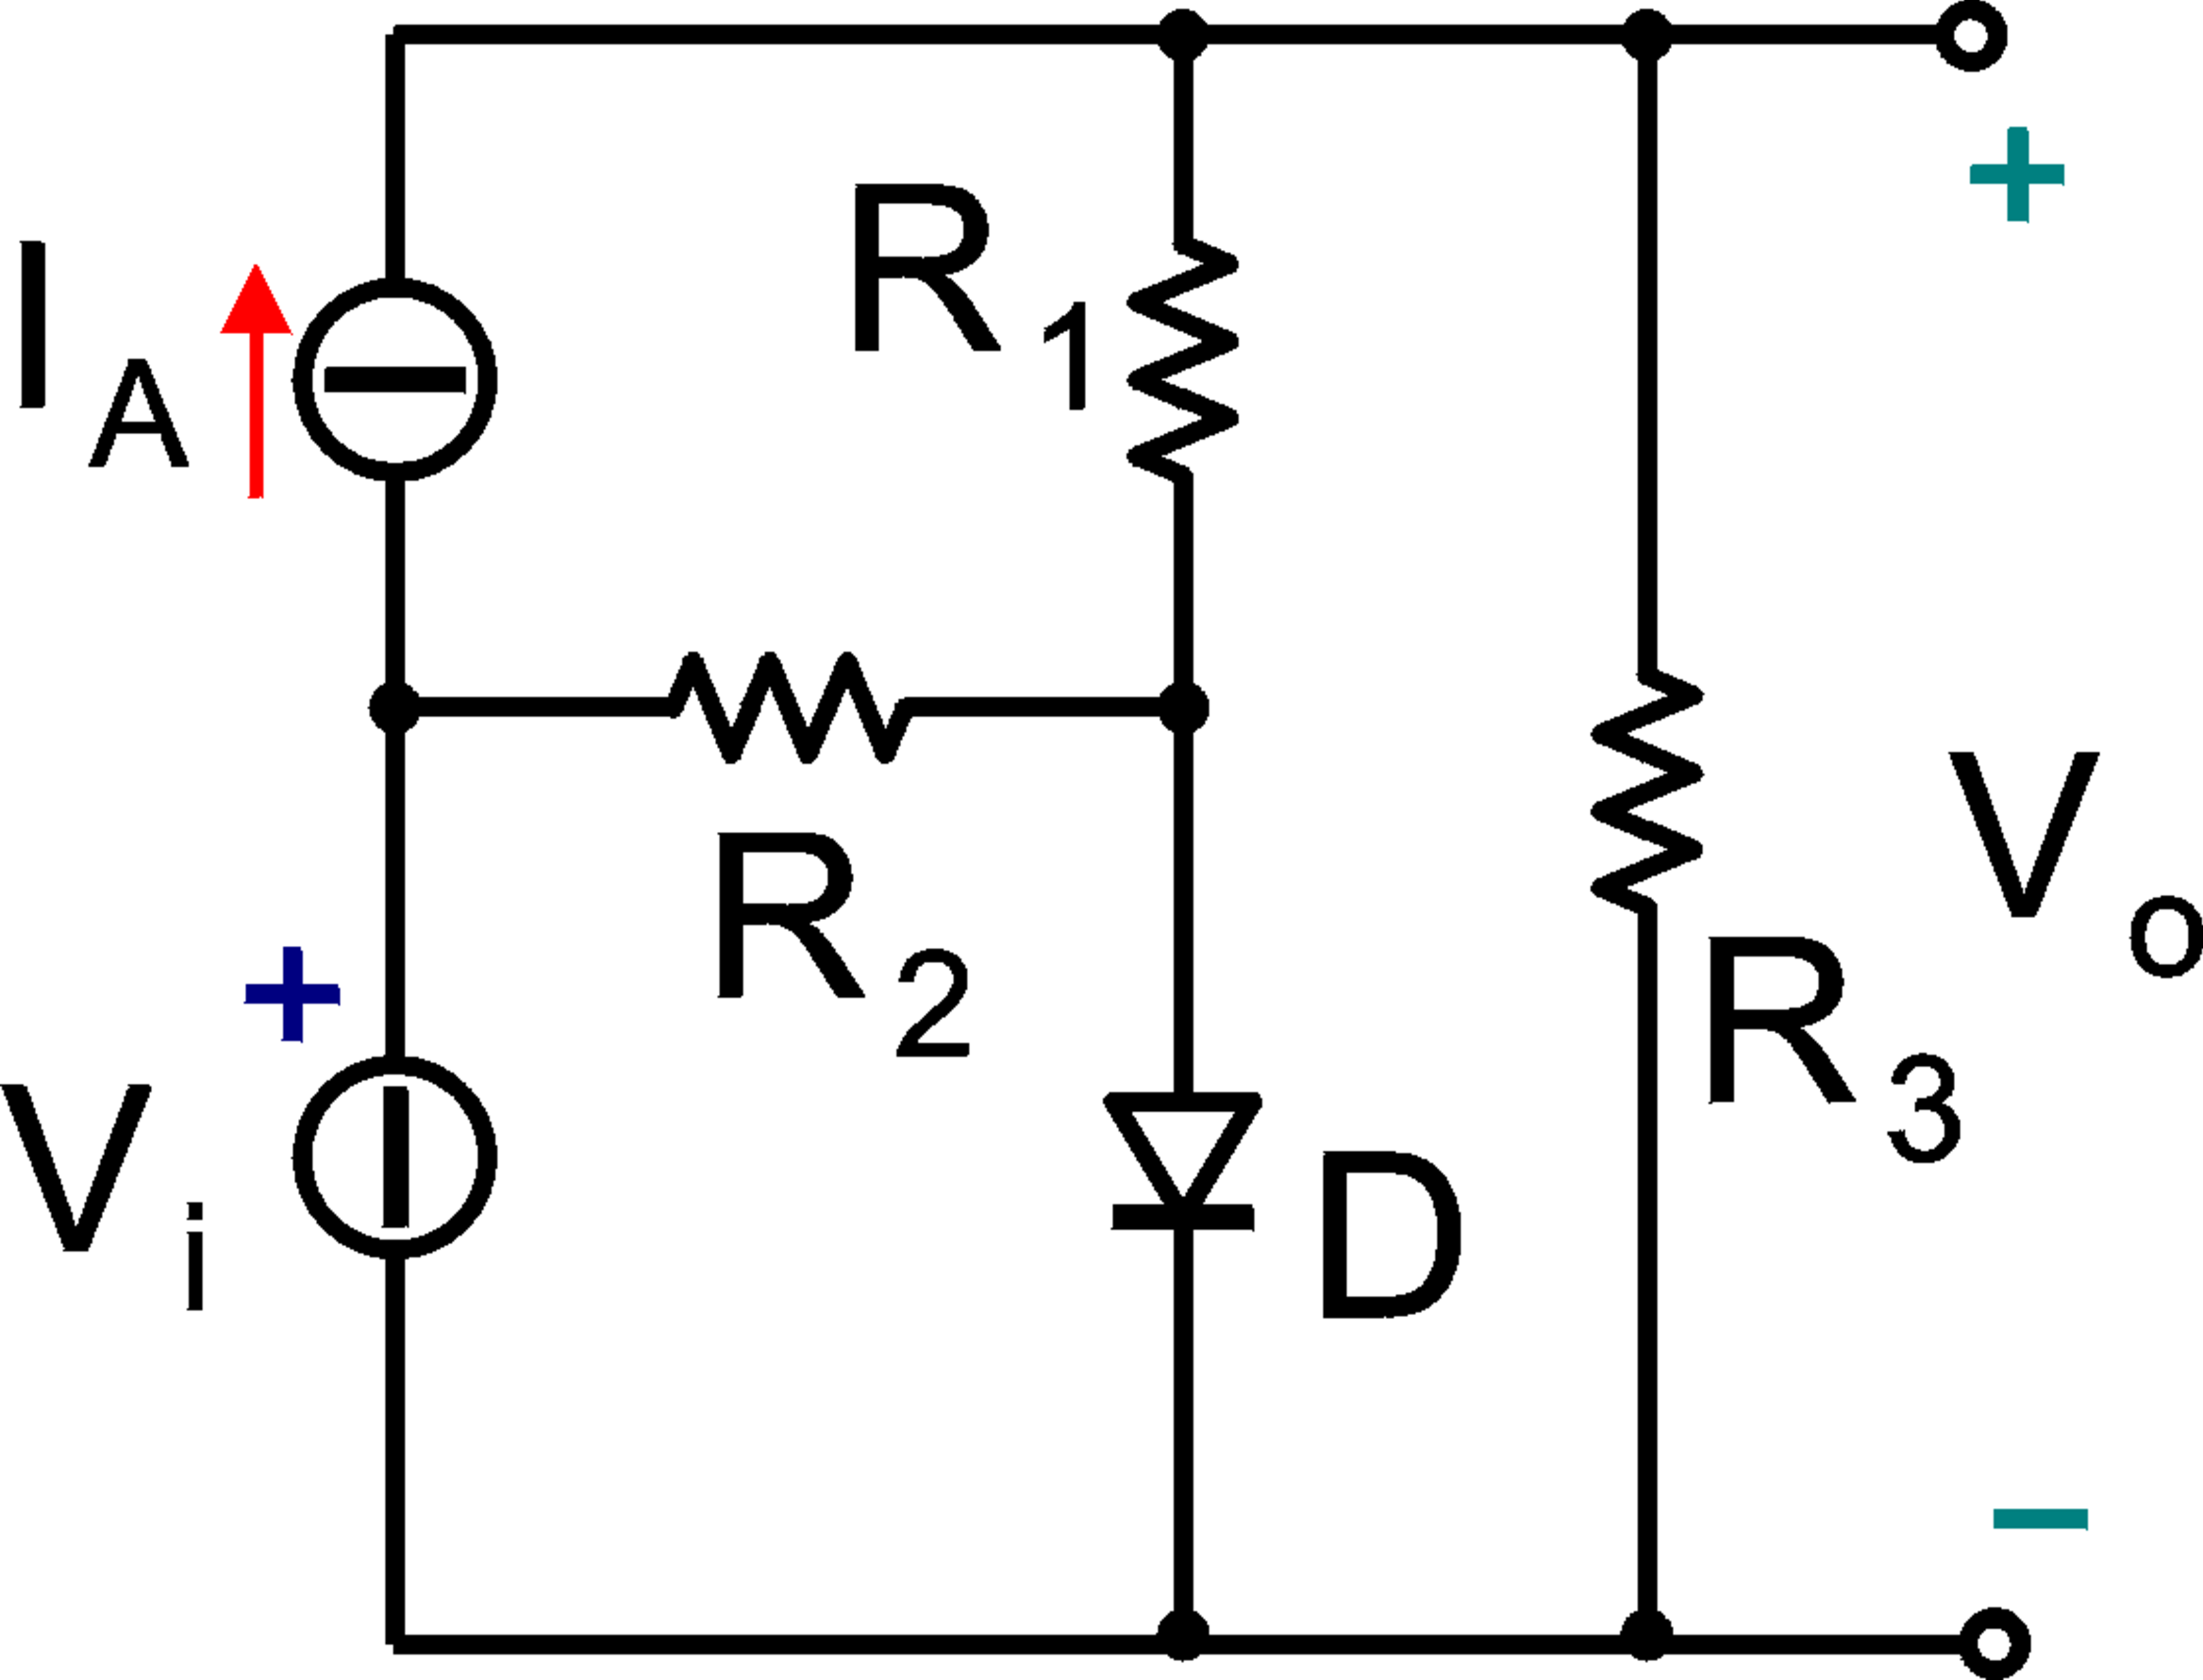
\includegraphics[width=.3\linewidth]{img/elettronicaEs/transdiodo3.pdf}
\caption{Trovare la transcaratteristica del circuito.}
\label{img:transdiodo3}
\end{figure}


\subsection{Esercizio}

Difficoltà: **\\

Nell'amplificatore di figura \ref{img:invertente4R}, $R_1 = R_2 = R_4 = 100\,k\Omega$. Qual'è il valore di 
$R_3$ da utilizzare per ottenere un guadagno il più vicino possibile a $-120$?\\

RISPOSTA: $R_3 = 847 \Omega$

\begin{figure}[H]
\centering
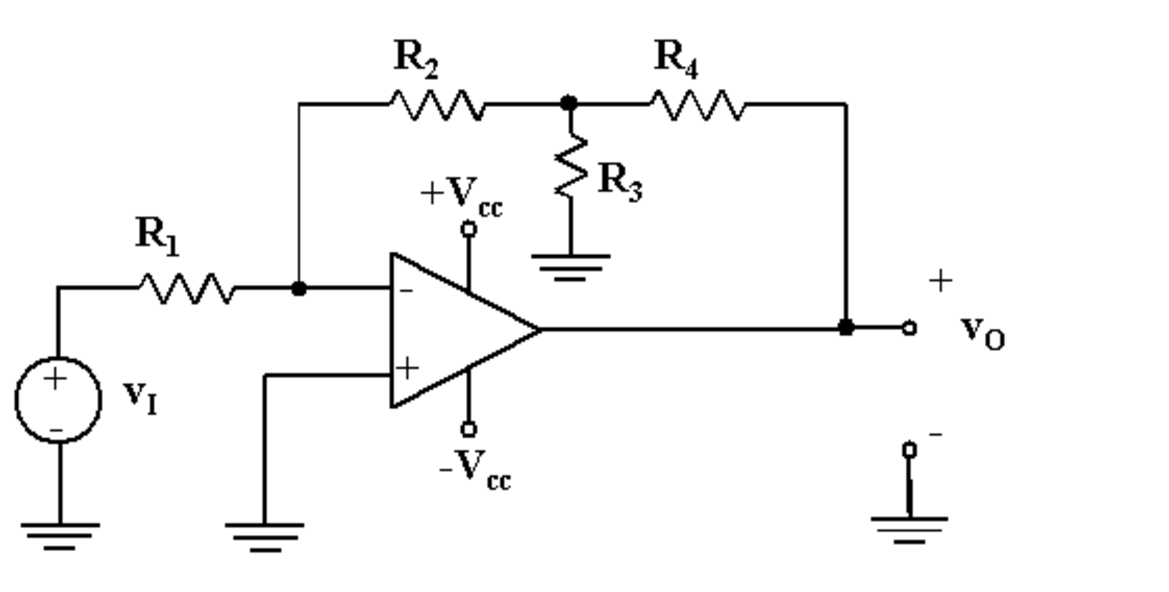
\includegraphics[width=.4\linewidth]{img/elettronicaEs/invertente4R.pdf}
\caption{Amplificatore in configurazione invertente con 4 resistenze.}
\label{img:invertente4R}
\end{figure}

\end{document}
